%===================================== CHAP 5 =================================

\chapter{Results and discussion}
Gi et overblikk over kapitellet her.

The entire simulation process, including set-up of model and calculations, were performed on a desktop computer equipped with 32 GB RAM and an Intel Core i7-3930K CPU with 6 physical cores (each with 2 logical cores) operating at clockspeed 3.20 GHz, and running on a 64-bit Windows 7 operating system.
%%%%%%%%%%%%%%% NEW SECTION %%%%%%%%%%%%%%%
\section{Implementation of samples into COMSOL}
All samples presented in chapter \ref{chapter3} were implemented as a single cell with periodic conditions simulating the infinite periodic structure. The protruding gold semispheres lies in a square or rectangular lattice, while the densely packed distribution of the tilted GaSb cones were modeled as a hexagonal grating.

The model set-up is similar for all the structures, especially the gold hemispheroidal nanostructures, as they all have rectangular lattices and differ only by the numerical values of their sample parameters. The GaSb cones, being arranged in a hexagonal lattice, required certain adjustments which are discussed in section \ref{sec:implementation_gasb_cones} \text{\color{red}really?}. 

\subsection{Geometry and materials}
Creating the geometries in COMSOL is a straightforward manner of combining solid blocks and ellipsoids with Boolean operations as previously mentioned in. The mound region was created by first defining its cross-section, then sweeping it along the rim of the base of the Au particle, as depicted in figure \ref{fig:implementation_geometry_mound}. The finished geometries for all the samples can be seen in figure \ref{fig:implementation_geometry_samples}, while figure \ref{fig:implementation_ewfd_setup} shows the entire computational domain.
\begin{figure}[htb!]
    \begin{subfigure}{0.3\textwidth}
        \centering
        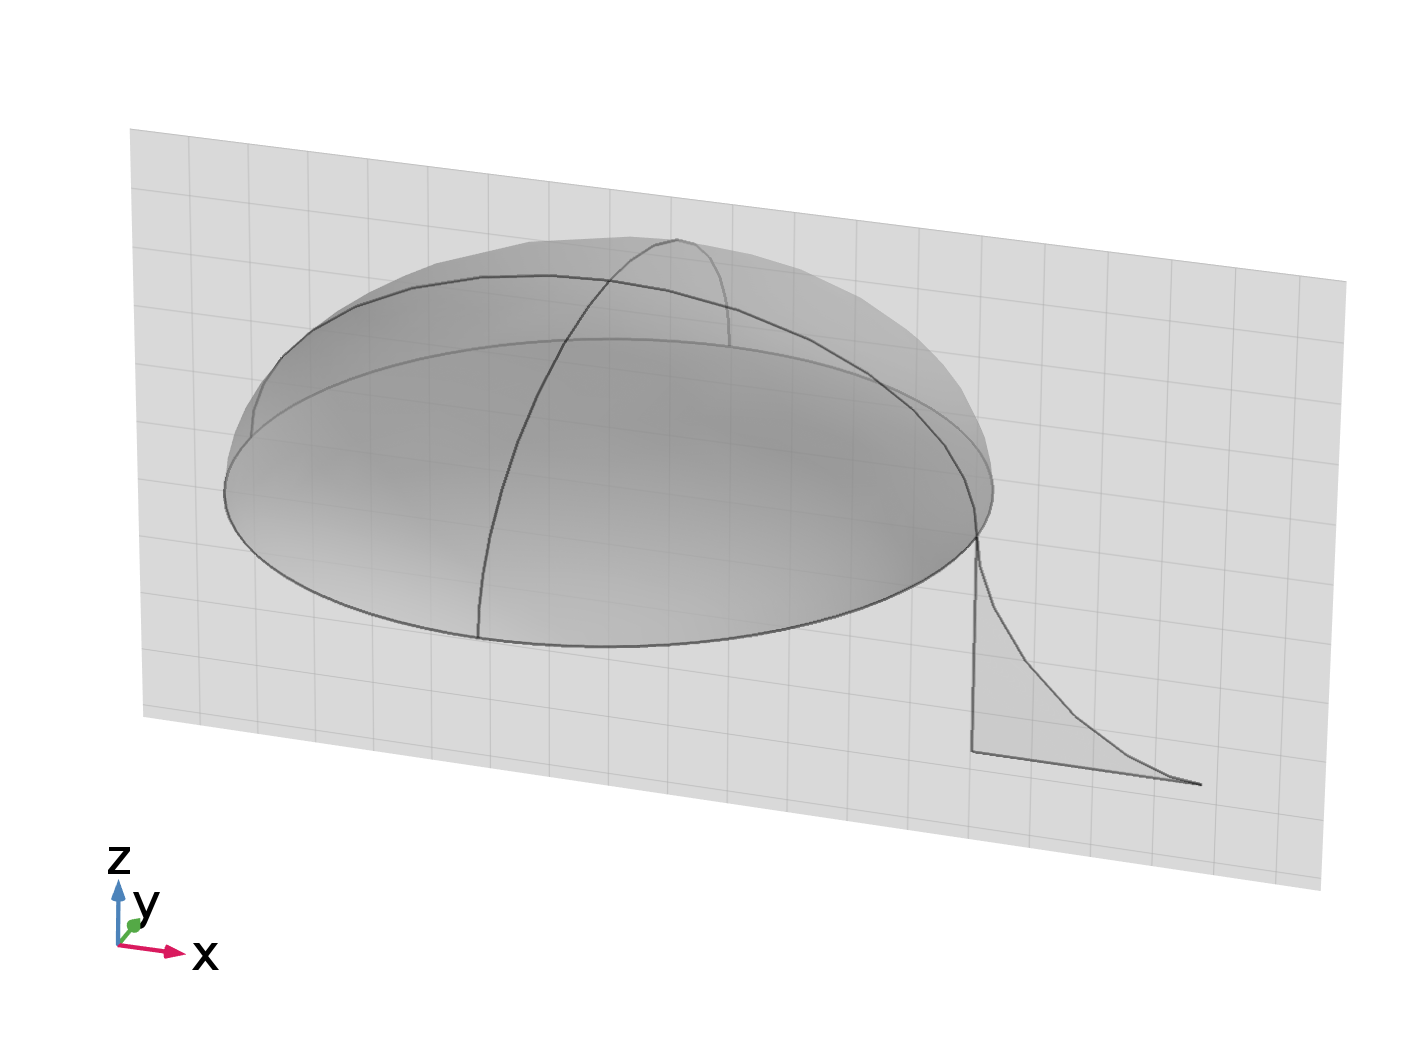
\includegraphics[width=0.8\linewidth, trim=0cm 0 0 0cm, clip]{figures/ch4/implem/geometry/Sample5A_mound_workplane.png}
    \end{subfigure}
    \begin{subfigure}{0.3\textwidth}
        \centering
        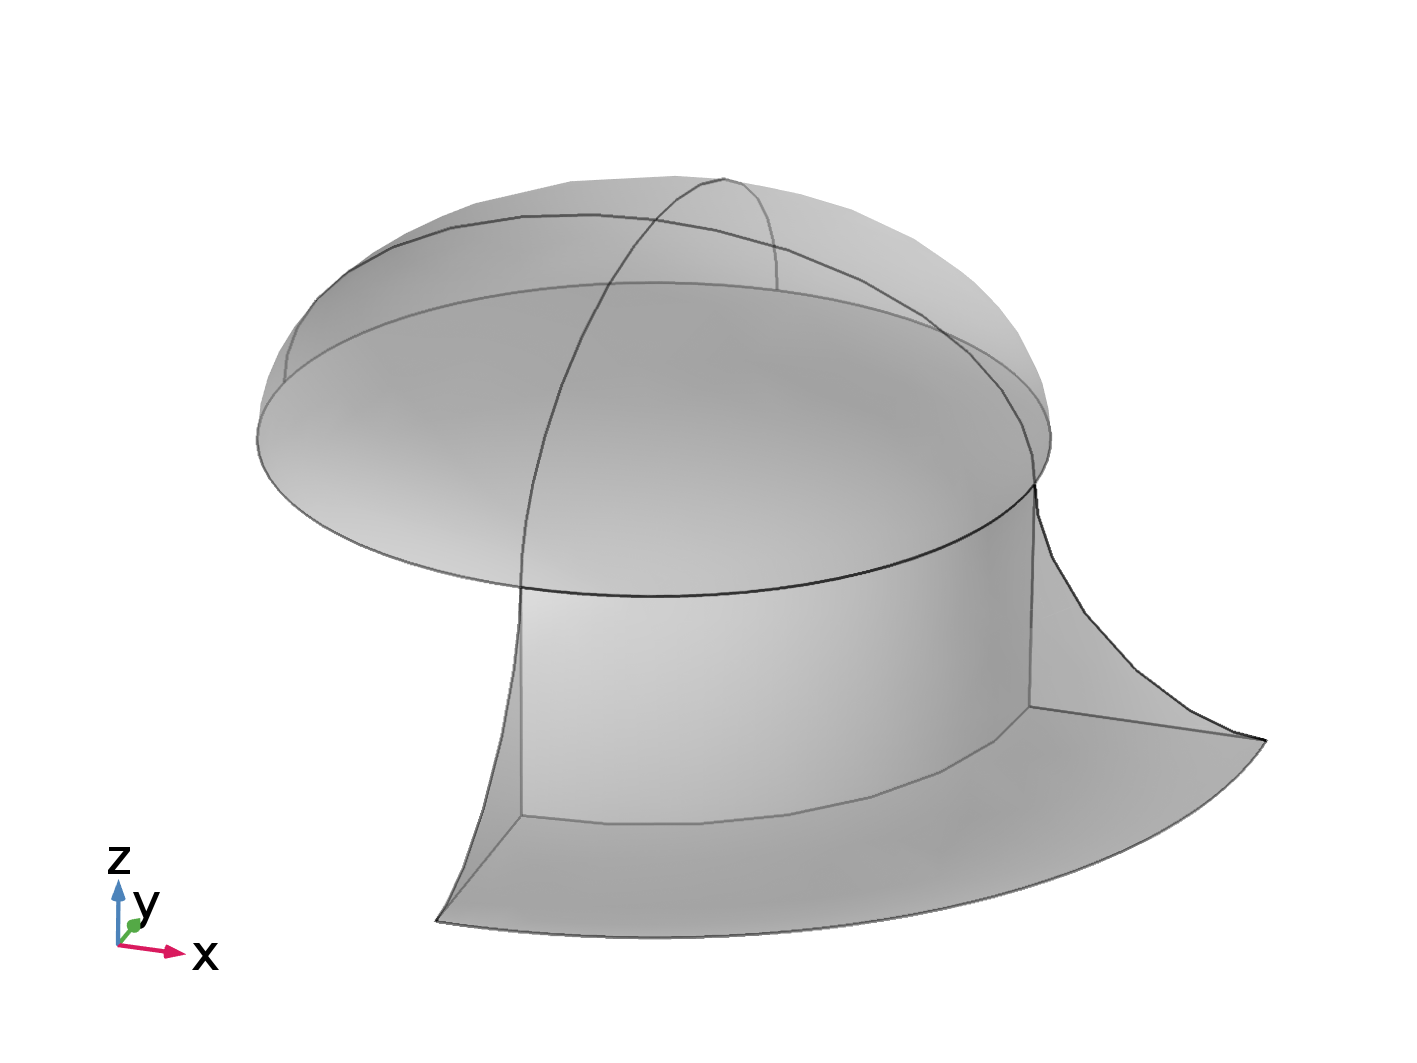
\includegraphics[width=0.8\linewidth, trim=0cm 0 0 0cm, clip]{figures/ch4/implem/geometry/Sample5A_mound_sweep.png}
    \end{subfigure}
    \begin{subfigure}{0.3\textwidth}
        \centering
        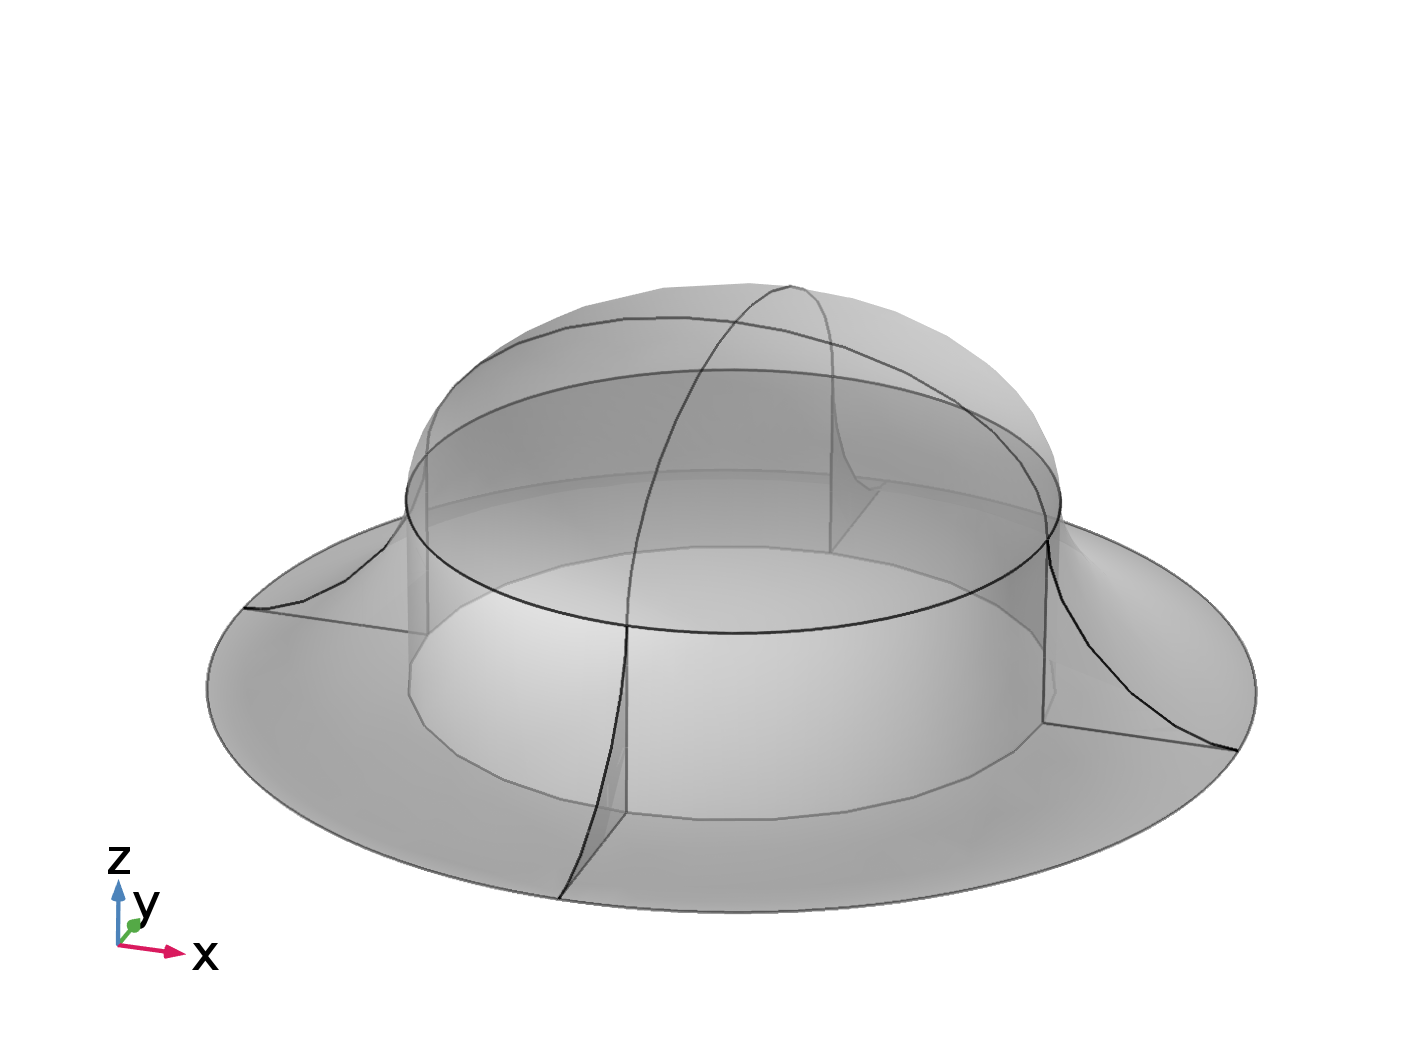
\includegraphics[width=0.8\linewidth, trim=0cm 0 0 0cm, clip]{figures/ch4/implem/geometry/Sample5A_mound_mirror2.png}
    \end{subfigure}
    \caption{The creation of the dielectric mound. The mound cross-section is defined in a workspace placed in the xz-plane, before being swept along the base of the Au particle creating a solid 3D object.}
    \label{fig:implementation_geometry_mound}
\end{figure}
\begin{figure}[htb!]
    \begin{subfigure}{0.24\textwidth}
        \centering
        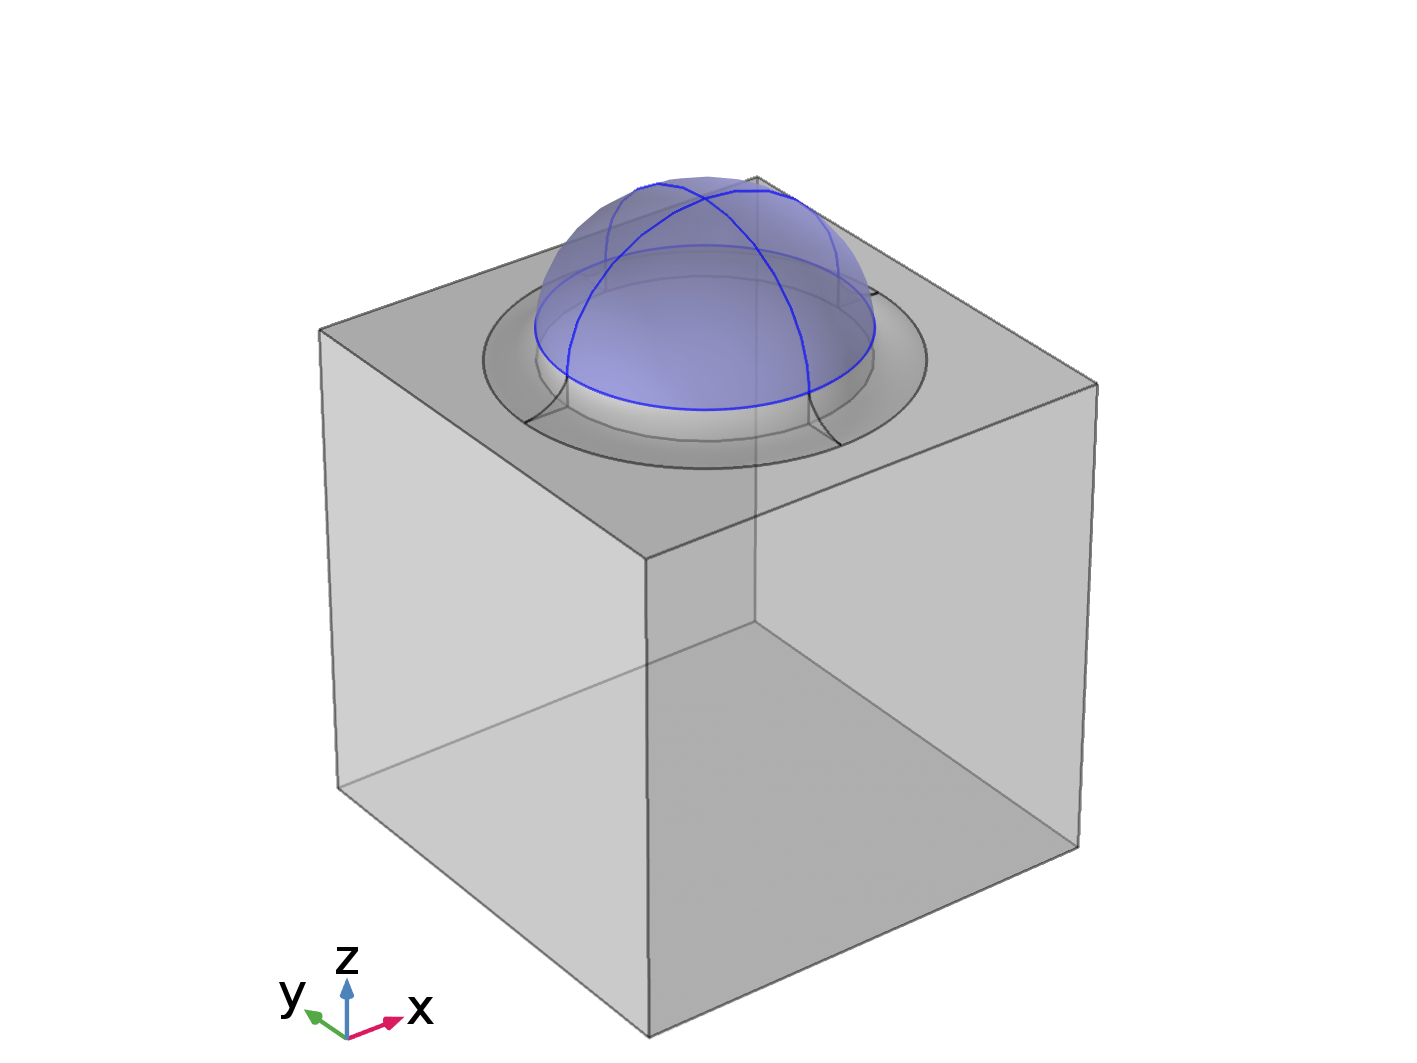
\includegraphics[width=\linewidth, trim=2cm 0cm 2cm 0cm, clip]{figures/ch4/implem/geometry/Sample6_markedAu_xyz(1).png}
        \caption{}
    \end{subfigure}
    \begin{subfigure}{0.24\textwidth}
        \centering
        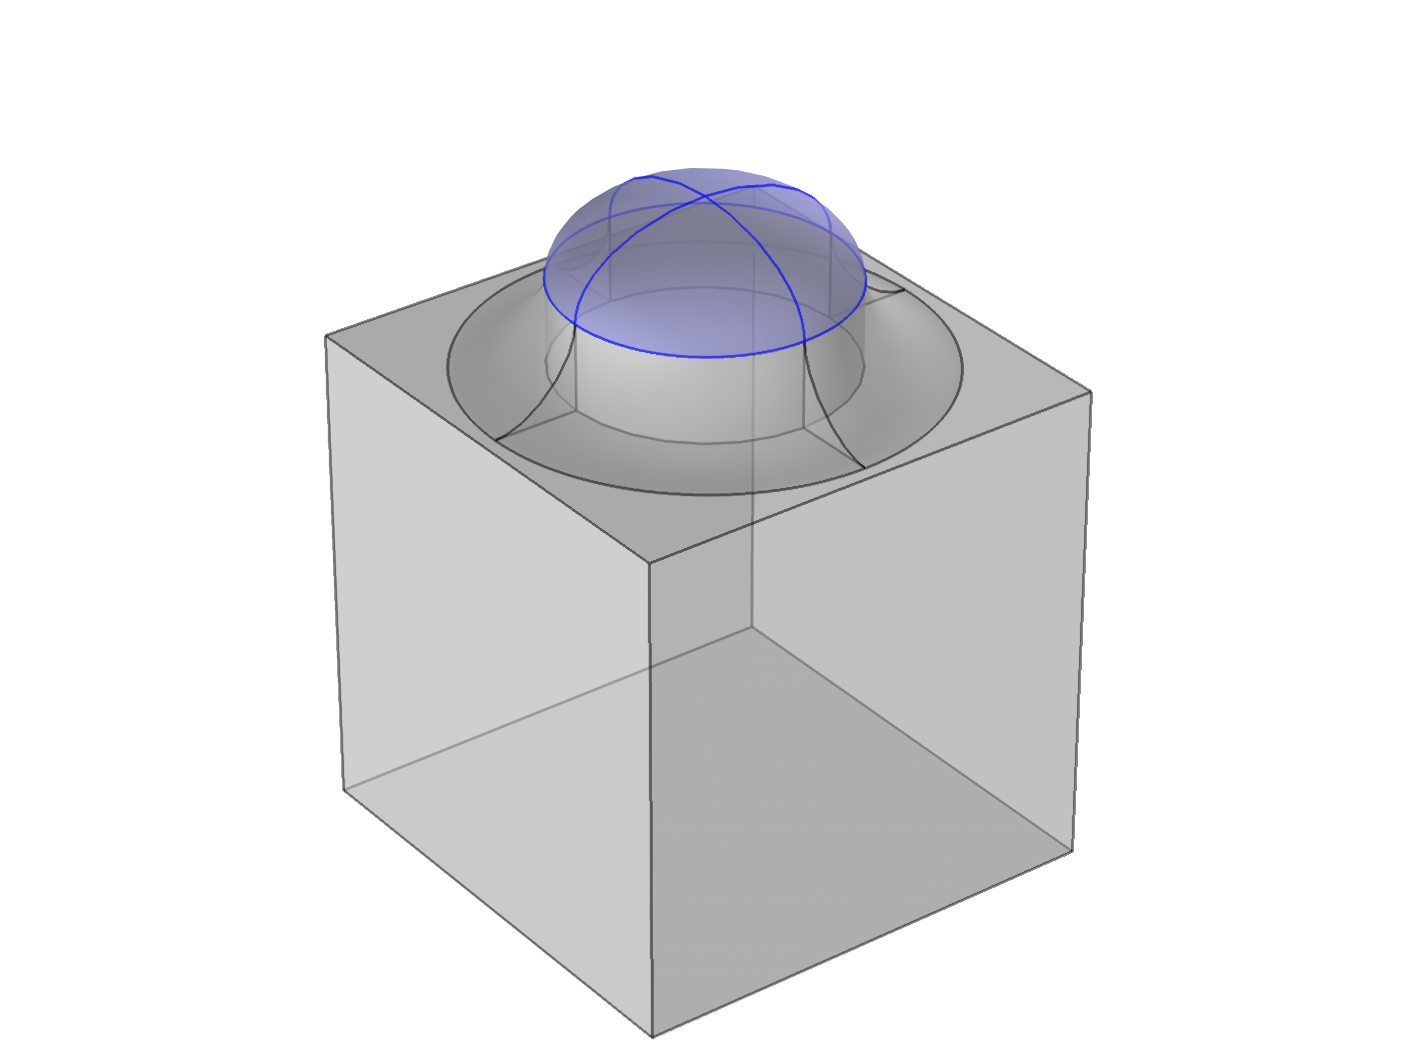
\includegraphics[width=\linewidth, trim=2cm 0cm 2cm 0cm, clip]{figures/ch4/implem/geometry/Sample5A_markedAu.png}
        \caption{}
    \end{subfigure}
    \begin{subfigure}{0.24\textwidth}
        \centering
        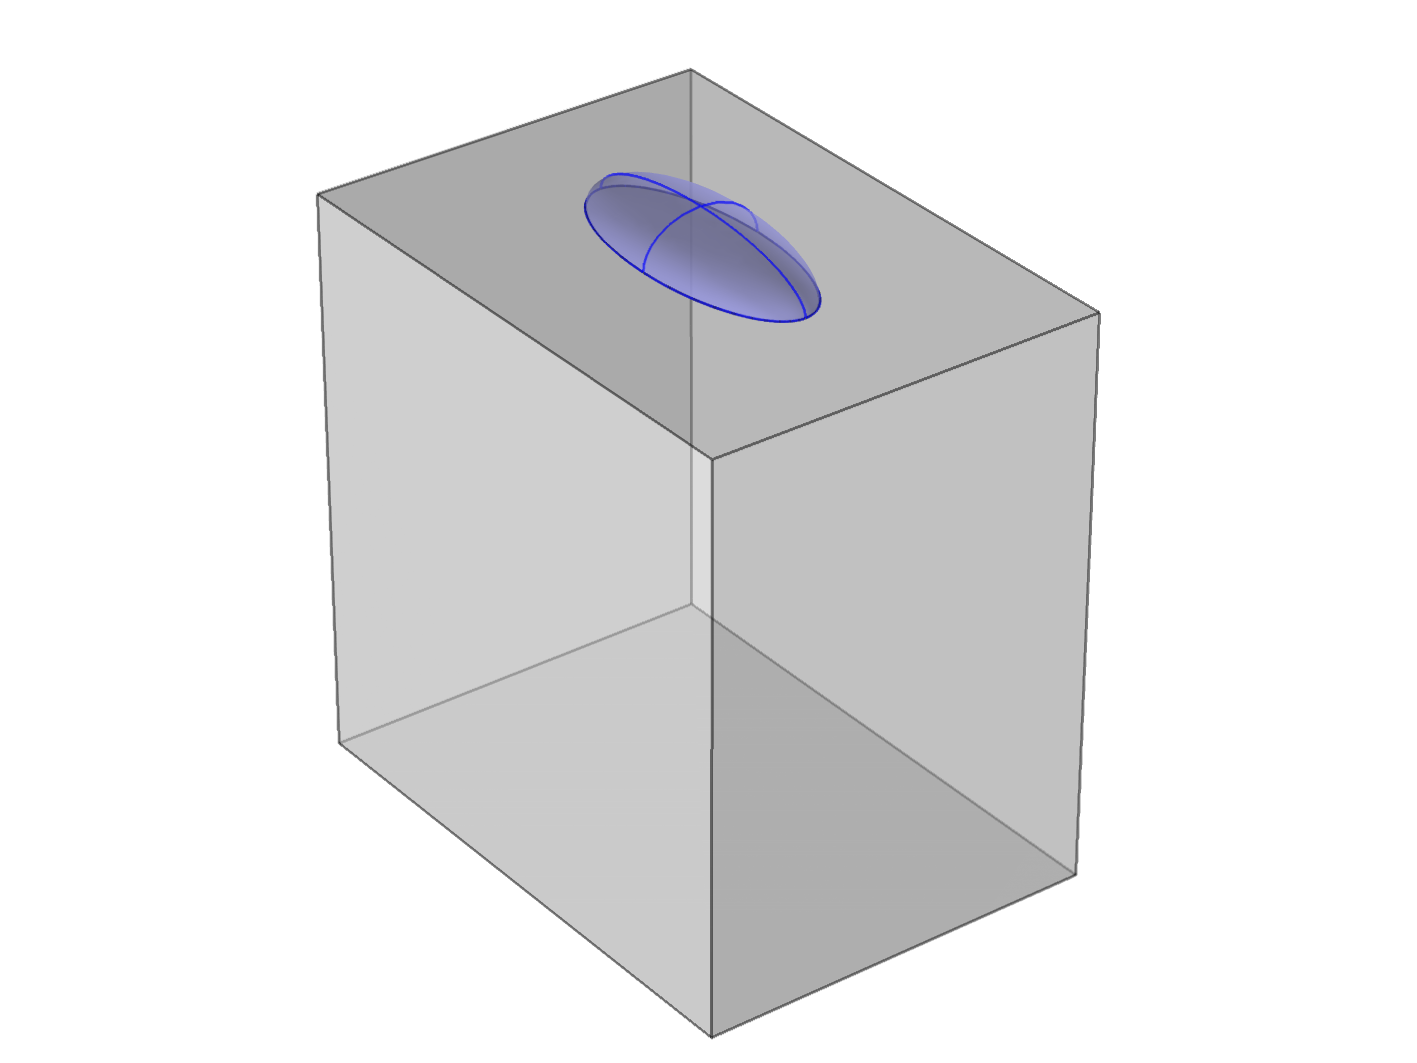
\includegraphics[width=\linewidth, trim=2cm 0cm 2cm 0cm, clip]{figures/ch4/implem/geometry/Sample5B_markedAu.png}
        \caption{}
    \end{subfigure}
    \begin{subfigure}{0.24\textwidth}
        \centering
        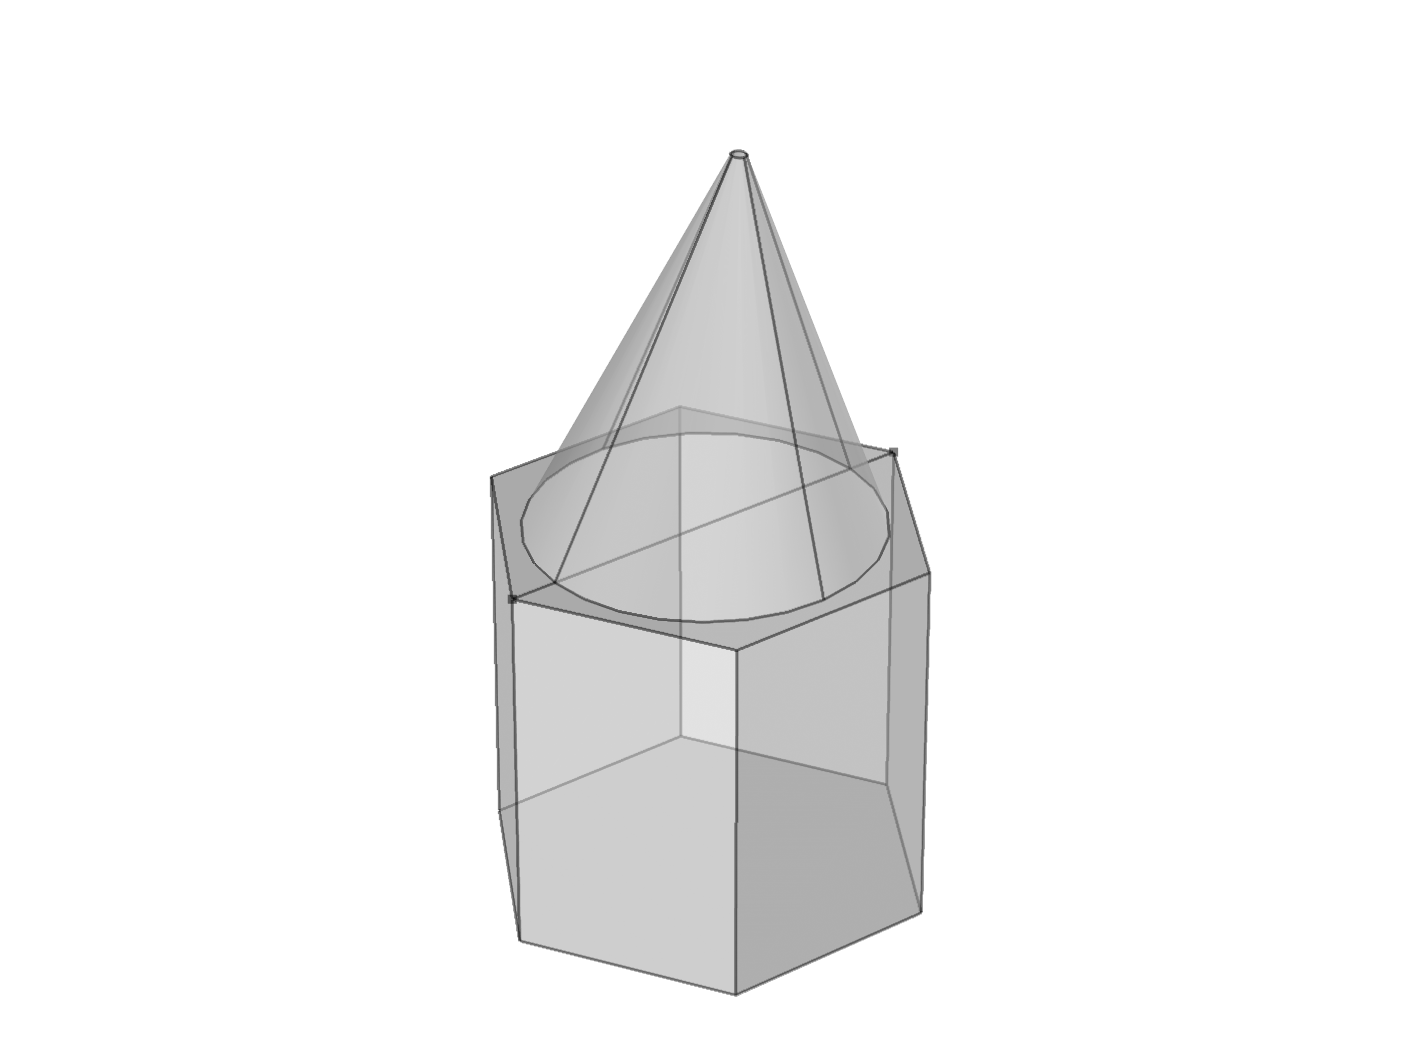
\includegraphics[width=\linewidth, trim=2cm 0cm 2cm 0cm, clip]{figures/ch4/implem/geometry/GaSb.png}
        \caption{}
    \end{subfigure}
    \caption{The physical geometries of the various periodic nanostructures implemented into COMSOL; (a) sample 6, (b) sample 5A, (c) sample 5B, and (d) tilted GaSb cones. Highlighted blue areas in (a)-(c) marks Au domains. Air domains and PMLs are hidden for improved visibility.}
    \label{fig:implementation_geometry_samples}
\end{figure}

Materials used were a dispersive SiO$_2$ and complex Au and GaSb. The refractive indices for the materials were linearly interpolated imported data tables identical to the ones used in the ellipsometric modelling of the experimental results \text{\color{red}usikker. MK: kilde til (n,k) brukt?} 

\subsection{The EWFD interface}
Two periodic ports were defined on the top boundary of the physical air domain (port 1) and bottom boundary of the substrate domain (port 2), see figure \ref{fig:implementation_ewfd_ports}. Port 1 excites an EM wave with polar AOI $\theta_0$ and azimuthal AOI $\phi_0$, while also absorbing outgoing (reflected) waves. Port 2 is a listener node, absorbing outgoing (transmitted) waves polar incident at an angle $\theta_1 = \arcsin[\sin\theta_0 n_{\text{air}}/n_{\text{sub}}(\lambda)]$ and azimuthal incidence $\phi_1=\phi_0$. Each periodic port was \text{\color{red}is?} also equipped with diffraction ports absorbing specific modes. Most notably, port 3 (top) and port 4 (bottom) read waves polarized orthogonal to the wave entering the model. The incident wave excited at port 1 is linearly polarized in either p- or s-polarization. Floquet periodicity was applied to boundaries shown in figure \ref{fig:implementation_ewfd_pc1} and \ref{fig:implementation_ewfd_pc2}

\begin{figure}[htb]
    \begin{subfigure}{0.19\textwidth}
        \centering
        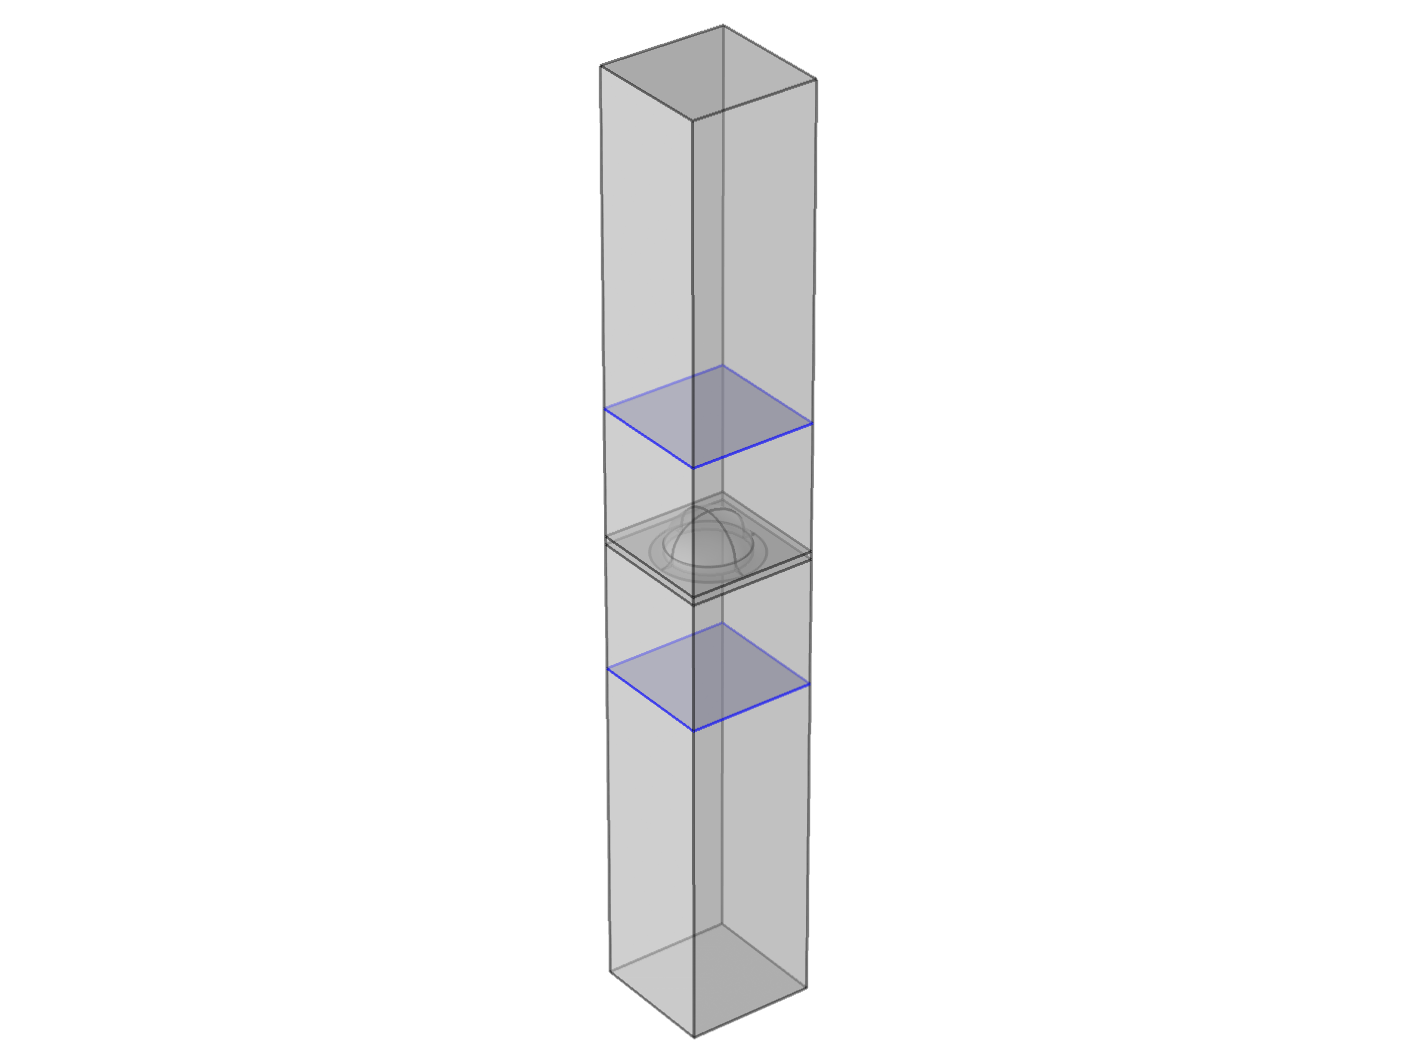
\includegraphics[width=\linewidth, trim=4.2cm 0 4.2cm 0, clip]{figures/ch4/implem/ewfd/ewfd_ports.png}
        \caption{}
        \label{fig:implementation_ewfd_ports}
    \end{subfigure}
    \begin{subfigure}{0.19\textwidth}
        \centering
        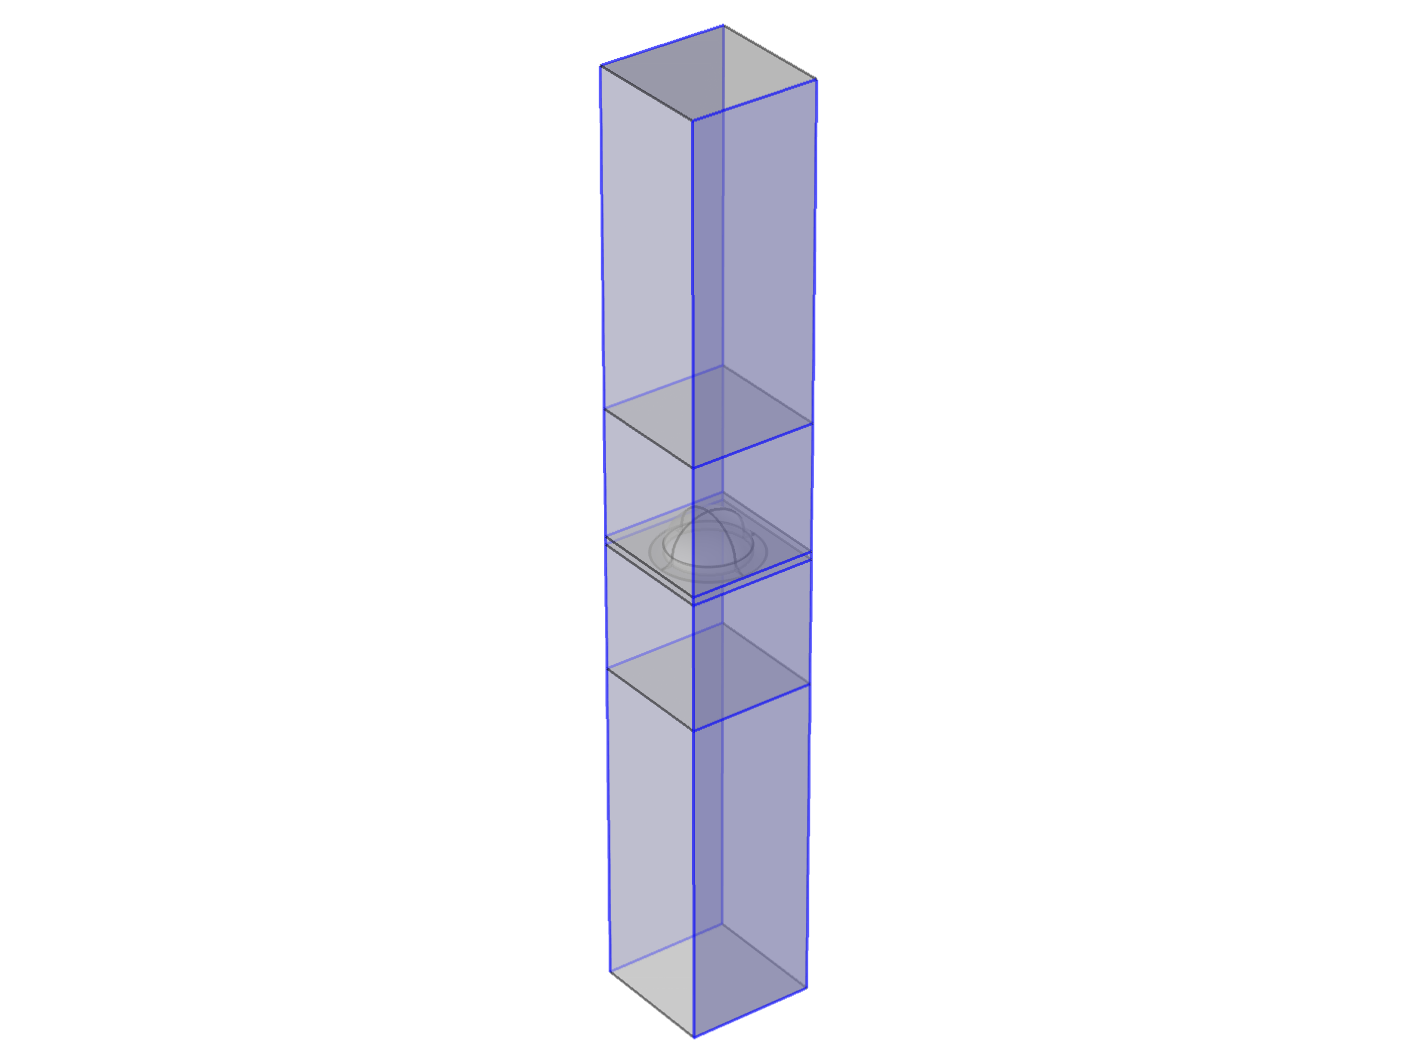
\includegraphics[width=\linewidth, trim=4.2cm 0 4.2cm 0, clip]{figures/ch4/implem/ewfd/ewfd_pc1.png}
        \caption{}
        \label{fig:implementation_ewfd_pc1}
    \end{subfigure}
    \begin{subfigure}{0.19\textwidth}
        \centering
        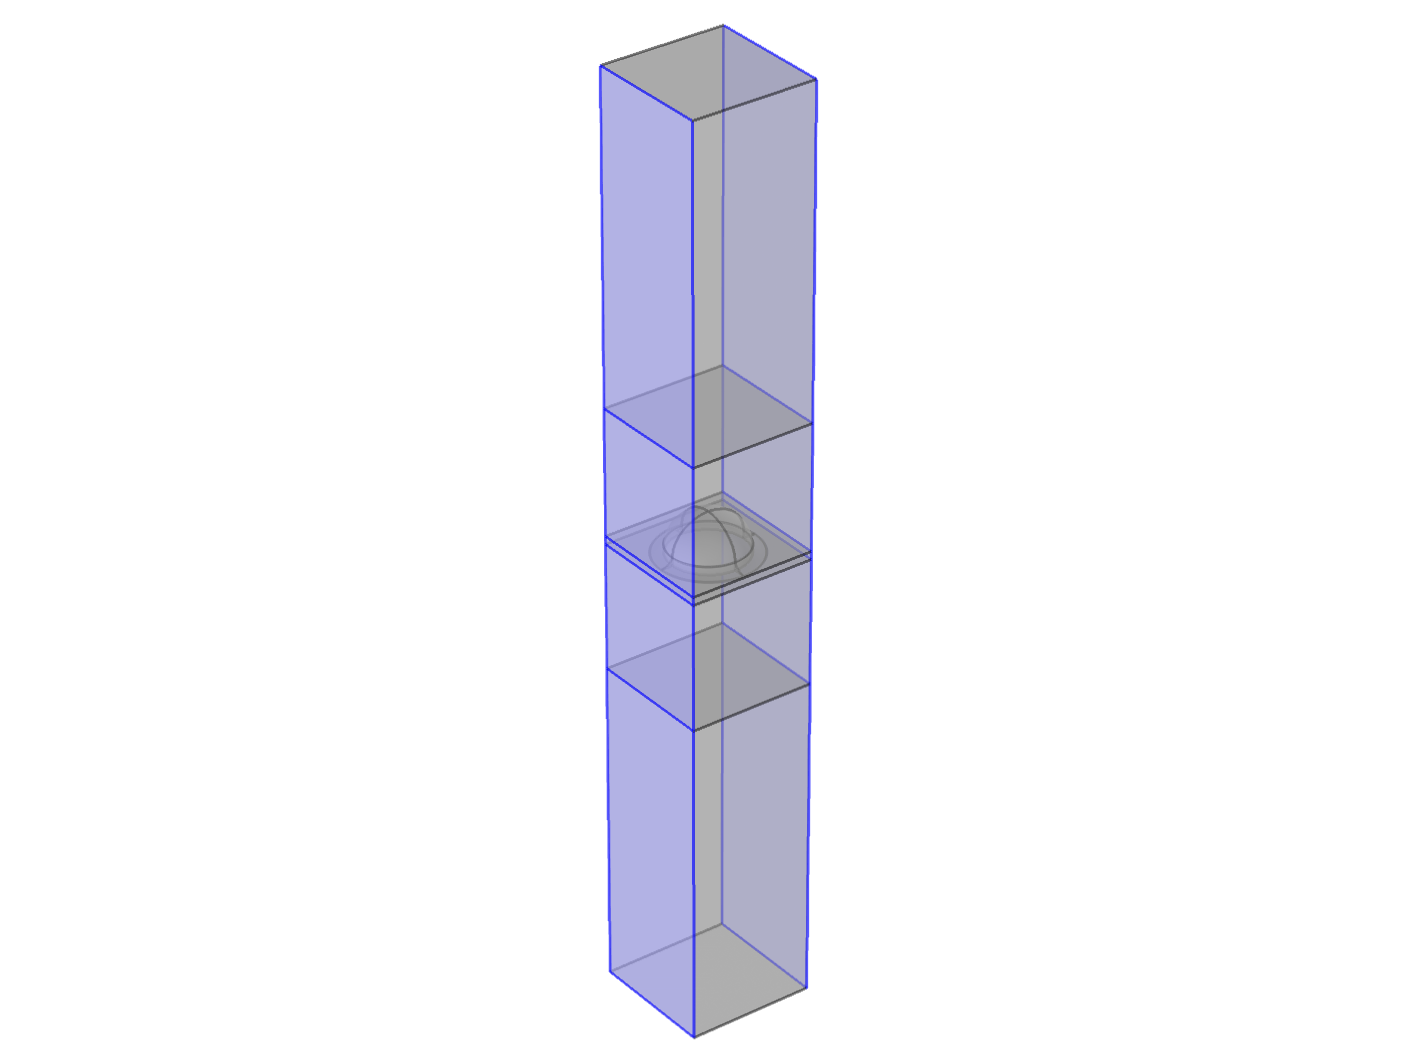
\includegraphics[width=\linewidth, trim=4.2cm 0 4.2cm 0, clip]{figures/ch4/implem/ewfd/ewfd_pc2.png}
        \caption{}
        \label{fig:implementation_ewfd_pc2}
    \end{subfigure}
    \begin{subfigure}{0.19\textwidth}
        \centering
        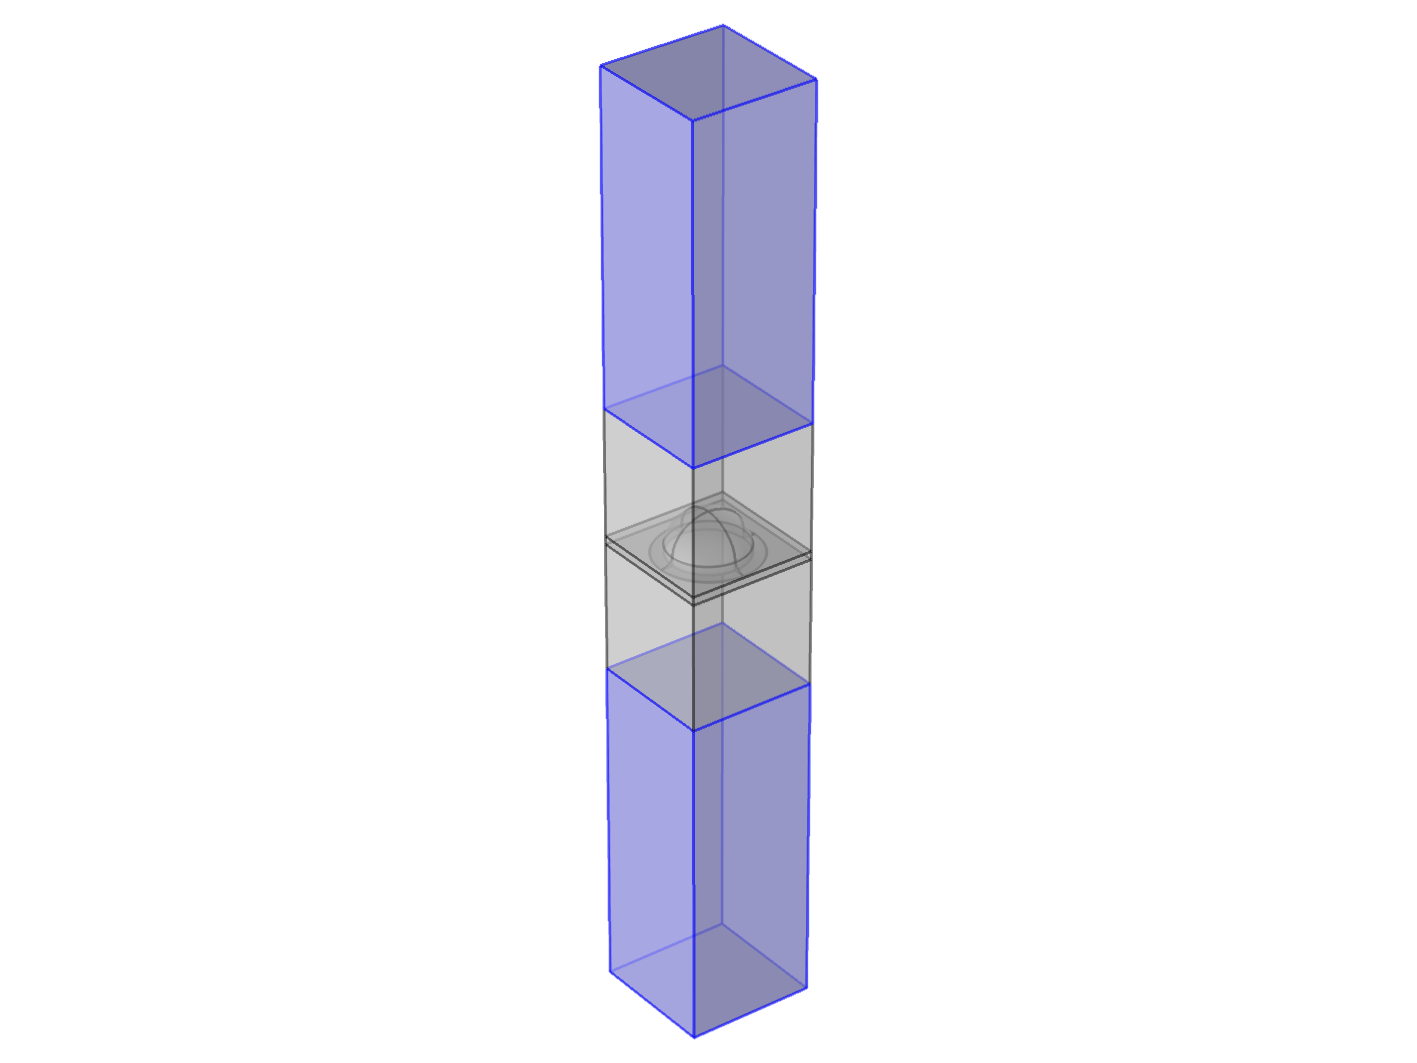
\includegraphics[width=\linewidth, trim=4.2cm 0 4.2cm 0, clip]{figures/ch4/implem/ewfd/ewfd_pml.png}
        \caption{}
        \label{fig:implementation_ewfd_pml}
    \end{subfigure}
    \begin{subfigure}{0.19\textwidth}
        \centering
        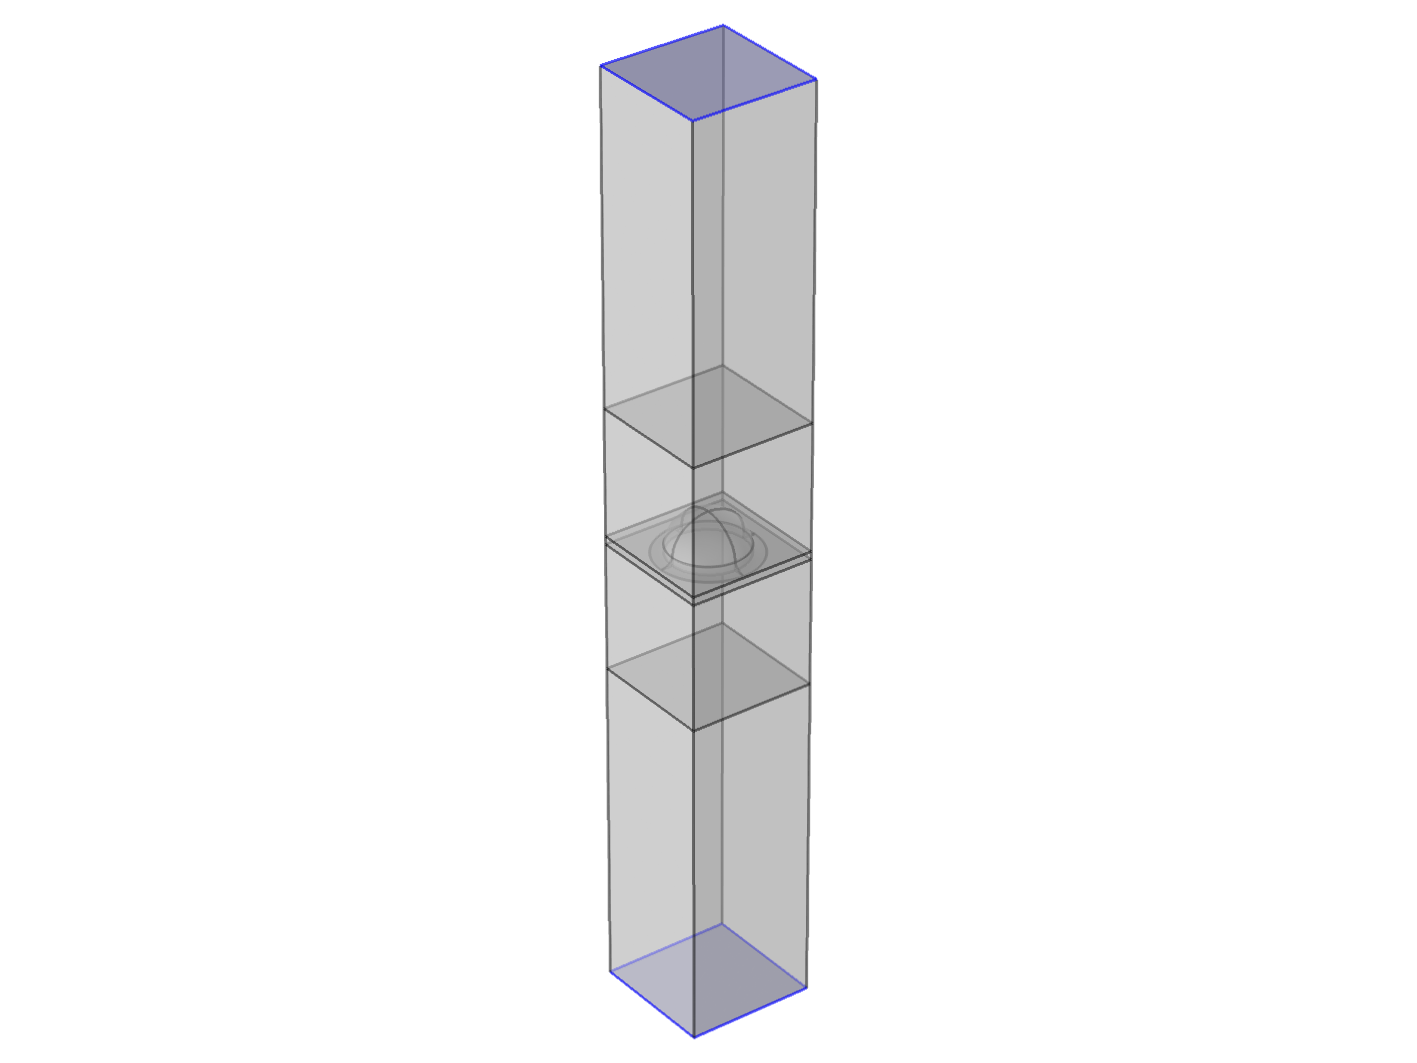
\includegraphics[width=\linewidth, trim=4.2cm 0 4.2cm 0cm, clip]{figures/ch4/implem/ewfd/ewfd_sbc.png}
        \caption{}
        \label{fig:implementation_ewfd_sbc}
    \end{subfigure}
    \caption{Setup of the EWFD interface; (a) top: port 1 and port 3, bottom: port 2 and port 4; (b)-(c) periodic boundary conditions subject to Floquet periodicity; (d) PML domains; (e) SBC boundaries.}
    \label{fig:implementation_ewfd_setup}
\end{figure}

PML domains are shown in figure \ref{fig:implementation_ewfd_pml}, while the physical domain is considered to be the volume between port 1 and 2. Because a PML region acts as an infinite open domain, any boundary conditions and material properties must be carried over to the PML region. Thus, the PML domain share the same Floquet periodicity as the physical domain as figures \ref{fig:implementation_ewfd_pc1} and \ref{fig:implementation_ewfd_pc2} shows. The upper and lower PML domains also share the refractive indices of the interior region they are adjacent to, i.e. air and substrate, respectively. First order SBC were implemented in addition to PMLs to further reduce reflection at normal incidence and was not expected to have noticeable influence on computation cost. These boundaries are shown in figure \ref{fig:implementation_ewfd_sbc}.

\subsection{Meshing}
Periodic boundaries must have compatible meshes. That is, boundary layers on opposing sides must be equal in order to properly simulate the infinite structure. Using figure \ref{fig:implementation_ewfd_pc1} as an example, the meshed boundary of the highlighted walls must be exact copies of each other, and similarly for the highlighted walls in figure \ref{fig:implementation_ewfd_pc2}. In choosing the maximum element size, a satisfactory compromise between accuracy and computational memory usage was found to be 
\begin{equation}
    \text{MES} = \frac{\lambda}{6n_i},
    \label{eq:MES=lambda/6n}
\end{equation}
where $n_i$ is the refractive index of either air, SiO$_2$, Au, or GaSb. This is further discussed in section \text{\color{red}ref: mesh convergence and wavelength dep. mesh}. 

\subsection{Study steps}
The models were solved with a parametric sweep over wavelength $\lambda$ with stepsize $\Delta\lambda=5$ nm over a wide spectrum, typically 210 nm to 1600 nm which is approximately the same as the detection range of the RC2 ellipsometer used in the experimental works. For each wavelength, a full 360 degree sweep was performed for azimuthal AOI $\phi_0$ with stepsize $\Delta\phi_0=5^{\circ}$ using a study extension called \emph{auxiliary sweep}. Auxiliary sweep uses the solution from a previous parameter as a trial function for the current parameter, thus essentially re-using a previously calculated system matrix (equation (\ref{eq:FEM_mastereq_matrix})). Being relieved the burden of assembling the system matrix for every iteration of $\phi_0$ will in principle greatly reduce the computation time compared to iterating through a regular parameter sweep where COMSOL solves the problem for each parameter from scratch. 

\text{\color{red}finner ingen kilde for dette, annet enn hva Bertil sa + forum/kommentarfelt online} %https://www.comsol.jp/blogs/solution-joining-parametric-eigenfrequency-time-dependent-problems/

\subsection{S-parameter conversion}
 The model is limited to excite only one specified polarization during the computation process. In order to derive a Jones matrix optical response and subsequently the Mueller matrix, two separate simulations must be run; one where the incident wave is p-polarized, and the other s-polarized. However, two instances of the COMSOL application may run simultaneously on the desktop computer which in practice halves the computation time. 

The complex reflection coefficients are found from waves absorbed at ports 1 and 3, i.e. S-parameters $S_{11}$ and $S_{31}$, so that
\begin{subequations} 
\begin{align}
    r_{pp} = \text{Re}[S_{11}^{(p)}] + \text{Im}[S_{11}^{(p)}]  \\
    r_{sp} = \text{Re}[S_{31}^{(p)}] + \text{Im}[S_{31}^{(p)}]  \\
    r_{ps} = \text{Re}[S_{31}^{(s)}] + \text{Im}[S_{31}^{(s)}]  \\
    r_{ss} = \text{Re}[S_{11}^{(s)}] + \text{Im}[S_{11}^{(s)}]  
\end{align}
\end{subequations}
where $S_{i1}^{(k)}$ specifies a $k$-polarized wave excited from port 1 and absorbed on port $i$. We remind the reader that the notation $r_{\alpha\beta}$ indicates conversion from $\beta$-polarization to $\alpha$-polarization after reflection. Similarly, one may find the complex transmission coefficients from ports 2 and 4,
\begin{subequations} 
\begin{align}
    t_{pp} = \text{Re}[S_{21}^{(p)}] + \text{Im}[S_{21}^{(p)}]  \\
    t_{sp} = \text{Re}[S_{41}^{(p)}] + \text{Im}[S_{41}^{(p)}]  \\
    t_{ps} = \text{Re}[S_{41}^{(s)}] + \text{Im}[S_{41}^{(s)}]  \\
    t_{ss} = \text{Re}[S_{21}^{(s)}] + \text{Im}[S_{21}^{(s)}]  
\end{align}
\end{subequations}

With the complex reflection and transmission coefficients readily available, one may find the complete Mueller matrix by equations (\ref{eq:JonesToMueller}a) - (\ref{eq:JonesToMueller}q), ellipsometry angles in equations (\ref{eq:generalized_ellipsometer_angles}a) - (\ref{eq:generalized_ellipsometer_angles}c) and the pseudo dielectric function from equation (\ref{eq:generalized_pseudo_dielectricfunction}). The COMSOL S-parameters were imported into MATLAB where these quantities were calculated and plotted.

\subsection{Joule heating}
Energy of the incident light dissipated into a material as heat can be found from equation (\ref{eq:Resistive_heating_P}) and integrating over the volume of interest. COMSOL calculates resistive heating with the integrated function 
\begin{equation}
    \texttt{ewfd.Qrh} = \frac{1}{2}\sum_i \texttt{realdot}(J_i,E_i) \quad\quad i=x,y,z
    \label{eq:Qrh_heatloss}
\end{equation}
given in SI units W$/$m$^3$, where $\texttt{realdot}(a,b)$ treat the complex numbers $a$ and $b$ as if they were real-valued vectors of length $2$ and return their dot product\cite{comsol_referencemanual}. Equation (\ref{eq:Qrh_heatloss}) resembles equation (\ref{eq:Resistive_heating_dP/dV}); heat dissipated over a volume $P_{\text{resistive}}$ is found by integrating equation (\ref{eq:Qrh_heatloss}) over a selected region, for example the gold particles as marked in figures \ref{fig:implementation_geometry_samples}a-c.

\subsection{Electric field norm}
Integrated in COMSOL is the possibility to plot certain physical quantities as functions of spatial placement in the computational domain, typically presented in cross-sections of the geometry. The electric field norm is one such quantity which is useful to visualize the distribution of the electric field. It is defined as
\begin{equation}
    \texttt{ewfd.normE} = \left [ \sum_i \texttt{realdot}(E_i,E_i) \right ]^{1/2} \quad\quad i=x,y,z
    \label{eq:normE}
\end{equation}
and given in SI units V$/$m. It can in simplified terms be considered the amplitude of the electric field, $E_\text{norm}=\sqrt{E_x^2+E_y^2+E_z^2}$. We will use the notation $E_\text{norm}$ when presenting results of equation (\ref{eq:normE}), for simplicity.
\subsection{Tilted GaSb cones \color{red}fjern?}
\label{sec:implementation_gasb_cones}


\text{\color{red}improve/move this paragraph}Previous computational models of these samples, performed using GranFilm implementation of the Bedeaux-Vlieger model, neglected finite size and retardation effects in each particle, the influence of Rayleigh/Wood anomalies, polarization coupling, and the SiO$_2$ ridge underneath each particle. A simple COMSOL model had been attempted on Sample 6, neglecting the mound geometry, which broke down for higher energies where it failed to account for diffracted modes.

%%%%%%%%%%%%%%% NEW SECTION %%%%%%%%%%%%%%%
\section{Optimization of model}
Early versions of the COMSOL models were computationally extremely demanding due to a very large amount of elements, where in most cases the computer ran out of memory before completing a simulation. Furthermore, the models did not manage to account for diffracted modes, resulting in nonsensical results in higher energy regimes. 

\label{sec:Optimization_of_model}
\begin{itemize}
    \item state of old model/no mound compared with experimental and reduced rayleigh
    \item uniform mesh vs physical mesh $=>$ improved accuracy (and computation time?)
    \item implementing PML regions $=>$ fixed UV region
    \item Decreasing height of computational region (achieving same results due to PML?) $=>$ reduce computation time and performance requirement
\end{itemize}

%%%%%%%%%%%%%%%
\subsection{Effect of PML implementation}
The height of PML domain is supposedly not a critical factor, as the equations within the PML are scaled with respect to the length of the PML. Dialog with COMSOL support suggested a PML height equal to the wavelength, but seeing as the simulations are calculated for a large spectrum, it seemed appropriate to more or less arbitrarily set it to $h_{\text{PML}}=\lambda_{\text{max}/3}$, as seen in figures \ref{fig:meshDomainHeight_c} and \ref{fig:meshDomainHeight_d}. \text{\color{red}kjedelig/unødvendig avsnitt?}

\begin{itemize}
    \item before/after comparison 
    \begin{itemize}
        \item Result accuracy
        \item Computation time
        \item Memory usage
    \end{itemize}
\end{itemize}

\begin{figure}[htb]
    \centering
    \begin{subfigure}{.2\textwidth}
        \centering
        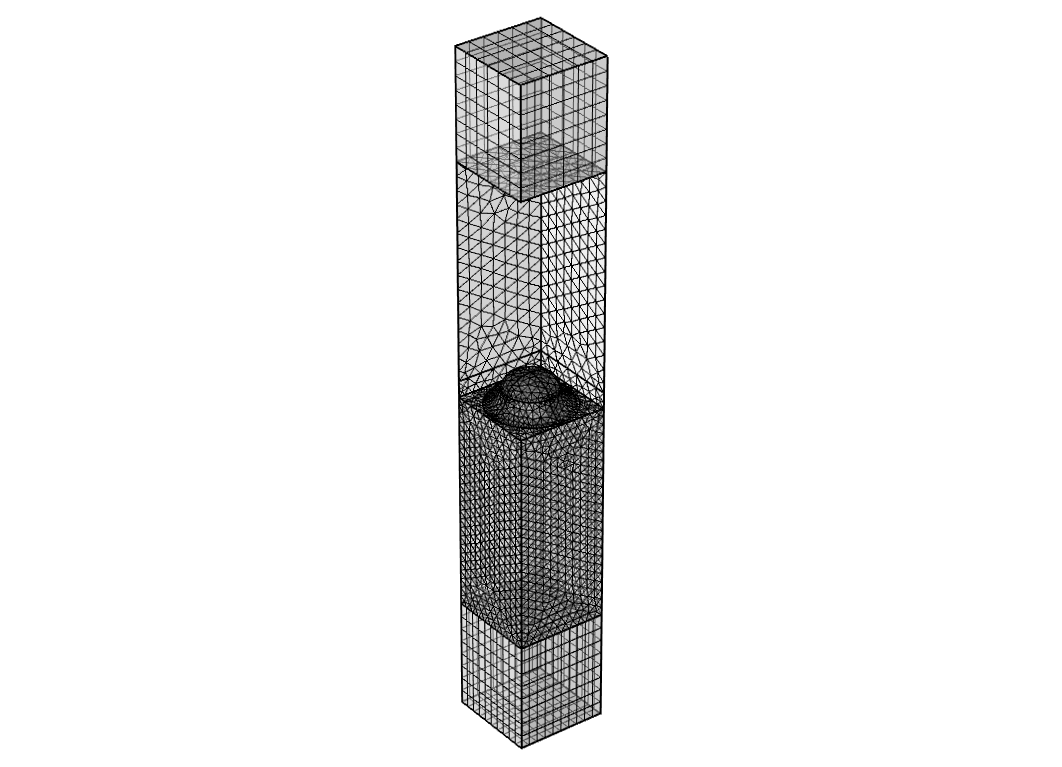
\includegraphics[scale=0.4, trim=12cm 0cm 12cm 0cm, clip]{figures/ch4/Mesh_210nm_hair=hsub=500_PMLheight=250_current.png}
        \caption{$\lambda=210$ nm}
        \label{fig:meshDomainHeight_a}
    \end{subfigure}%
    \begin{subfigure}{.2\textwidth}
        \centering %width=.8\linewidth
        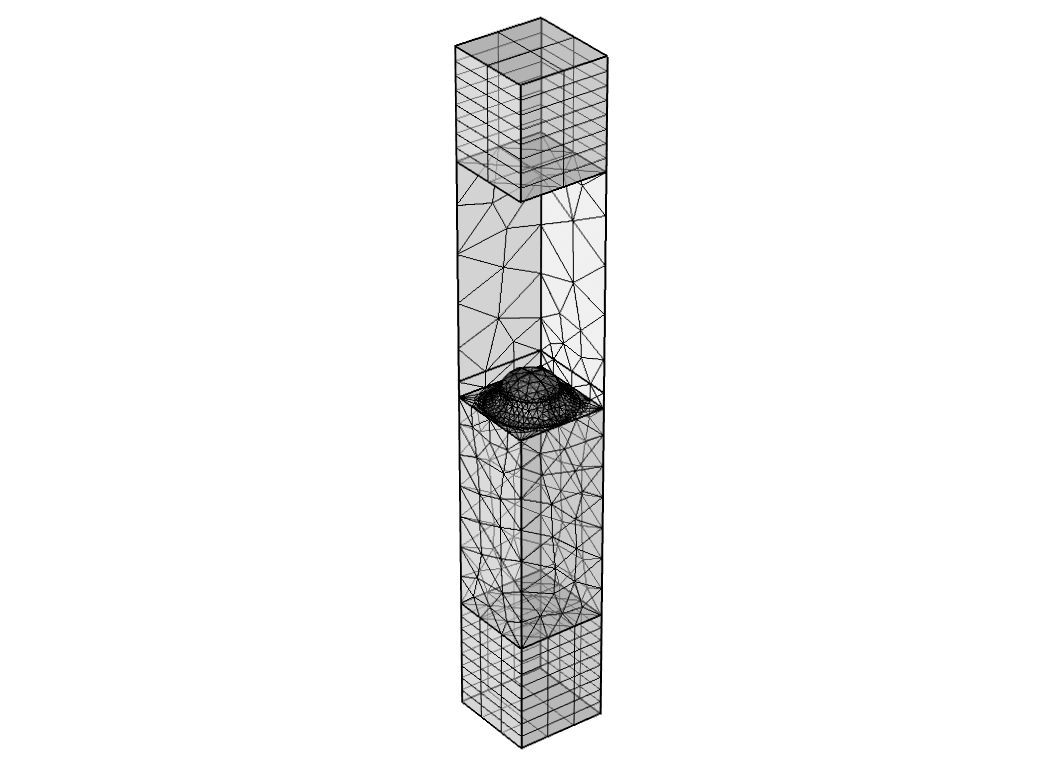
\includegraphics[scale=0.4, trim=12cm 0cm 12cm 0cm, clip]{figures/ch4/Mesh_800nm_hair=hsub=500_PMLheight=250_current.png}
        \caption{$\lambda=800$ nm}
        \label{fig:meshDomainHeight_b}
    \end{subfigure}
    \begin{subfigure}{.2\textwidth}
        \centering %width=.8\linewidth
        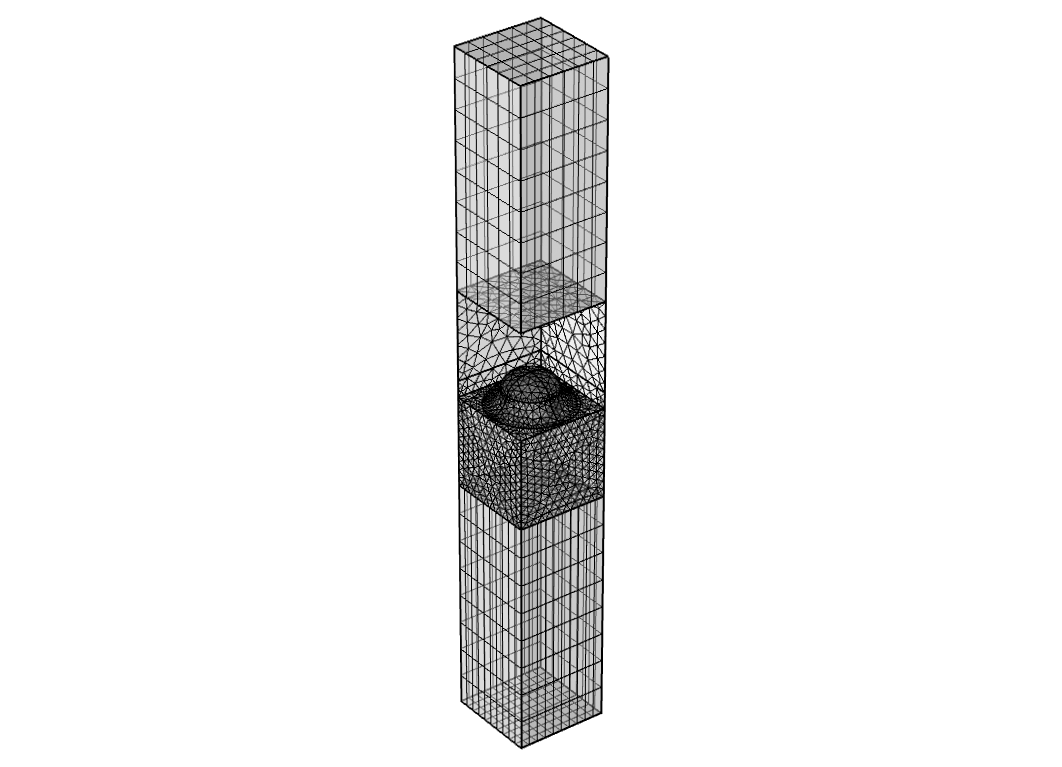
\includegraphics[scale=0.4, trim=12cm 0cm 12cm 0cm, clip]{figures/ch4/Mesh_210nm_hair=hsub=ax_PMLheight=033wl_max_wl_max=1600_current.png}
        \caption{$\lambda=210$ nm}
        \label{fig:meshDomainHeight_c}
    \end{subfigure}
    \begin{subfigure}{.2\textwidth}
        \centering %width=.8\linewidth
        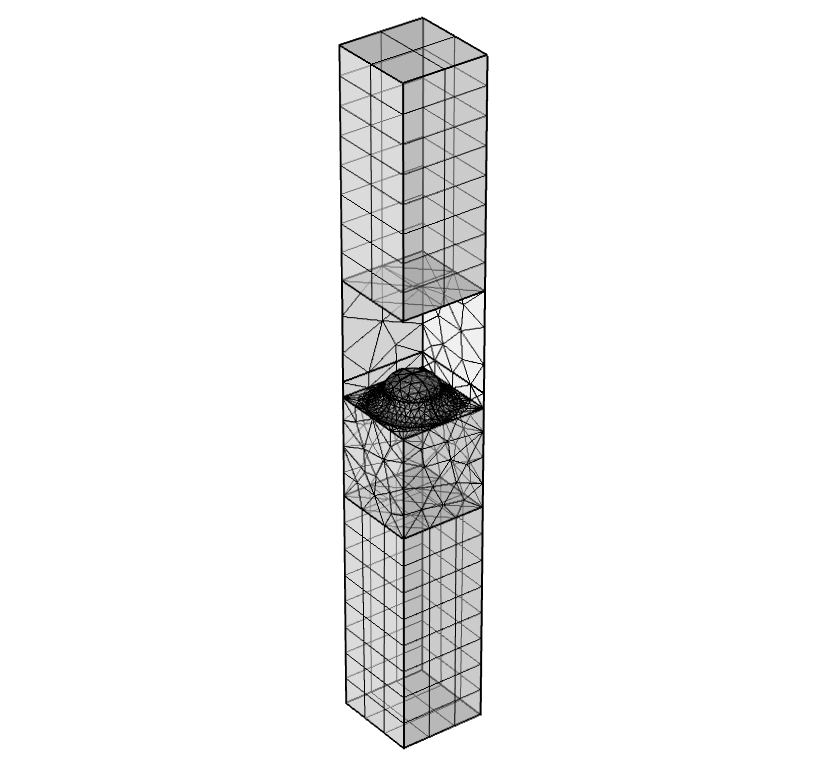
\includegraphics[scale=0.4, trim=8cm 0cm 8cm 0cm, clip]{figures/ch4/Mesh_800nm_hair=hsub=ax_PMLheight=033wl_max_wl_max=1600_current.png}
        \caption{$\lambda=800$ nm}
        \label{fig:meshDomainHeight_d}
    \end{subfigure}
    \caption{Distribution of mesh elements for different wavelengths and geometry parameters for sample 5A. In (c)-(d) the distance from the top of the gold particle to PML (and, thus, also the port) is reduced to be the same as the lattice constant. Meanwhile, the height of PML region is increased to $h_{\text{PML}}=\lambda_{\text{max}}/3$. Number of mesh elements for each are shown in Table \ref{tab:domainHeight}. Note from inspection that the number of PML elements remain the same from (a) to (c), and from (b) to (d). Outer walls of air domain are hidden for clarity.}
    \label{fig:meshDomainHeight}
\end{figure}

%%%%%%%%%%%%%%%
\subsection{Meshing Improvements}
\label{sec:optimization_mesh}
\subsubsection{Physics dependent mesh}
Early models meshed the computational domain indiscriminately, resulting in an extremely fine resolved mesh distributed equally throughout the volume and thus a very large amount of finite elements. Later versions made the mesh dependent on the refractive index. In figure \ref{fig:meshDomainHeight_a} one can see that the air domain has slightly coarser mesh than the glass substrate, while the Au particle is even more detailed due to the higher refractive index of gold, but also due to the curvature of the geometry. 

At first, models with this element size configuration used the same mesh throughout the simulation. The mesh would then be built with regards to the smallest wavelength, $\text{MES}=\lambda_{\text{min}}/(6n)$, where in most cases $\lambda_{\text{min}}=210$ nm. The mesh would look like figure \ref{fig:meshDomainHeight_a} for all wavelengths, meaning that for the vast majority of iterations the simulation is computed for an unnecessarily detailed mesh. A dynamic meshing system was introduced which rebuilt the mesh every iteration of wavelength, so that longer wavelengths use coarser mesh while still being able to properly resolve the wave. Figure \ref{fig:meshDomainHeight_b} exemplifies this for $\lambda=800$ nm. This implementation has significant impact on computation time, see table \ref{tab:domainHeight} for the real-time computation of the meshes seen in figure \ref{fig:meshDomainHeight}. 

The new setup also included the option of rebuilding the mesh less frequently, which is useful in cases where generating a new mesh every wavelength iteration is computationally demanding and time consuming.

\begin{figure}[h]  %% GaSb Computation time & #elements %% 
    \begin{subfigure}{0.49\textwidth}
        \centering
        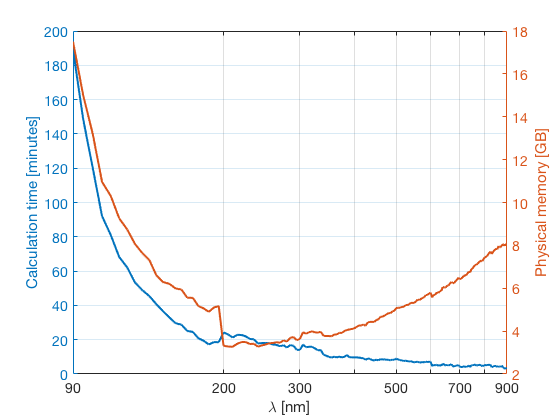
\includegraphics[width=\linewidth]{figures/ch4/gasb/ComputationTime_GaSbCones_wl90-900_phi0-355_log.png}
        \caption{}
        \label{fig:GaSb_comptimeb}
    \end{subfigure}
    \begin{subfigure}{0.49\textwidth}
        \centering
        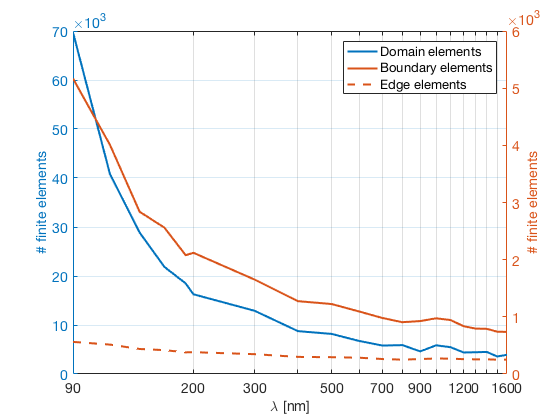
\includegraphics[width=\linewidth]{figures/ch4/gasb/Elements_vs_wavelength_log.png}
        \caption{}
        \label{fig:GaSb_comptimea}
    \end{subfigure}
    \caption{Computer performance in calculation of the tilted GaSb cones, where each iteration of wavelength (stepsize 5 nm) includes an auxiliary parametric sweep of azimuthal rotation $\phi_0$ valued from $0^\circ$ to $355^\circ$ (stepsize $5^\circ$).  (a) Calculation time (in minutes) as well as amount of physical memory used (unit in gigabytes) at a given wavelength iteration. Incident wave is TE polarized. (b) Number of elements at a given wavelength iteration. }
    \label{fig:GaSb_comptime}
\end{figure}
Computation time for each wavelength iteration increases exponentially with decreasing wavelength. This is best shown in the model of GaSb cones, as it is simulated for wavelengths down to 90 nm. Figure \ref{fig:GaSb_comptime} shows logarithmic plots of calculation time and memory usage as a function of wavelength, as well as the number of elements the mesh consists of at a given wavelength, illustrating how computation time is dependent on the amount of finite elements to solve. Due to the simulation being computationally demanding, it had to be split into smaller segments where each segment (run separately) calculated their own region of wavelength. The sharp changes at 200 nm and 900 nm is where one segment is finished and another begins. This is further explained in section \ref{sec:results_gasb}. In the GaSb cone model, the number of elements seem to stagnate around 700 nm, suggesting that it is unnecessary to further update the mesh beyond this point, as it would not result in fewer elements to solve in order to reduce computation time.

The exponentially decreasing computation time with increasing wavelength seen in figure \ref{fig:GaSb_comptime} is a trend common for all the samples simulated. It is clear that implementing a physics dependent mesh has an extreme effect on the total computation time for each simulation. With it, the TE simulation for the GaSb cones were completed in 2 days and 2 hours, whereas the same simulation running for a constant mesh configured for the lowest wavelength would take almost 40 days to complete!
%Judging from figure REFa, it was seen sufficient to update the mesh only every 300 nm, at 900nm, 1200nm and 1500nm when doing calculations above . 


%\text{\color{red}Skriv om eller fjern hele denne delen om antall elements}

%[when discussing time/memory usage] As I was forced to run the simulation into two parts (200-900 nm and 905-1600 nm), different stepsize in mesh-update was used. The former updated mesh for every new iteration of wavelength (every 5 nm) while the latter updated the mesh every five iteration (every 300 nm). It was seen as unnecessary to update the mesh as often for longer wavelengths, as the coarseness of the mesh will stagnate; even though the wavelengths are much larger than the size of the unit cell (e.g. 1600 nm wavelength vs ~40 nm unit cell) COMSOL requires the mesh to have a minimum level of detail in order to resolve the geometry. 

%\text{\color{red}{fjern eller rediger}}
%At 900 nm, the number of domain elements for a mesh with maximum element size of $\lambda/6$ is 4612 (926 boundary elements. Comp time 3mins 0-355 degrees), while the mesh at 200 nm has 16270 (2120 boundary elements. Comp time 24mins 0-355 degrees.). At 1600 nm, however, the mesh consists of 3923 boundary elements (736 boundary elements. Comptime ?), hardly any fewer than the starting point at 900 nm. I.e. the time saved in re-building a coarser mesh during the latter region of 900-1600nm and calculating a (slightly) lower number of elements is not as favourable as the higher energy region.

\subsubsection*{Reducing volume of computational domain}

Throughout most of the thesis work the height of physical domain remained a constant 1000 nm for most simulations as seen in figures \ref{fig:meshDomainHeight_a} and \ref{fig:meshDomainHeight_b}, so that the distance from the point of reflection to ports were comparable to the wavelength. Reducing the size of this domain without affecting accuracy of results would greatly improve computational performance.

When using domain-backed ports as here\footnote{The ports are backed by the PML domains, see figures \ref{fig:implementation_ewfd_ports} and \ref{fig:implementation_ewfd_pml}.}, the port locations does not matter \text{\color{red}[source: COMSOL support...]} and should correctly extract the plane-wave component from the field regardless of distance. However, the distance to the PML domains \emph{does} matter. PMLs do not dampen evanescent diffraction orders, so that these must decay before reaching the PML\cite{PML_reflectionOfEvanescentWaves1}\cite{PML_reflectionOfEvanescentWaves2}. The decay length of the evanescent waves are given by equation (\ref{eq:decaylength_grating}), and for sub-wavelength nanostructures the criterion for neglecting evanescent wave-coupling with the PMLs becomes $h_{\text{air, sub}}\gg a_{x,y}/(2\pi)$, where $h_{\text{air, sub}}$ is the height of the air or substrate domain (\text{\color{red}fjern hvis introdusert tidligere}) and  $a_{x,y}=\text{max}(a_x,a_y)$ is whichever lattice constant is the largest for the sample\cite{decaylength_comsolsupport}. A more practical criterion for the minimum distance from reflection point to PML is then 
\begin{equation}
    h_{\text{air, sub}}> \frac{a_{x,y}}{2},
    \label{eq:height_physicaldomain}
\end{equation}
for nanostructures with periodicity smaller than the wavelength\cite{decaylength_comsolsupport}. In the thesis COMSOL models, the distance from the base of the Au or GaSb particles ($z=0$) to the top port ($z=h_{\text{air}}$) was set to
\begin{subequations}
\begin{equation}
    h_{\text{air}} = a_{x,y} + R_z
\end{equation}
for the gold hemispheroidal samples, and
\begin{equation}
    h_{\text{air}} = d + h
\end{equation}
\end{subequations}
for the tilted GaSb cones. Distance to bottom port was set equal to $ h_{\text{air}}$, except for the GaSb model where it was halved, $h_{\text{sub}} = h_{\text{air}}/2$, due to the absorptive nature of the GaSb substrate.

As seen in figure \ref{fig:meshDomainHeight} and table \ref{tab:domainHeight}, reducing the volume of the physical domain drastically reduce the amount of elements to solve and hence reduces the required amount of RAM and computation time, particularly at lower wavelengths. Without this volume reduction some of the sample results to be presented would not be possible to calculate, considering that certain simulations pushed the limits of the desktop computer even after reducing the computational domain (specifically the GaSb cones), 
%Because samples 6, 5A and 5B vary a great deal in size, and it was desirable for the models to be effortlessly interchangeable by changing only the sample parameters, the actual height of ambient and substrate domains used in the final model was
%\begin{equation}
%    h_{\text{air, sub}} = a_{x,y} + R_z
%\end{equation}
%for the gold hemispheroidal models, and
%\begin{equation}
%    h_{\text{air, sub}} = d + h
%\end{equation}
%for the tilted GaSb cones model, where $d$ is the inter-cone distance and $h$ the vertical height of the tilted cone.

 \begin{table}[htb!]
    \centering
    \caption{Performance differences when comparing size of computational volume and wavelengths for sample 5A. Computation time and memory usage is tracked for a single wavelength TE wave at one fixed angle of incidence $\phi_0=0^\circ$. Fixed volume: constant height for air and substrate domains $h_{\text{air}}=h_{\text{sub}}=500$ nm regardless of sample parameters, as well as fixed PML height of half the size of air domain. Reduced volume: height of computational domain is equal equation (\ref{eq:hei}). From left to right, each column correspond to figure \ref{fig:meshDomainHeight}a-d.}
    \label{tab:domainHeight}
    \begin{tabular}{l l l l l}
    %       &   Fixed \par volume   &            &   Reduced volume  &     \\
    & \multicolumn{2}{c}{Fixed volume} & \multicolumn{2}{c}{Reduced volume} \\
            &   @ 210 nm    &  @ 800 nm    &  @ 210 nm        & @ 800 nm \\
    \hline 
    $\#$ domain elements    &   49 587      &   8 089       &   28 249      &   7 741\\
    $\#$ boundary elements  &   6 028       &   2 197       &   4 432       &   2 055\\
    $\#$ edge elements      &   602         &   356         &   522         &   328\\
    Physical memory         &   9.94 GB      &   2.13 GB      &   6.26 GB      &   1.91 GB\\
    Computation time        &   71 s    &   6 s          &   36s          &   6 s\\ %1min11s=71s
    \hline
    \end{tabular}
\end{table}


In conclusion, all the above-mentioned changes to the COMSOL model has improved accuracy in results (especially higher energies where diffracted modes occur), greatly decreased  computational cost on memory\text{\color{red}husk: den første modellen kunne knapt kjøre S6 pga utløpt minne}, and reduced computation time, particularly when computing lower wavelengths.



\subsubsection*{Mesh convergence tests}
As stated in equation (\ref{eq:MES=lambda/6n}), the maximum element size was decreased to a factor 1/6 for improved confidence in results. Convergence tests were also done with mesh factor 1/8, however, the extra cost of computation time and memory usage greatly outweighed the slight increase in accuracy. A convergence limit appeared to be approached already at factor 1/5 (see Appendix \ref{sec:AppendixA}, figure \ref{fig:AppendixConvergence}), so a factor 1/6 was deemed to be adequate enough.
\text{\color{red}FIGUR}




    Mesh convergence. Fix plot av "error on approximation on coarser meshes", $e=u_{h2}-u_{h1}$ der 1 og 2 representerer to ulike mesh instillinger e.g. $\lambda/5$ vs $\lambda/6$ %https://www.comsol.com/multiphysics/finite-element-method#discret1

%%%%%%%%%%%%%%% NEW SECTION %%%%%%%%%%%%%%%
%\section{Verification of model by analytic test equations}
%\improvement{Improve title}
%\text{\color{red}flytt section til appendix?}
%\info{results of hexagonal lattice in appendix}
%\begin{itemize}
%    \item Fresnel equations on air/glass interface, constant refractive indices. 
%    \item error estimate $e=R_{analytic}-R_{COMSOL}$
%\end{itemize}

%%%%%%%%%%%%%%% NEW SECTION %%%%%%%%%%%%%%%
\section{Sample 6}
Sample 6 was first simulated with a fixed height of the computational domain, similar to figures \ref{fig:meshDomainHeight}a-b. At a polar AOI $\theta_0=55^\circ$ for the wavelengths $\lambda=210-1200$ nm and azimuthal AOI $\phi_0=0^\circ-360^\circ$, the total elapsed real-time it took to complete the COMSOL simulation (also known as the \emph{wall time}) was 312 hours and 35 minutes, including both TE and TM simulations. However, these two were running simultaneously on the same computer, effectively reducing the actual time spent by half. By default, COMSOL uses the total number of available physical CPU cores during calculations. Assuming that the code is well balanced in that each core does approximately the same amount of work, the \emph{CPU time} using COMSOL can be estimated as the wall time multiplied by the amount of physical cores. In this case the CPU time becomes 78 days, 3 hours and 30 minutes! At a later stage, the simulations were run again for a reduced height of the computational domain similar to figures \ref{fig:meshDomainHeight}c-d, which reduced the wall time to approximately 82 hours without affecting accuracy of the results. On average, this is about 10 seconds wall time per wavelength per azimuthal angle.

\begin{figure}[h]  %% Rpp & Rss contour E and phi
    \begin{subfigure}{0.49\textwidth}
        \centering
        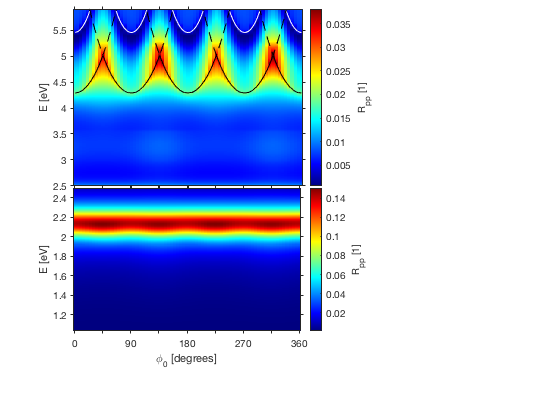
\includegraphics[width=0.99\linewidth, trim=1.1cm 1.8cm 6.7cm 0.3cm, clip]{figures/ch4/S6/contour/S6_Rpp.png}
        \caption{}
        \label{fig:S6_contour_Rpp}
    \end{subfigure}
    \begin{subfigure}{0.49\textwidth}
        \centering
        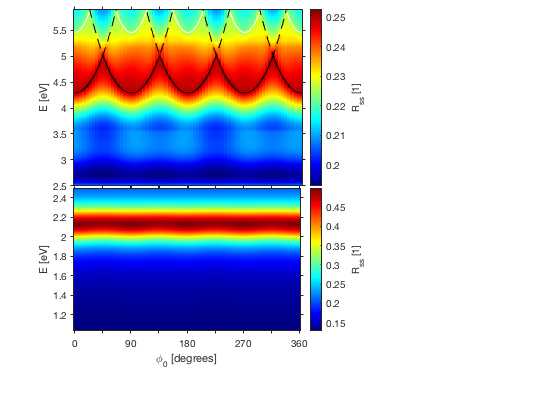
\includegraphics[width=0.99\linewidth, trim=1.1cm 1.8cm 6.7cm 0.3cm, clip]{figures/ch4/S6/contour/S6_Rss.png}
        \caption{}
        \label{fig:S6_contour_Rss}
    \end{subfigure}
    %\caption{}
    %\label{fig:S6_contour_Rpp&Rss}

    \begin{subfigure}{0.49\textwidth}
        \centering
        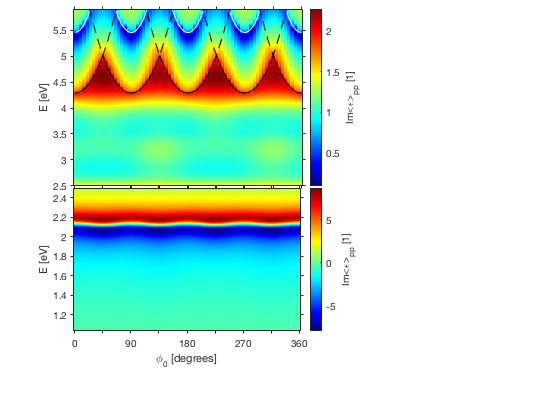
\includegraphics[width=0.99\linewidth, trim=1.1cm 1.8cm 6.7cm 0.3cm, clip]{figures/ch4/S6/contour/S6_peps.png}
        \caption{}
        \label{fig:S6_contour_Psipp}
    \end{subfigure}
    \begin{subfigure}{0.49\textwidth}
        \centering
        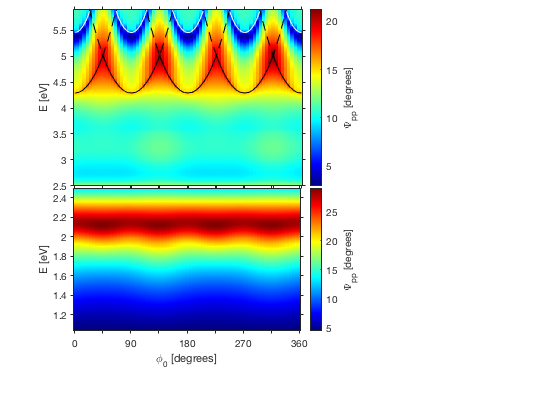
\includegraphics[width=0.99\linewidth, trim=1.1cm 1.8cm 6.7cm 0.3cm, clip]{figures/ch4/S6/contour/S6_Psipp.png}
        \caption{}
        \label{fig:S6_contour_peps}
    \end{subfigure}
    \caption{Contour plots of (a) $R_{pp}$ (b) $R_{ss}$ (c) $\text{Im}\langle\epsilon_{pp}\rangle$ and (d) $\Psi_{pp}$ as functions of photon energy $E$ and azimuthal angle $\psi_0$ for sample 6. Rayleigh lines corresponding to the 1st BZ are included as white and black lines for air and substrate, respectively. Extended Rayleigh lines are also included as dashed lines. Due to the strong LSPR around $2.1$ eV, separate colorbars are plotted for energies above and below $2.5$ eV.} %
    \label{fig:S6_contour_Rpp&Rss_peps&Psipp}
\end{figure}

Reflectance coefficients $R_{pp}$ and $R_{ss}$ as functions of photon energy and incident azimuthal angle can be found in figure \ref{fig:S6_contour_Rpp} and \ref{fig:S6_contour_Rss}, respectively. The LSPR can be seen at $2.1$ eV, fluctuating slightly. In order to better visualize the features weaker than the strong LSPR, a different colorbar is used for energies $E>2.5$ eV. The optical response for these energies are attributed to the Rayleigh anomalies related to grazing diffracted waves just at the onset of diffracted orders\cite{Brakstad:15}. The expression for the Rayleigh anomaly condition, equation (\ref{eq:RayleighLines}), is used to find for which wavelength and incidence azimuthal angle a particular diffraction order is triggered along the sample surface. These are superposed in figure \ref{fig:S6_contour_Rpp&Rss_peps&Psipp} and hereby referred to as \emph{Rayleigh lines}. The black lines correspond to the onset of the first diffraction mode in substrate (SiO$_2$) while the white lines similarly correspond to the first diffraction mode in the ambient (air). The dashed lines serves as \emph{extended} Rayleigh lines, which are defined as those lines calculated from equation (\ref{eq:RayleighLines}) for e.g. $45^\circ \leq \phi_0 \leq 90^\circ$ using $\mathbf{G}_\parallel^{\bar{1}0}$. In figures \ref{fig:S6_contour_peps} and \ref{fig:S6_contour_Psipp} the imaginary part of the pseudo-dielectric function $\text{Im}\langle\epsilon_{pp}\rangle$ and the ellipsometric angle $\Psi_{pp}$ are presented. Rayleigh lines for glass corresponding to 1st BZ are seen to follow peaks in $\Psi_{pp}$, while for air they follow dips. The same Rayleigh lines are observed at peaks in $R_{pp}$ at the M-point, i.e. $\phi_0=45^\circ$ in figure \ref{fig:S6_contour_Rpp}. In $R_{ss}$, the extended Rayleigh lines for glass are seen to act as boundaries of a region with medium-sized peaks.


Contour plots of the matrix elements of the normalized MM of sample 6 is presented in figure \ref{fig:S6_contour_MM}, where the photon energy $E$ and the azimuthal rotation angle $\phi_0$ represent the radius and the angle in each polar plot, respectively. One can observe that the MM is nearly block-diagonal, i.e. similar in shape as equation (\ref{eq:isotropicMM}) for non-depolarizing isotropic samples, for photon energies up till about $4$ eV. The LSPR is observed as a near-perfect circle around $2.1$ eV in all block diagonal elements. Rayleigh lines corresponding to the boundary of the 1st BZ in air (white lines) and substrate (black semi-square) are superposed in MM elements $m_{21}$ and $m_{33}$. In element $m_{24}$ the extended Rayleigh lines are additionally included. A slight polarization coupling is observed around the LSPR in the off-block-diagonal elements, while a stronger polarization conversion is clearly observed in the regions surrounding the Rayleigh lines of the same elements. The polarization coupling is more visible in the contour plots of $R_{sp}$, $R_{ps}$, $\Psi_{sp}$ and $\Psi_{ps}$ found in figure \ref{fig:S6_contour_Rsp&Rps_Psisp&Psips}. For convenience, figure \ref{fig:reciprocallattice} is repeated here in figure \ref{fig:S6_reciprocallattice_schematic}, showcasing how the azimuthal angle $\phi_0$ is defined as zero along the $\Gamma-X$-point of the reciprocal lattice.

The normalized MM of the experimental data can be found in figure \ref{fig:S6_contour_MM_exp}, to be readily compared with figure \ref{fig:S6_contour_MM}. In figure \ref{fig:S6_NCS} experimental data is compared to COMSOL data in terms of the MM elements $N=m_{12}$, $C=m_{33}$, and $S=m_{34}$ for three selected angles. Note that $N$ and $\Psi_{pp}$ have similar profiles. The COMSOL simulation is found to be in good compliance with the experimental data. It is interesting, however, to note an additional polarization coupling observed at around $3$ eV in elements $m_{31}$ and $m_{32}$ in figure \ref{fig:S6_contour_MM}, which is not observed in the experimental data.

%\clearpage
\begin{figure}[h]  %% radial MM
\begin{subfigure}{\textwidth}
    \centering
    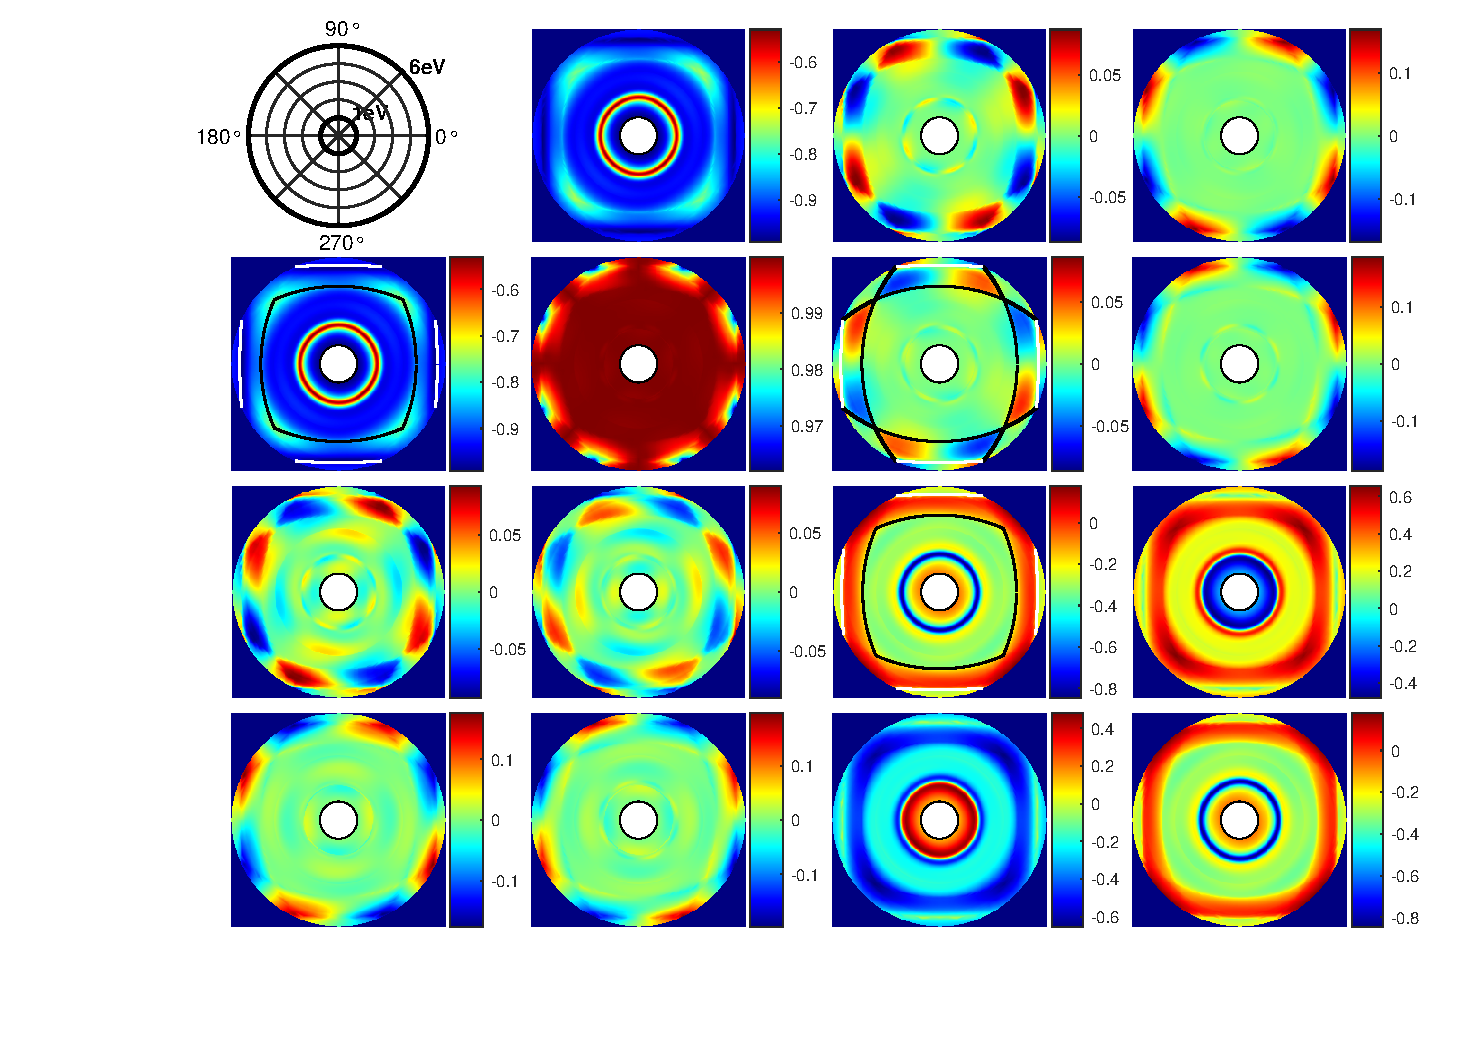
\includegraphics[width=\linewidth, trim=3cm 1.5cm 0.5cm 0cm, clip]{figures/ch4/S6/contour/Mueller_rot_S6_COMSOLSIM_55(2)(1).pdf}
    
\end{subfigure}

\begin{subfigure}{\textwidth}
\begin{subfigure}{0.5\textwidth}
        \flushright
        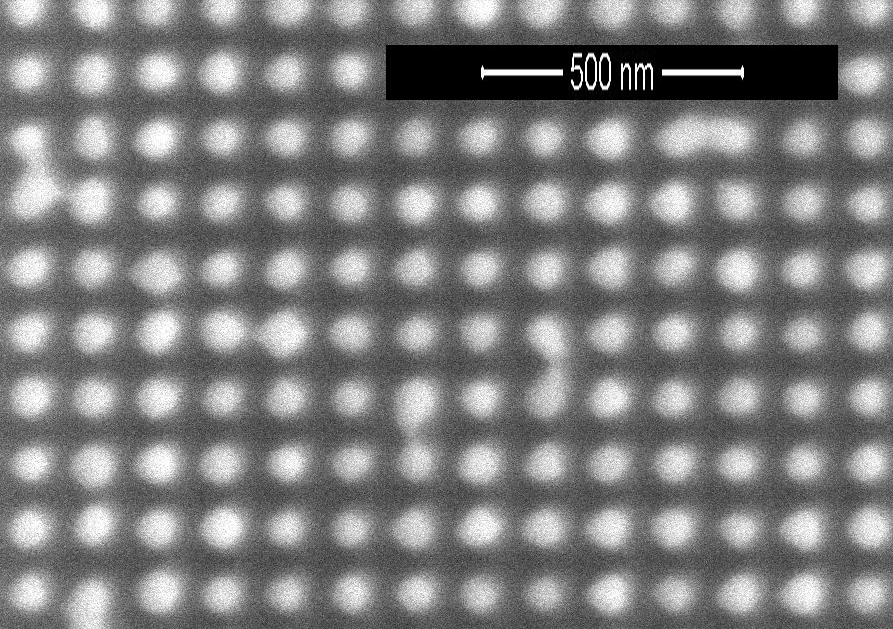
\includegraphics[width=0.5\linewidth]{figures/Ch3/S6_SEM(1).png} %0.4
    \end{subfigure}
    \begin{subfigure}{0.5\textwidth}
        \flushleft
        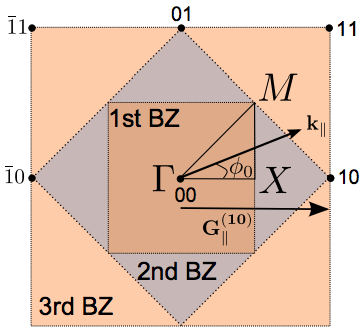
\includegraphics[width=0.4\linewidth]{figures/Ch2/ReciprocalLattice.png}    %0.33
    \end{subfigure}
    %\caption{}
    \label{fig:S6_reciprocallattice_schematic}
\end{subfigure}
    \caption{Contour plots of MM elements for sample 6 as simulated in COMSOL, where photon energy $E$ and azimuthal angle $\phi_0$ of the incident light corresponds to the radius and angle in each polar plot, respectively. The inner circle of the plots denote the lower limit photon energy of $1.03$ eV, while the outer circle corresponds to $5.9$ eV. In elements $m_{21}$ and $m_{33}$ the Rayleigh lines for BZ-1 in glass (black line) and air (white line) are shown, while element $m_{23}$ in addition includes the extended Rayleigh line for BZ-1 in glass. A SEM image of sample 6 next to a schematic of a square reciprocal lattice defining incidence angle $\phi_0$ has been included below the MM.}
    \label{fig:S6_contour_MM} 
\end{figure}
\begin{figure}[h]
    
\end{figure}
\begin{figure}[h]
    \centering
    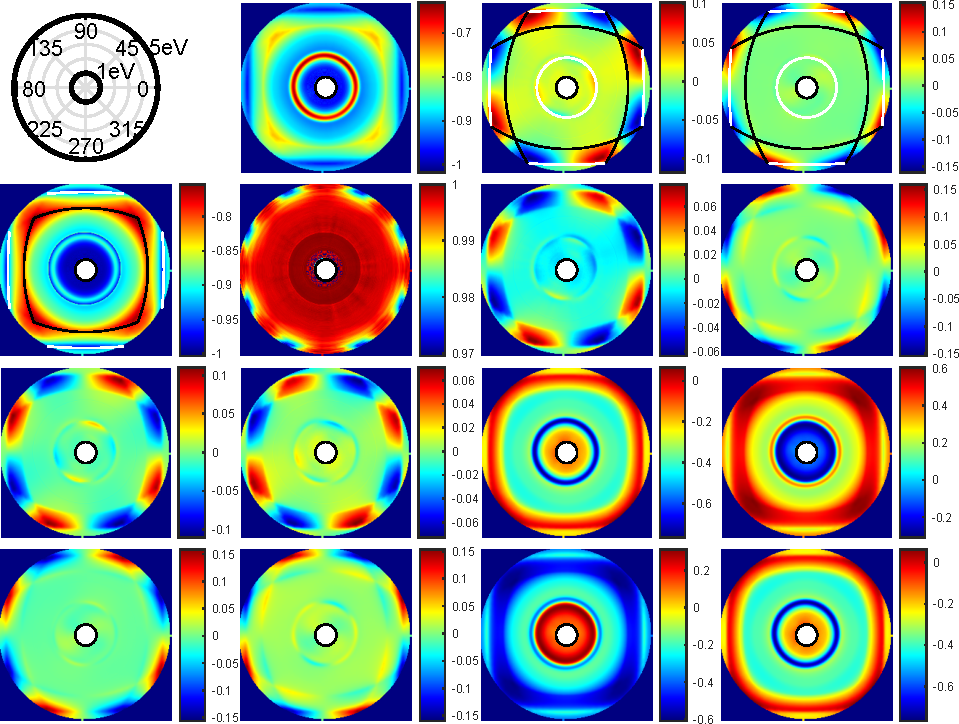
\includegraphics[width=\linewidth]{figures/ch4/S6/exp/Muller_rot_S6_55.pdf}
    \caption{The experimental MM of sample 6, where the energy is plotted radially and the rotation angle is the azimuthal angle $\phi_0$, and the polar AOI is $\theta_0=55^\circ$. Inner circle corresponds to $0.73$ eV while outer circle corresopnd to $5.9$ eV. Rayleigh lines are superposed in elements $m_{21}$, $m_{13}$ and $m_{14}$. A scaling has been applied to $m_{21}$ for improved visibility \text{\color{red}MK:vet du hvilken scaling?}. Data from \cite{brakstad_thesis}.}
    \label{fig:S6_contour_MM_exp}
\end{figure}
\begin{figure}[h]
   \begin{subfigure}{0.32\linewidth}
        \centering
        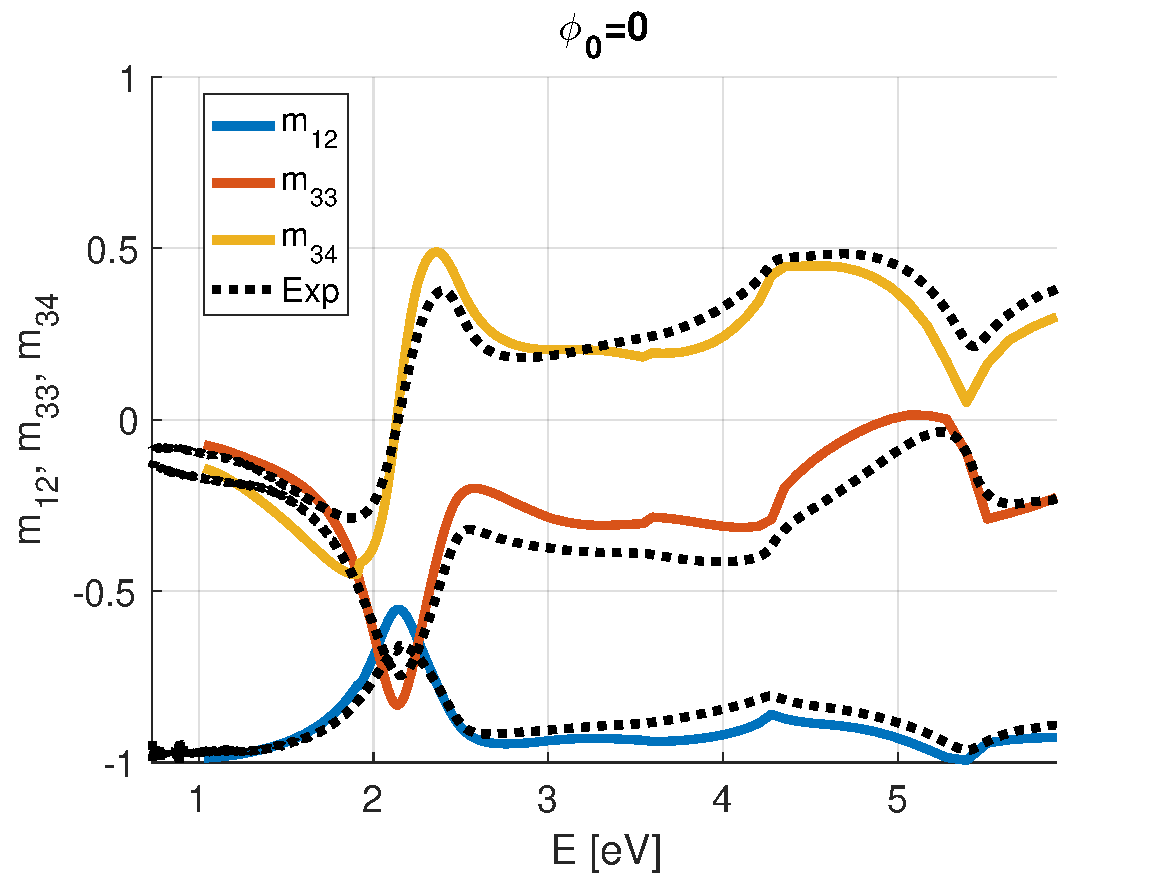
\includegraphics[width=\linewidth, trim= 0cm 0cm 2cm 0cm, clip]{figures/ch4/S6/NCS/S6_NCS_phi0.pdf}
   \end{subfigure}
   \begin{subfigure}{0.32\linewidth}
        \centering
        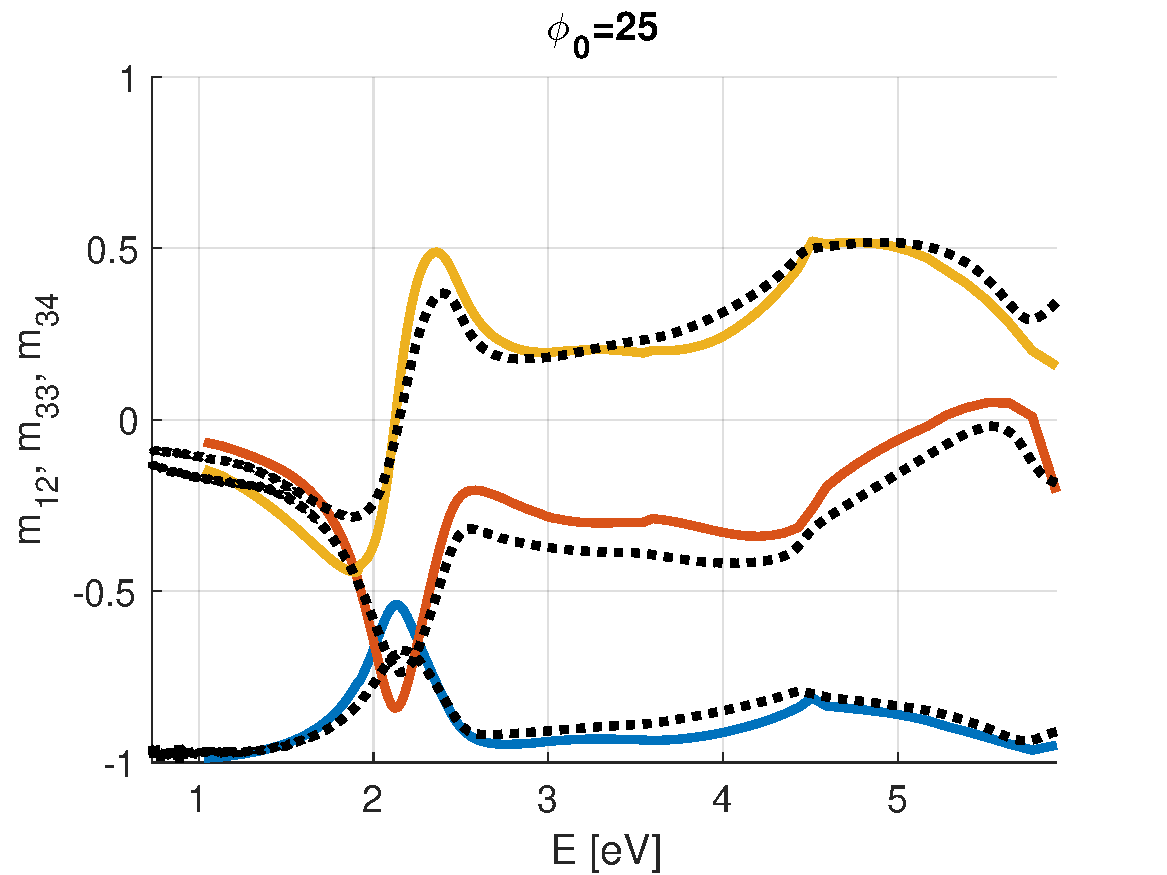
\includegraphics[width=\linewidth, trim= 0cm 0cm 2cm 0cm, clip]{figures/ch4/S6/NCS/S6_NCS_phi25.pdf}
   \end{subfigure}
   \begin{subfigure}{0.32\linewidth}
        \centering
        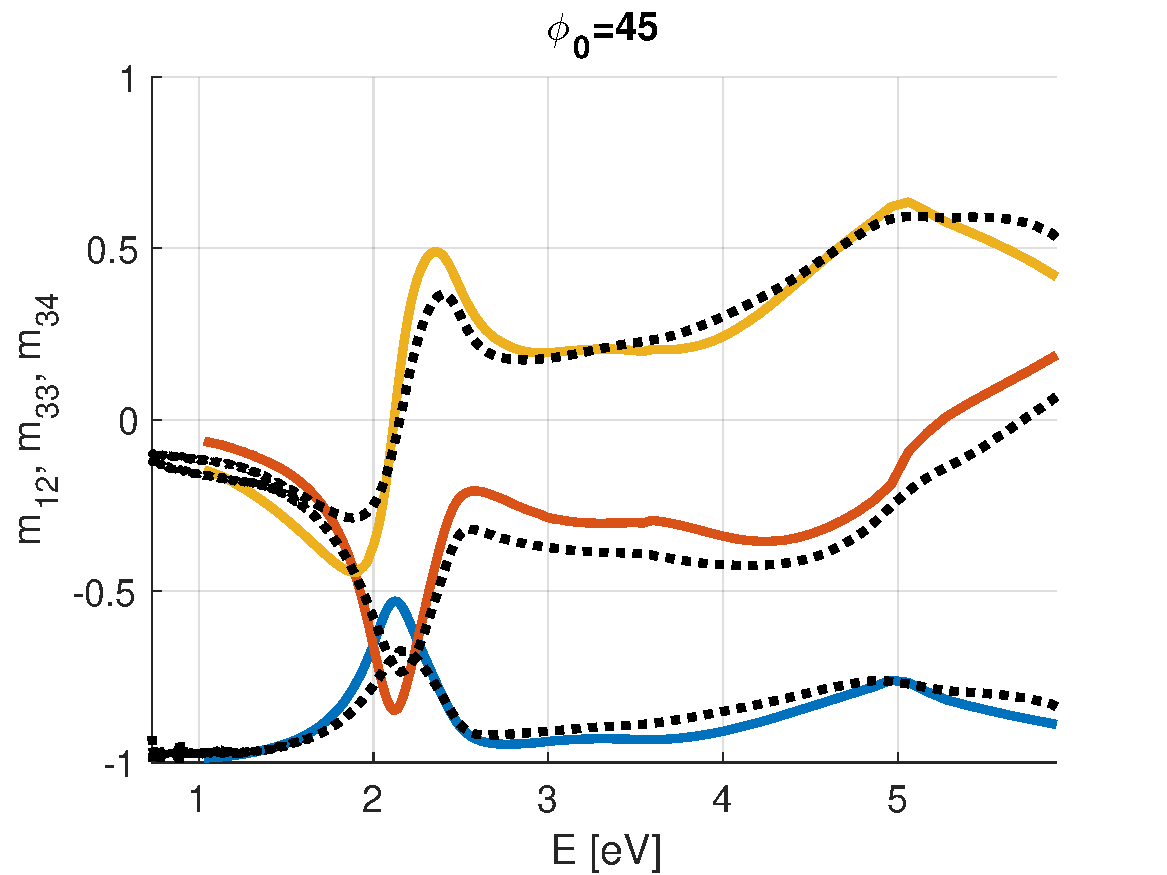
\includegraphics[width=\linewidth, trim= 0cm 0cm 2cm 0cm, clip]{figures/ch4/S6/NCS/S6_NCS_phi45.pdf}
   \end{subfigure}
   \caption{Sample 6 comparison between simulation (solid colored lines) and experimental data (black dashed lines) of the MM elements $m_{12}$,$m_{33}$ and $m_{34}$.}
   \label{fig:S6_NCS}
\end{figure}
\begin{figure}[h]  %% Psi_ps & Psi_sp contour E and phi
    \begin{subfigure}{0.5\textwidth}
        \centering
        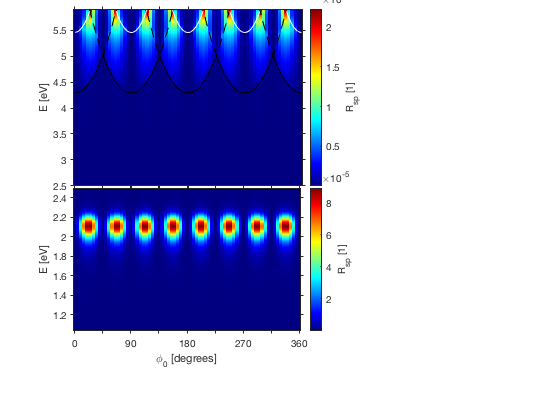
\includegraphics[width=\linewidth, trim=1.1cm  1.8cm 6.7cm 0cm, clip]{figures/ch4/S6/contour/S6_Rsp.png}
    \end{subfigure}
    \begin{subfigure}{0.5\textwidth}
        \centering
        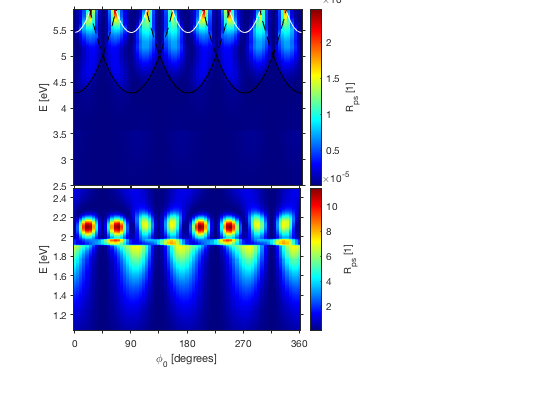
\includegraphics[width=\linewidth, trim=1.1cm  1.8cm 6.7cm 0cm, clip]{figures/ch4/S6/contour/S6_Rps.png}
    \end{subfigure}
    
    \begin{subfigure}{0.5\textwidth}
        \centering
        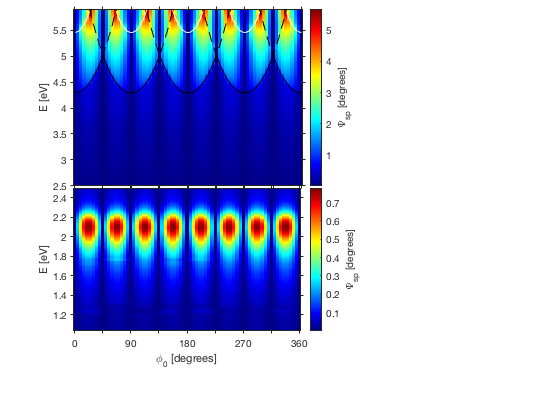
\includegraphics[width=\linewidth, trim=1.1cm 1.8cm 6.7cm 0.3cm, clip]{figures/ch4/S6/contour/S6_Psisp.png}
        \caption{}
    \end{subfigure}
    \begin{subfigure}{0.5\textwidth}
        \centering
        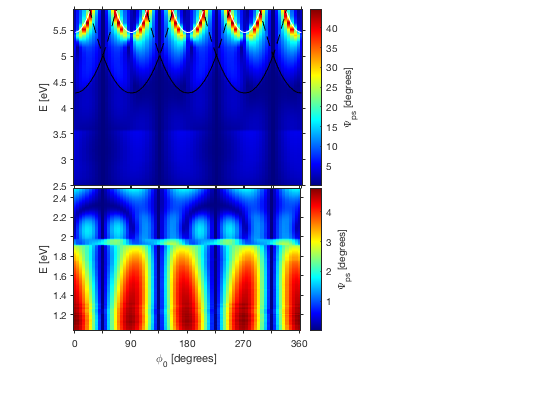
\includegraphics[width=\linewidth, trim=1.1cm 1.8cm 6.7cm 0.3cm, clip]{figures/ch4/S6/contour/S6_Psips.png}
        \caption{}
    \end{subfigure}
    \caption{Contour plots of (a) $R_{sp}$ (b) $R_{ps}$ (c) $\Psi_{sp}$ and (d) $\Psi_{ps}$ for sample 6. For reasons of clarity, separate colorbars are implemented for energies $E>2.5$ eV. \color{red}fix x$10^{-3}$}
    \label{fig:S6_contour_Rsp&Rps_Psisp&Psips}
\end{figure}




\begin{figure}[h!]
    \begin{subfigure}{0.5\textwidth}
        \centering
        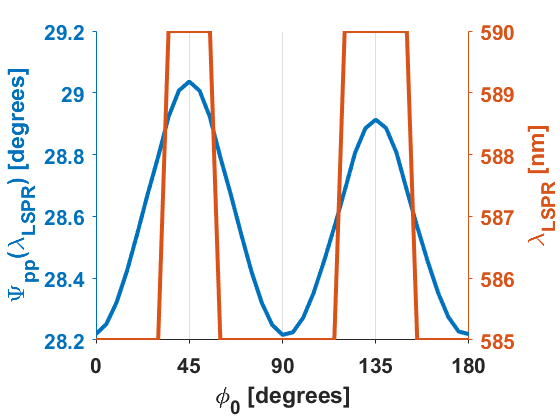
\includegraphics[width=0.8\linewidth, trim=0cm  0cm 0cm 0cm, clip]{figures/ch4/S6/S6_Psi_pp@LSPR.png}
        \caption{}
        \label{fig:S6_LSPRvsphi_Psipp}
    \end{subfigure}
    \begin{subfigure}{0.5\textwidth}
        \centering
        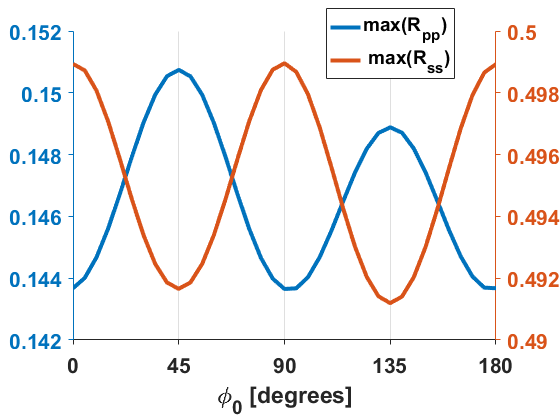
\includegraphics[width=0.8\linewidth, trim=0cm  0cm 0cm 0cm, clip]{figures/ch4/S6/S6_Rpp_Rss@LSPR.png}
        \caption{}
        \label{fig:S6_LSPRvsphi_RppRss}
    \end{subfigure}
    \caption{(a) Peak values of $\Psi_{pp}$ for sample 6 at LSPR wavelengths $\lambda_{\text{LSPR}}$, plotted together with the wavelength at which the plasmon resonance peaks for a given $\phi_0$; (b) Azimuthal angle dependency of reflectances for p-polarized and s-polarized light $R_{pp}$ and $R_{ss}$, respectively, at plasmon resonance wavelengths shown in (a).}
    \label{fig:S6_LSPRvsphi}
\end{figure}
\begin{figure}[h!]  %% Resistive Heat Loss
    \begin{subfigure}{\textwidth}
        \centering
        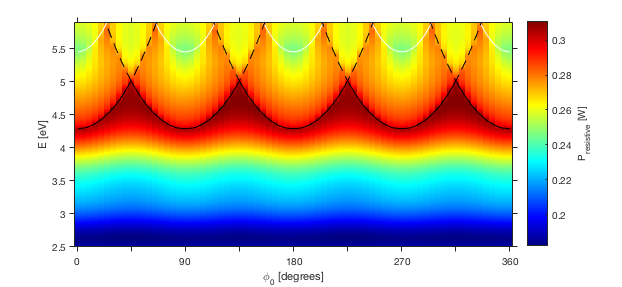
\includegraphics[width=0.8\linewidth, trim=0cm 0cm 1cm 0.5cm, clip]{figures/ch4/S6/contour/S6_HeatLoss_contour(1).png}
    \end{subfigure}
    
    \begin{subfigure}{\textwidth}
        \centering
        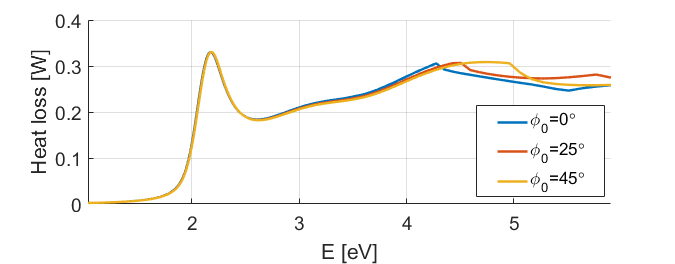
\includegraphics[width=0.6\linewidth, trim=0cm 0cm 0cm 0cm, clip]{figures/ch4/S6/contour/S6_HeatLoss_phi=0,25,45.png}
    \end{subfigure}
    
    \caption{Top: Contour plot of resistive heat loss over the volume of the gold particles in sample 6, with respect to photon energy and azimuthal angle of the incident light. Rayleigh lines corresponding to the 1st BZ in air (white lines) and glass substrate (black lines) have been superimposed. Bottom: Same plot but the full energy spectrum for a few chosen values of $\phi_0$, illustrating isotropic behaviour below 2.5 eV.}
    \label{fig:S6_heatloss}
\end{figure}
In previous figures there can be observed a small fluctuation of the LSPR. In figure \ref{fig:S6_LSPRvsphi_Psipp} the peak value of $\Psi_{pp}$ at the LSPR is plotted as a function of the incident azimuthal angle, together with the wavelength $\lambda_{\text{LSPR}}$ at which $\Psi_{pp}$ is at maximum. Obviously, using a smaller stepsize for wavelength would smoothen out the latter curve. The peak resonance of the LSPR exhibit a small dependency on azimuthal angle of incidence. Given the uniformity of sample 6 ($R_{x}=R_{y}$ and $a_x=a_y$), one might expect a $45^\circ$ symmetry. However, there is clearly anomalies to this at $45^\circ$ and $135^\circ$. \text{\color{red}Why?}

Figure \ref{fig:S6_heatloss} shows a contour plot of heat dissipation $P_{\text{resistive}}$ integrated over Au particle volume as a function of the energy $E$ and azimuthal angle $\phi_0$ of the incident light. For energies below $2.5$ eV the heat loss is uniform for all azimuthal angles. Observe that peaks in $P_{\text{resistive}}$ follow Rayleigh lines of the substrate, while Rayleigh lines of the ambient air are recognized by dips in $P_{\text{resistive}}$.

Figure \ref{fig:S6_normE_isosurface_LSPR} visualize the electric field norm $E_\text{norm}$ in the 3D space surrounding the Au particle and mound area. Red isosurface correspond to the strongest field (barely visible) while dark blue is weaker. The LSPR is seen to be strongly concentrated along the bottom edge of the gold particle.
\begin{figure}[h]
    \begin{subfigure}{0.32\textwidth}
        \centering
        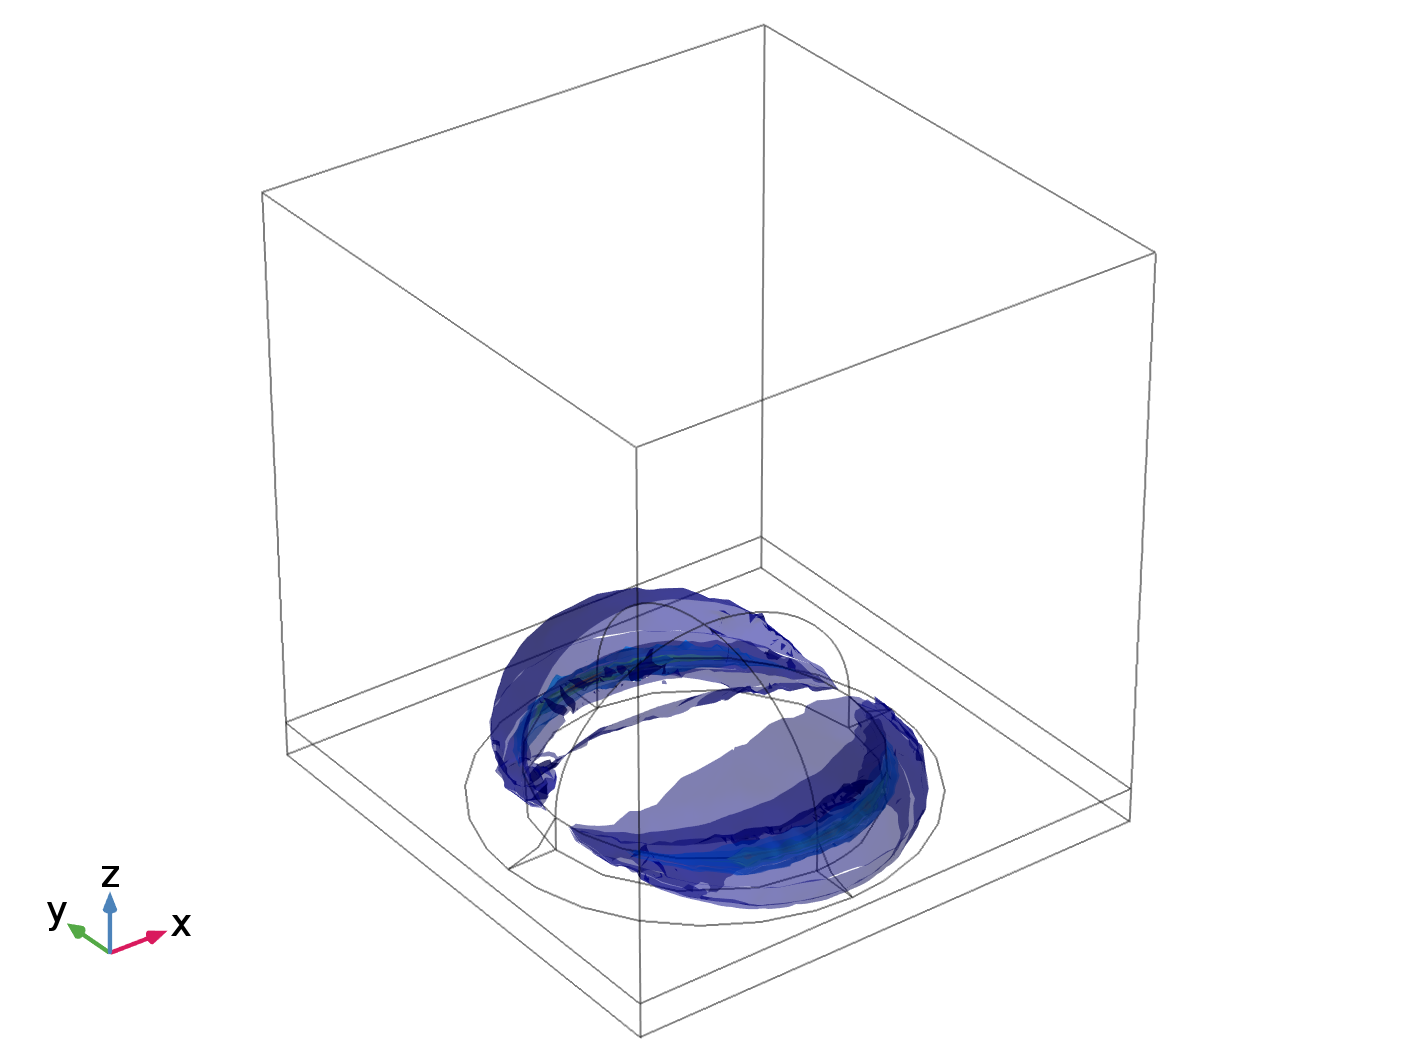
\includegraphics[width=\linewidth, trim=0.4cm 0 1.5cm 0, clip]{figures/ch4/S6/normE/Sample6_nomE_wl585_phi0_TE.png}
        \caption{}
    \end{subfigure}
    \begin{subfigure}{0.33\textwidth}
        \centering
        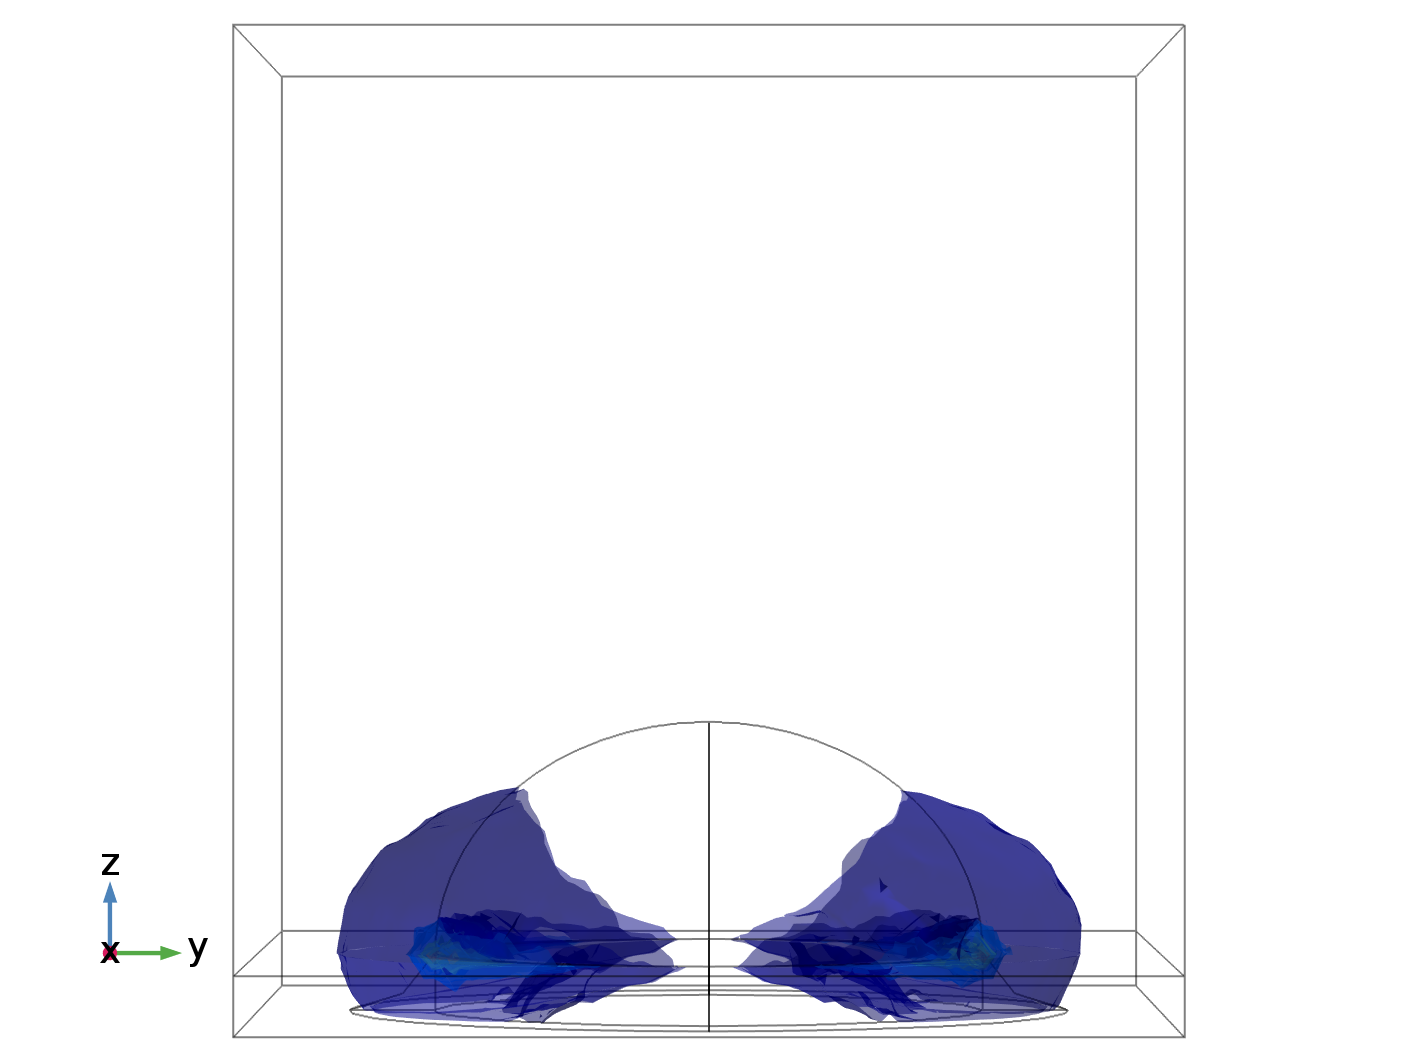
\includegraphics[width=\linewidth, trim=0.6cm 0 1.6cm 0, clip]{figures/ch4/S6/normE/Sample6_nomE_wl585_phi0_TE_xtowardsviewer.png}
        \caption{}
    \end{subfigure}
    \begin{subfigure}{0.33\textwidth}
        \centering
        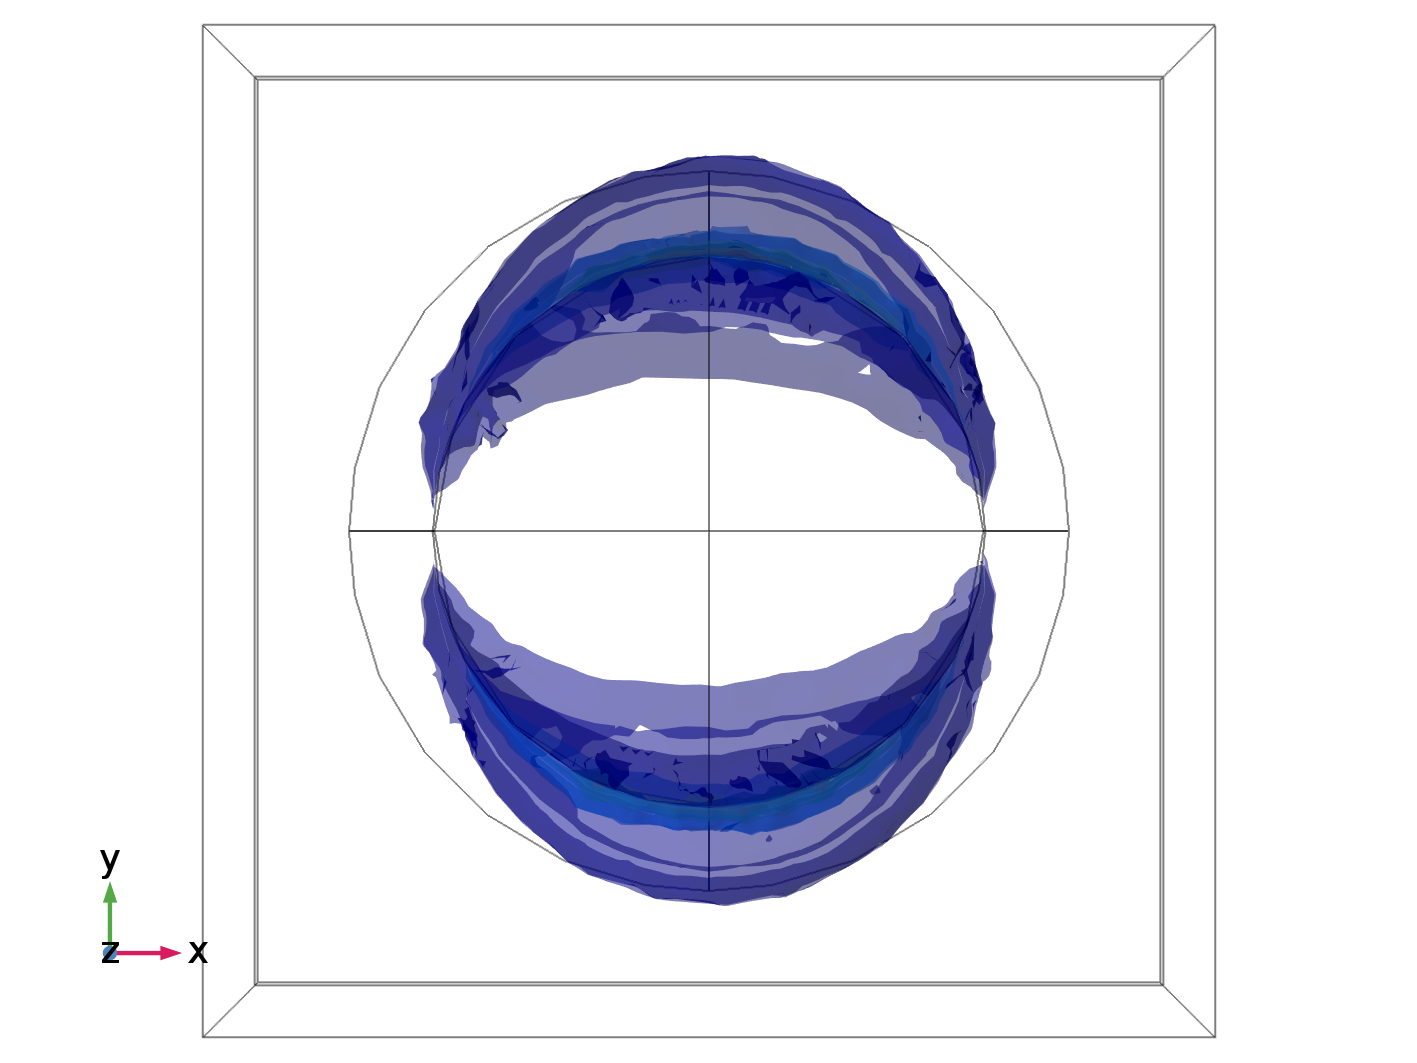
\includegraphics[width=\linewidth, trim=0.6cm 0 1.6cm 0, clip]{figures/ch4/S6/normE/Sample6_nomE_wl585_phi0_TE_ztowardsviewer.png}
        \caption{}
    \end{subfigure}
    \caption{The electric field norm $E_\text{norm}$ plotted for five layers of isosurface when incident wave is TE polarized at wavelength $\lambda_{\text{LSPR}}=585$ nm and azimuthal angle $\phi_0=0^\circ$, i.e. propagating along $\hat{x}$-direction at polar incidence $\theta_0=55^\circ$. (a) General view (b) $\hat{x}$ is pointing out of paper (b) $\hat{z}$ is pointing out of paper.}
    \label{fig:S6_normE_isosurface_LSPR}
\end{figure}
\begin{figure}[h]
    \begin{subfigure}{0.32\textwidth}
        \centering
        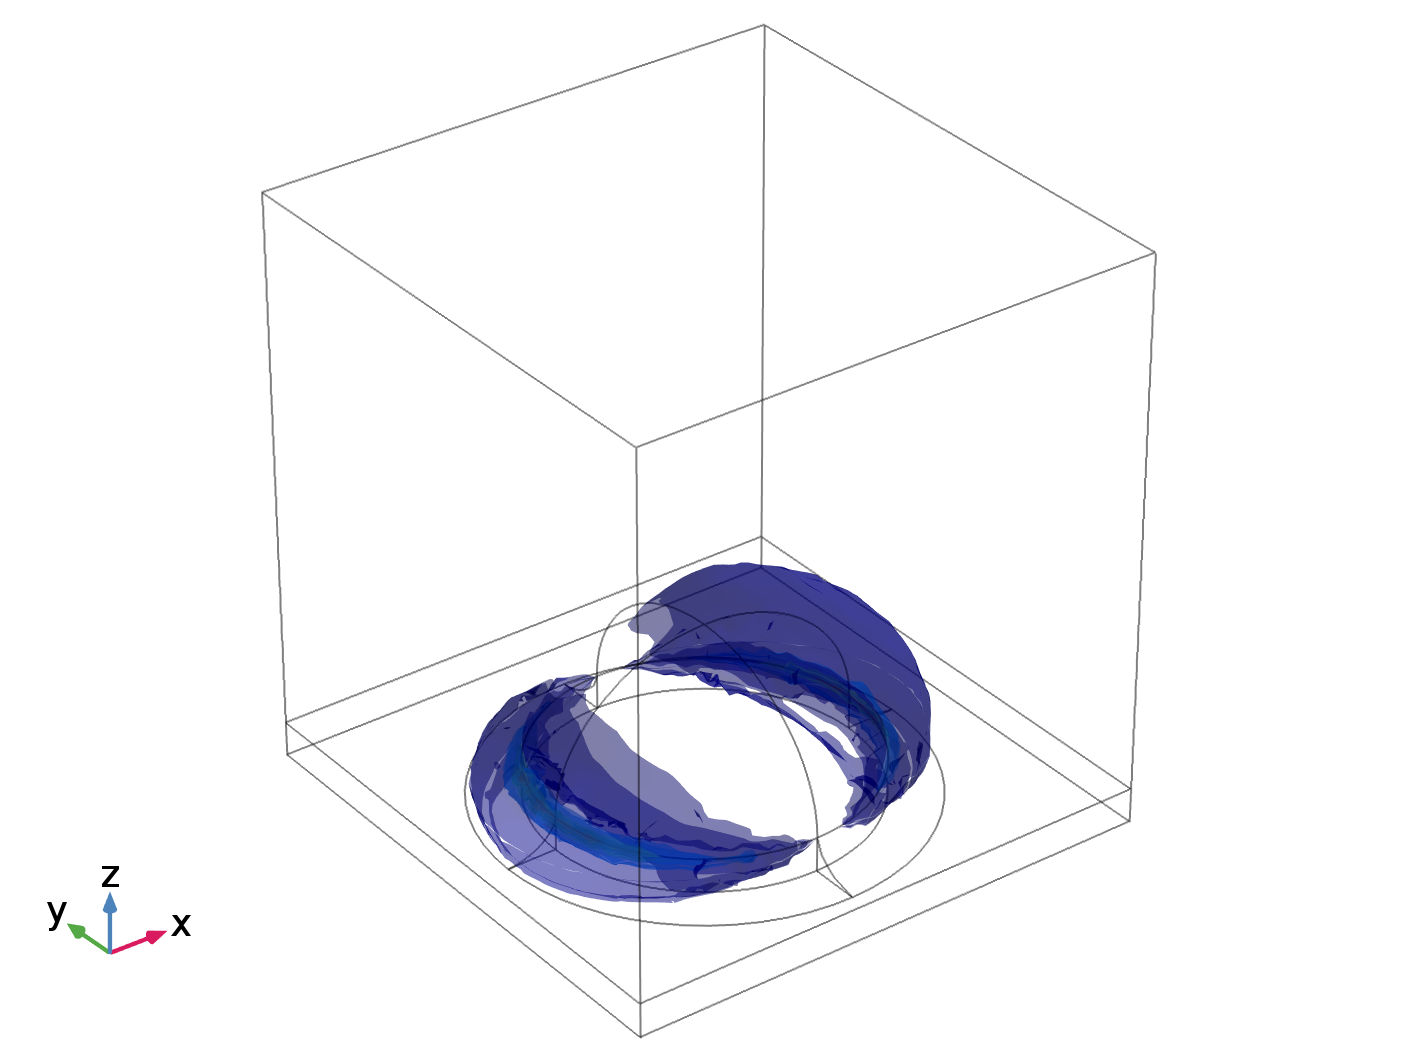
\includegraphics[width=\linewidth, trim=0.4cm 0 1.5cm 0, clip]{figures/ch4/S6/normE/Sample6_nomE_wl585_phi0_TM.png}
        \caption{}
    \end{subfigure}
    \begin{subfigure}{0.33\textwidth}
        \centering
        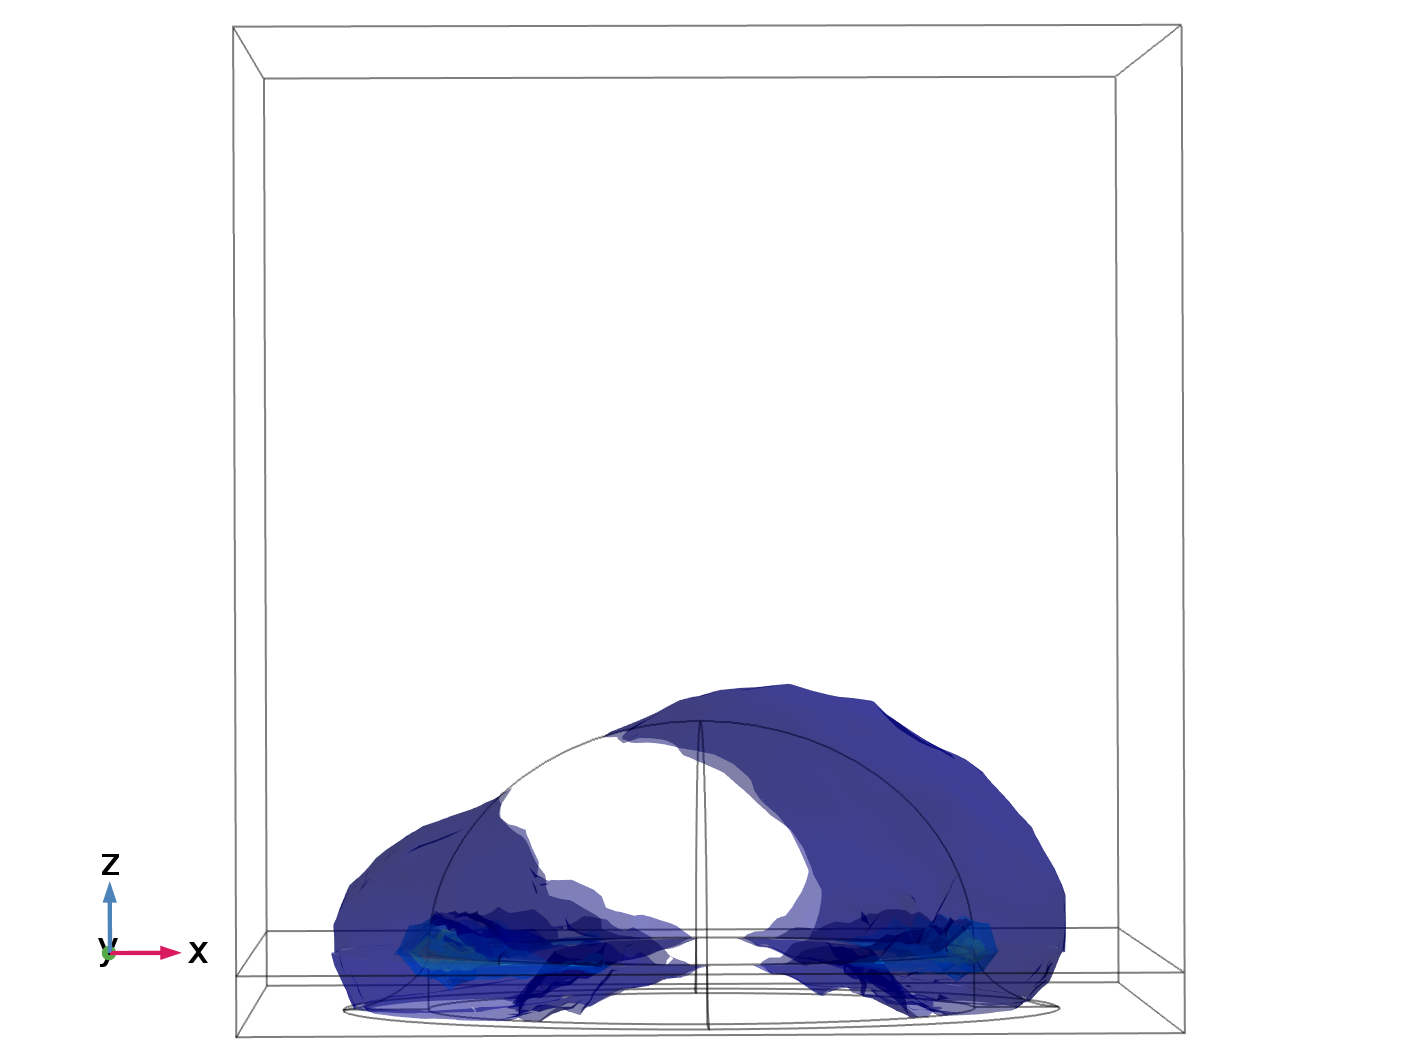
\includegraphics[width=\linewidth, trim=0.6cm 0 1.6cm 0, clip]{figures/ch4/S6/normE/Sample6_nomE_wl585_phi0_TM_yawayfromviewer.png}
        \caption{}
    \end{subfigure}
    \begin{subfigure}{0.33\textwidth}
        \centering
        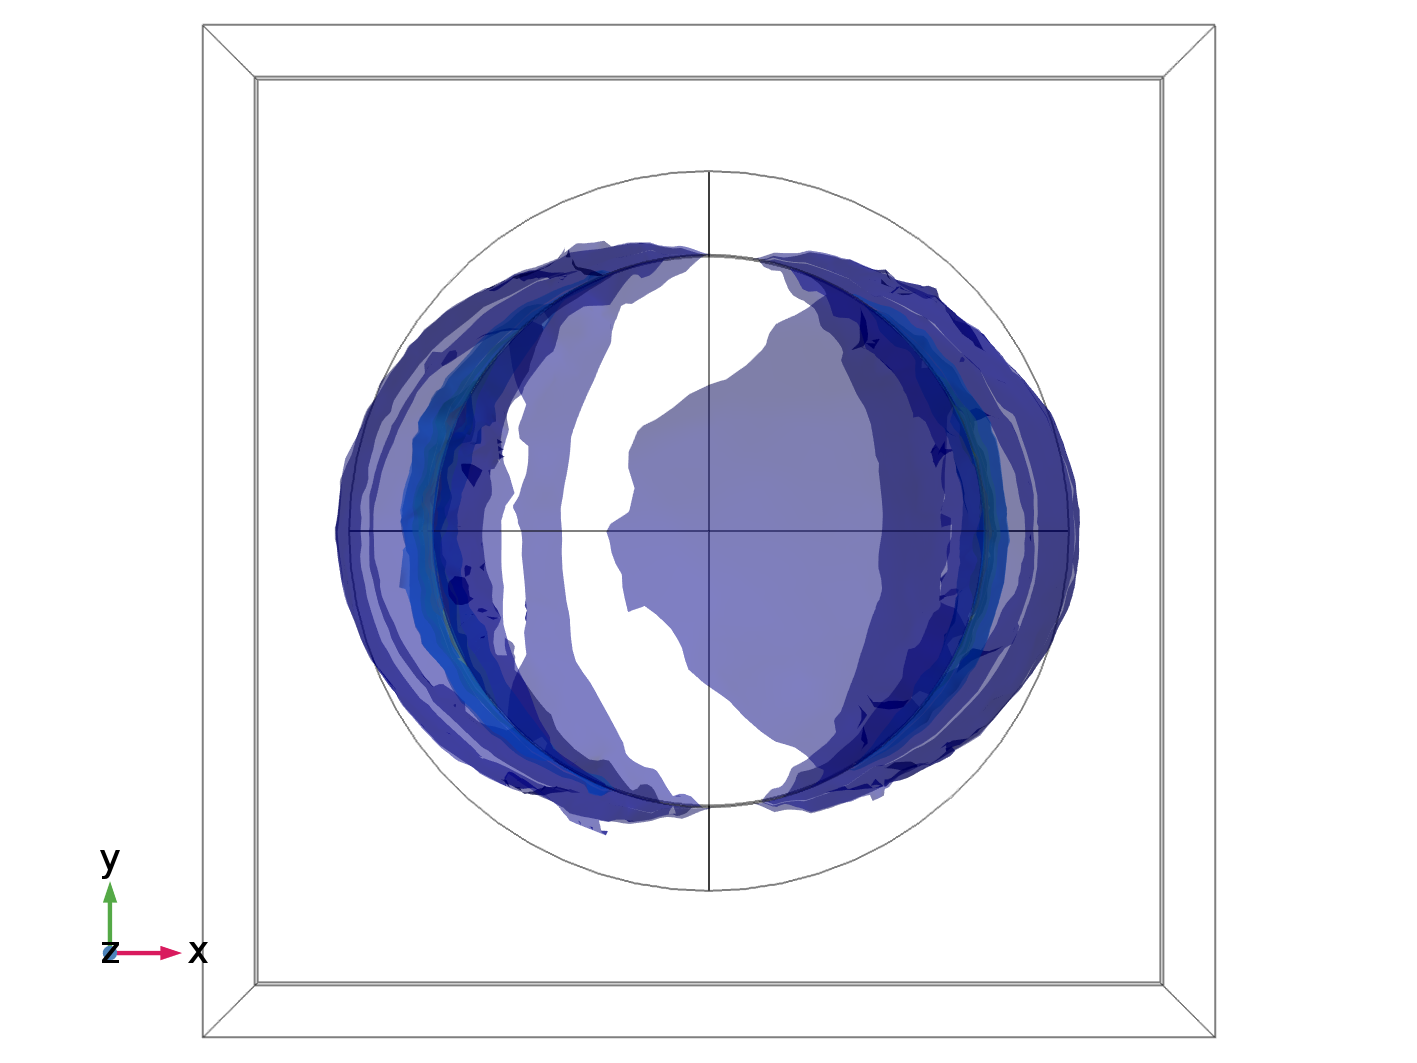
\includegraphics[width=\linewidth, trim=0.6cm 0 1.6cm 0, clip]{figures/ch4/S6/normE/Sample6_nomE_wl585_phi0_TM_ztowardsviewer.png}
        \caption{}
    \end{subfigure}
    \caption{The electric field norm $E_\text{norm}$ plotted for five layers of isosurface when incident wave is TM polarized at wavelength $\lambda_{\text{LSPR}}=585$ nm and azimuthal angle $\phi_0=0^\circ$, i.e. propagating along $\hat{x}$-direction at polar incidence $\theta_0=55^\circ$. (a) General view (b) $\hat{y}$ is pointing into the paper (b) $\hat{z}$ is pointing out of paper.}
    \label{fig:S6_normE_isosurface_LSPR}
\end{figure}



%%%%%%%%%%%%%%%%%%%%%%%%%%%%%
%\subsection{Effects of the mound \color{red}fjern?}

%\begin{itemize}
    %\item Shape of mound more or less arbitrarily chosen as a smooth parabolic(?) as shown in figure [ref til fig av mound/Au sample6)]. 
%    \item Hvis tid: sammenlikn med mound som trekant (i tverrsnitt)
%\end{itemize}

\clearpage
%%%%%%%%%%%%%%% NEW SECTION %%%%%%%%%%%%%%%
\section{Sample 5A}
Due to the symmetry of the sample, it was deemed sufficient to simulate only for the first half of the azimuthal angles, then mirroring the results to gain the full rotational optical response. The total wall time, including both TE and TM simulations, each running for wavelengths $\lambda=210-1600$ nm with stepsize $\Delta\lambda=5$ nm and an auxiliary sweep of incident azimuthal angles $\phi_0=0^\circ-180^\circ$ with stepsize $\Delta\lambda=5^\circ$, was 38 hours and 50 minutes. In practice the actual simulation run-time is halved as both TE and TM simulations were running simultaneously. The approximate CPU time is 9 days and 17 hours when assuming the workload was at all times evenly distributed among the six CPU cores. Each of the two simulations used at most around $9.5$ GB RAM during the calculation, and spent 23 minutes solving $\lambda=210$ nm for all the incident angles whereas $\lambda=1600$ nm for all angles was completed in 1 min 40 seconds.

The reflectances from both TE and TM simulations with respect to the energy and azimuthal angle of the incident beam can be found in figures \ref{fig:S5A_contour_Rpp}-b. One immediately observes patterns forming in the higher energy region as well as a strong LSPR resonance around $2$ eV. The LSPR is seen to fluctuate with respect to the incident angle, which is further investigated in figure \ref{fig:S5A_LSPRvsphi}. In figure \ref{fig:S5A_LSPRvsphi_Psipp}, where the resonance is represented by $\Psi_{pp}$, we see that the wavelength at which the LSPR is located $\lambda_{\text{LSPR}}$ is also shifted as the resonance fluctuates. Here we are reminded that the jagged lines are due to the relatively large stepsize of wavelength when scrutinizing a narrow region. On average, the LSPR is located at $\lambda_{\text{LSPR}}=625$ nm. Compared to the average LSPR position of the experimental sample, $\lambda_{\text{LSPR}}^\text{(exp)}=608$ nm, it might suggest that the sample parameters used in COMSOL are not entirely accurate. It is clear from these figures that sample 5A does not hold a perfect 45 degree symmetry, or even a 90 degree symmetry. Why this is, will be discussed in section \ref{sec:results_S5A_comparisons}.

Ellipsometric angle $\Psi_{pp}$ and the imaginary part of the pseudo dielectric function, $\text{Im}\langle\epsilon\rangle_{pp}$, are presented in figures \ref{fig:S5A_contour_Psipp}-d. Here, Rayleigh lines have been superposed revealing an optical response highly dependent on the diffracted modes along the surface. The very same Rayleigh lines can be observed in the reflectances in figures \ref{fig:S5A_contour_Rpp}-b without the aid of drawn lines. The Rayleigh lines correspond to 1st and 2nd BZ in air (white lines) and substrate (black lines), as well as the 3rd BZ in substrate (top black solid line). These lines are also overlaid in the contour plots of $\Psi_{sp}$ and $\Psi_{ps}$ in figure \ref{fig:S5A_contour_Psips&Psisp}, and in the normalized MM in figure \ref{fig:S5A_contour_MM}. 

The normalized MM of the experimental data can be found in in figure \ref{fig:S5A_contour_MM_exp}, and comparisons between experimental and COMSOL data of MM elements $m_{12}$, $m_{33}$ and $m_{34}$ at three specific azimuthal angles are found in figure \ref{fig:S5A_NCS}. In figures \ref{fig:S5A_stacked_PsippImeps} and \ref{fig:S5A_stacked_PsippImeps_exp}, $\Psi_{pp}$ and $\text{Im}\langle\epsilon\rangle_{pp}$ for angles $\phi_0=0^\circ-45^\circ$ are stacked on top of each other for COMSOL and experimental data, respectively. Figures \ref{fig:S5A_contour_MM}-\ref{fig:S5A_stacked_PsippImeps_exp} indicate a good agreement between simulated and experimental data. Note, however, that the off-block-diagonal elements have overall larger values in the simulated MM compared to the experimental MM, which suggest a stronger structure-induced anisotropy in the COMSOL model. This implies that the modeled dielectric mound is not quite true to its experimental counterpart, differing in shape or size or both, in which case would suggest that the estimated height profile is not as accurate as we thought. Figure \ref{fig:S5A_sumNCSsquared} plots equation (\ref{eq:sumNCSsquared=1}) for all energies and incident angles, indicating that the block-diagonal MM approach of equation (\ref{eq:isotropicMM}) can safely be assumed only at angles $\phi_0=0^\circ, 90^\circ$. \text{\color{red}usikker. hvor nærme $1$ burde man være?}

The main features of the optical response for photon energies above the LSPR can be described by estimating the Rayleigh line. Boundaries of 1st and 2nd BZ in air are clearly visible in the block-diagonal elements of the MM contour plot. For example, in the $m_{12}=m_{21}$ elements they are seen as sharp dips. Seeing as the MM to a certain extent follows the block-diagonal form of equation (\ref{eq:isotropicMM}), one can assume to observe a similar dip in $\Psi_{pp}$, as is shown in figure \ref{fig:S5A_stacked_PsippImeps}. The strong dips for BZ-1 in air also indicate that mainly p-polarized light is coupled into the grazing diffracted mode, as the reflected light contains a reduced amount of p-polarized light at this Rayleigh line. In contrast, the peaks at BZ-1 in the SiO$_2$ substrate suggests an enhanced reflection of p-reflectance (or reduced s-reflectance) of the reflected beam at the Rayleigh line condition.

%    \begin{itemize}
%       \item These dips are observed to follow the boundaries of the 1st and 2nd BZ with $n_i=1$ using equation (\ref{eq:RayleighLines}), i.e. diffracted beams in air directed along the substrate surface. Seeing as the MM (FIG radialMM REF) to a certain extent follows the block-diagonal form of equation (), one can assume to observe a similar dip in $\Psi_{pp}$, as is shown in figure (Fig5frompaper REF). The strong dips for BZ-1 [referring to Fig5frompaper] in air also indicate that mainly p-polarized light is coupled into the grazing diffracted mode, as the reflected light contains a reduced amount of p-polarized light at this Rayleigh line. In contrast, the peaks at BZ-1 in the SiO$_2$ substrate suggests an enhanced reflection of p-reflectance (or reduced s-reflectance) of the reflected beam at the Rayleigh line condition.
%    \end{itemize}
Due to the transparency of the substrate, grazing diffracted beams inside the glass substrate are also observed. Enhanced peaks of 1st BZ of SiO2 substrate at the $M$ point, i.e. $\phi_0=45^\circ$, for energies around $E_{BZ-1}^{sub}=3.1$ eV. The same peak in the experimental data is found at $3.08$ eV\cite{Brakstad:15}. A weaker, but broader peak is visible at the $X$ point for the glass Rayleigh line at $E_{BZ-2}^{\text{SiO}_2}=4.28$ eV, or at $4.15$ eV in the experimental data. These peaks are visible in figures \ref{fig:S5A_stacked_PsippImeps} and \ref{fig:S5A_stacked_PsippImeps_exp}, but also in the contour plots in figures \ref{fig:S5A_contour_Rpp&Rss_Psipp&Imeps} and \ref{fig:S5A_contour_MM} when inspecting the 1st and 2nd Rayleigh lines for the substrate at azimuthal angles $\phi_0=45^\circ, 0^\circ$, respectively.

\begin{figure}
    \begin{subfigure}{0.5\textwidth}
        \centering
        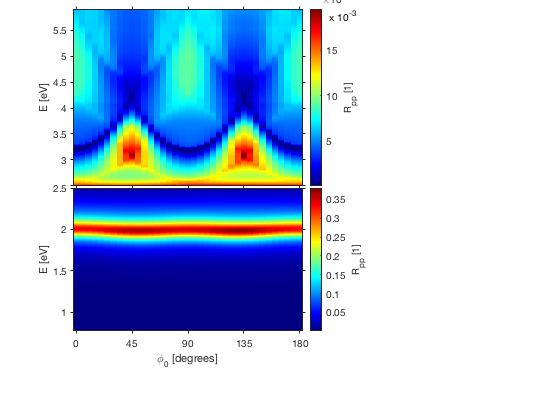
\includegraphics[width=\linewidth, trim=1.1cm 1.8cm 6.7cm 0.3cm, clip]{figures/ch4/S5A/contour/S5A_Rpp.png}
        \caption{}
        \label{fig:S5A_contour_Rpp}
    \end{subfigure}
    \begin{subfigure}{0.5\textwidth}
        \centering
        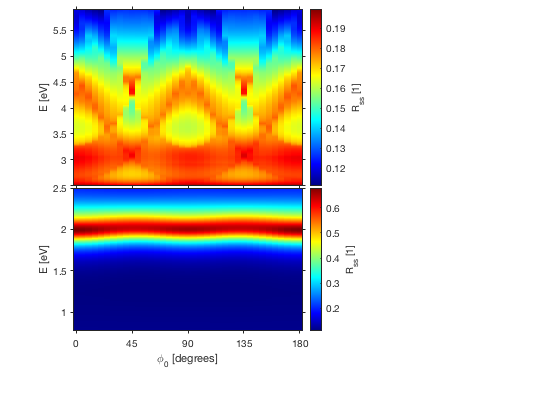
\includegraphics[width=\linewidth, trim=1.1cm 1.8cm 6.7cm 0.3cm, clip]{figures/ch4/S5A/contour/S5A_Rss.png}
        \caption{}
        \label{fig:S5A_contour_Rss}
    \end{subfigure}
    
    \begin{subfigure}{0.5\textwidth}
        \centering
        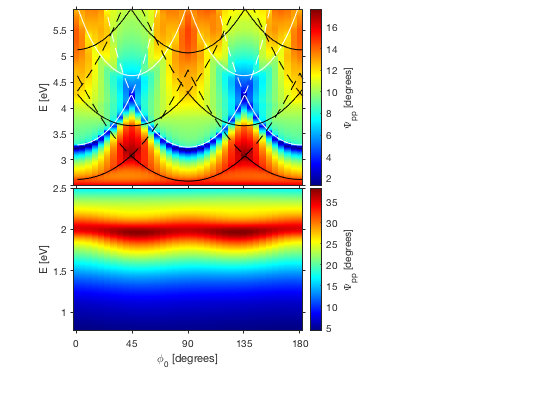
\includegraphics[width=\linewidth, trim=1.1cm 1.8cm 6.7cm 0.3cm,, clip]{figures/ch4/S5A/contour/S5A_Psipp.png}
        \caption{}
        \label{fig:S5A_contour_Psipp}
    \end{subfigure}
    \begin{subfigure}{0.5\textwidth}
        \centering
        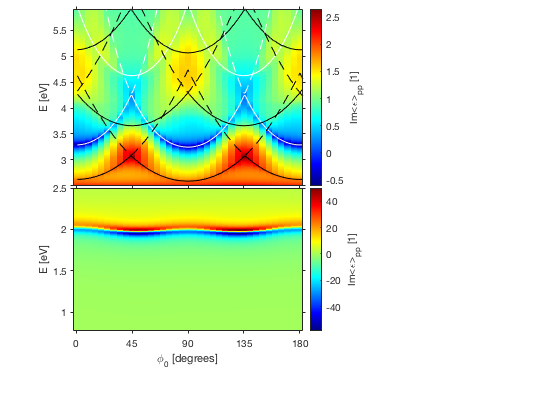
\includegraphics[width=\linewidth, trim=1.1cm 1.8cm 6.7cm 0.3cm,, clip]{figures/ch4/S5A/contour/S5A_peps.png}
        \caption{}
        \label{fig:S5A_contour_Imeps}
    \end{subfigure}
    \caption{Simulation results of sample 5A represented by contour plots of (a) $R_{pp}$ (b) $R_{ss}$ (c) $\Psi_{pp}$ and (d) $\text{Im}\langle\epsilon\rangle_{pp}$, as functions of energy $E$ and azimuthal angle $\phi_0$ of the incident beam. Due to the strong LSP resonance around $2$ eV, all plots have independent colorbars for energies above and below $2.5$ eV. In (c)-(d), Rayleigh lines for air (white) and substrate (black) are superposed, including the extended Rayleigh lines (dashed lines). Sorted by increasing energy, the solid Rayleigh lines correspond to BZ-1 (SiO$_2$), BZ-1 (air), BZ-2 (SiO$_2$), BZ-2 (air) and BZ-3 (SiO$_2$).}
    \label{fig:S5A_contour_Rpp&Rss_Psipp&Imeps}
\end{figure}



\begin{figure}[h!]
    \begin{subfigure}{0.49\textwidth}
        \centering
        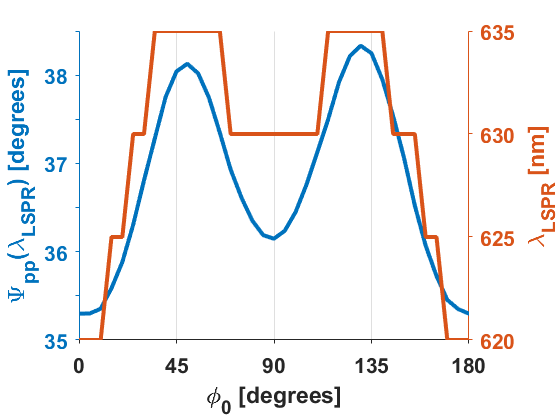
\includegraphics[width=0.9\linewidth, trim=0cm  0cm 0cm 0cm, clip]{figures/ch4/S5A/S5A_Psipp_at_LSPR(2).png}
        \caption{}
        \label{fig:S5A_LSPRvsphi_Psipp}
    \end{subfigure}
    \begin{subfigure}{0.49\textwidth}
        \centering
        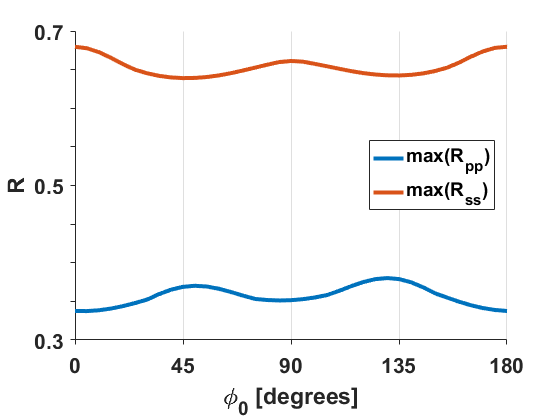
\includegraphics[width=0.9\linewidth, trim=0cm  0cm 1cm 0cm, clip]{figures/ch4/S5A/S5A_maxRpp_maxRss(1).png}
        \caption{}
        \label{fig:S5A_LSPRvsphi_RppRss}
    \end{subfigure}
    \caption{(a) Peak values of $\Psi_{pp}$ at LSPR wavelengths $\lambda_{\text{LSPR}}$ for sample 5A, plotted together with the wavelength at which the plasmon resonance peaks for a given $\phi_0$; (b) Azimuthal angle dependency of reflectances for p-polarized and s-polarized light $R_{pp}$ and $R_{ss}$, respectively, at plasmon resonance wavelengths shown in (a).}
    \label{fig:S5A_LSPRvsphi}
\end{figure}

\begin{figure}[h!]  %% Psi_ps & Psi_sp contour E and phi
    \begin{subfigure}{0.5\textwidth}
        \centering
        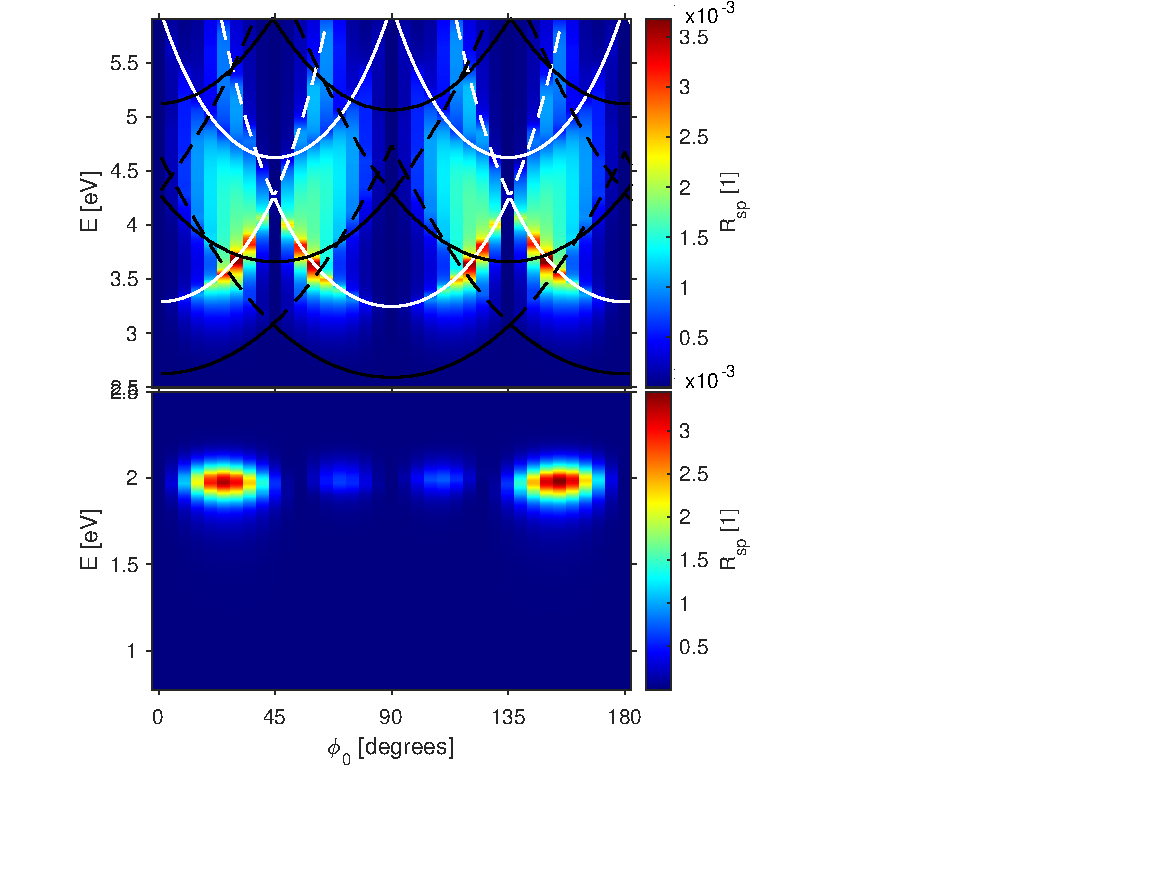
\includegraphics[width=\linewidth, trim=1.1cm  1.8cm 6.7cm 0cm, clip]{figures/ch4/S5A/contour/S5A_Rsp.pdf}
        \caption{}
    \end{subfigure}
    \begin{subfigure}{0.5\textwidth}
        \centering
        \includegraphics[width=\linewidth, trim=1.1cm  1.8cm 6.7cm 0cm, clip]{figures/ch4/S5A/contour/S5A_Rps.pdf}
        \caption{}
    \end{subfigure}

    \begin{subfigure}{0.5\textwidth}
        \centering
        \includegraphics[width=\linewidth, trim=1.1cm  1.8cm 6.7cm 0cm, clip]{figures/ch4/S5A/contour/S5A_Psisp.pdf}
        \caption{}
    \end{subfigure}
    \begin{subfigure}{0.5\textwidth}
        \centering
        \includegraphics[width=\linewidth, trim=1.1cm  1.8cm 6.7cm 0cm, clip]{figures/ch4/S5A/contour/S5A_Psips.pdf}
        \caption{}
    \end{subfigure}
    \caption{Contour plots of (a) $R_{sp}$ (b) $R_{ps}$ (c) $\Psi_{sp}$ and (d) $\Psi_{ps}$ for sample 5A. Rayleigh lines for air (white) and substrate (black) are shown in the same manner as figures \ref{fig:S5A_contour_Psipp}-d.}
    \label{fig:S5A_contour_Psips&Psisp}
\end{figure}



\begin{figure}[h!]  %% radial MM COMSOL
    \centering
    \includegraphics[width=\linewidth, trim=3cm 1.5cm 0.5cm 0cm, clip]{figures/ch4/S5A/contour/Muller_rot_S5A_COMSOLSIM_55_m21scaledtopower1over6_final.pdf}
    \caption{Contour plots of MM elements of sample 5A simulated in COMSOL with respect to photon energy $E$ and azimuthal angle $\phi_0$ of the incident light. Rayleigh lines are shown for both air (white lines) and glass substrate (black lines). Extended Rayleigh lines are included as dotted lines in elements $m_{13}$, $m_{14}$ and $m_{34}$. In $m_{21}$, reduced Rayleigh lines (i.e. boundaries of BZ) are superposed for the 1st BZ (innermost semi-square) and the 2nd BZ (tilted semi-square) can be seen for both air and substrate, as well as the 3rd BZ for SiO$_2$ (outermost black semi-square). The LSPR resonance can be seen as circles around $2$ eV. In order to more clearly observe nuances in $m_{21}$ for higher energies, a scaling has been applied for $E<2.5$ eV, in this region $|m_{12}|^{1/6}\text{sign}(m_{21})$ where $\text{sign}()$ indicates the signum function. The innermost thick-lined circle in the schematic, replacing the trivial $m_{11}$ element, corresponds to $0.78$ eV while the outer circle corresponds to $5.9$ eV.}
    \label{fig:S5A_contour_MM}
\end{figure}
\begin{figure}
    \begin{subfigure}{0.5\textwidth}
        \flushright
        \includegraphics[width=0.4\linewidth]{figures/Ch3/S5A_SEM.png}
    \end{subfigure}
    \begin{subfigure}{0.5\textwidth}
        \flushleft
        \includegraphics[width=0.33\linewidth]{figures/Ch2/ReciprocalLattice.png}
    \end{subfigure}
    \caption{SEM image of sample 5A next to a sketch of the reciprocal lattice.}
\end{figure}

\begin{figure}[h!]  %% radial MM experimental
    \centering
    \includegraphics[width=\linewidth, trim=0cm 0cm 0cm 0cm, clip]{figures/ch4/S5A/expdata/S5A_MM_rot_55.png}
    \caption{Contour plots of the elements of the \emph{experimental} normalized Mueller matrix for sample 5A as found in \cite{Brakstad:15}. The inner circle of each element corresponds to $0.73$ eV while the outer corresponds to $5.90$ eV. In element $m_{21}$, the Rayleigh lines corresponding to 1st BZ and 2nd BZ in air (white lines) and glass substrate (black lines) have been superimposed. In elements $m_{13}$ and $m_{14}$ the extended Rayleigh lines are additionally superimposed, together with a white circle at around $2.1$ eV highlighting the LSPR resonance. A scaling has been applied for elements $m_{21}$ and $m_{22}$ for energies below $2.5$ eV; in this range $m_{2j}=\text{sgn}(m_{2j})|m_{2j}|^{1/4}$, where $j=1,2$.}%
    \label{fig:S5A_contour_MM_exp}
\end{figure}
\begin{figure}[h!]
   \begin{subfigure}{0.32\linewidth}
        \centering
        \includegraphics[width=\linewidth, trim= 0cm 0cm 0cm 0cm, clip]{figures/ch4/S5A/S5A_NCS_phi0.pdf}
   \end{subfigure}
   \begin{subfigure}{0.32\linewidth}
        \centering
        \includegraphics[width=\linewidth, trim= 0cm 0cm 0cm 0cm, clip]{figures/ch4/S5A/S5A_NCS_phi25.pdf}
   \end{subfigure}
   \begin{subfigure}{0.32\linewidth}
        \centering
        \includegraphics[width=\linewidth, trim= 0cm 0cm 0cm 0cm, clip]{figures/ch4/S5A/S5A_NCS_phi45.pdf}
   \end{subfigure}
   \caption{Normalized MM elements $m_{12}$, $m_{33}$ and $m_{34}$ compared with experimental data for sample 5A.}
   \label{fig:S5A_NCS}
\end{figure}

\begin{figure}[h!] %% Psi_pp & Im(epsilon) phi0-45
    \begin{subfigure}{0.5\textwidth}
        \centering
        \includegraphics[width=\linewidth, trim=1cm 0cm 0cm 0cm, clip]{figures/ch4/S5A/S5A_Psipp_phi=0-45_offset4(1).png}
        \label{}
    \end{subfigure}
    \begin{subfigure}{0.5\textwidth}
        \centering
        \includegraphics[width=\linewidth, trim=1cm 0cm 0cm 0cm, clip]{figures/ch4/S5A/S5A_ImEpsilon_phi=0-45_offset052(2).png}
        \label{}
    \end{subfigure}
    \label{fig:S5A_Psi_Imeps_stacked}
    \caption{(a) $\Psi_{pp}$ and (b) Im$\langle\epsilon_{pp}\rangle$ for COMSOL simulated sample 5A for azimuthal angles $\phi_0 = 0^\circ-45^\circ$ in steps of $\Delta\phi_0=5^\circ$. Approximate Rayleigh lines are hand drawn in both figures. A slight dispersion of the LSPR can be seen around $2$ eV. For reasons of clarity, $\Psi_{pp}$ plots are offset by $4^\circ\kappa$ and Im$\langle\epsilon_{pp}\rangle$ by $0.52\kappa$, where $\kappa=\phi_0/\Delta\phi_0$.}
    \label{fig:S5A_stacked_PsippImeps}
\end{figure} 

\begin{figure}[h!]  %% Psi Imeps stacked over phi | experimental %% 
    \centering
    \includegraphics[width=\linewidth]{figures/ch4/S5A/expdata/S5A_Psi_Imeps_stackedphi.png}
    \caption{Experimental data of sample 5A of $\Psi_{pp}$ and Im$\langle\epsilon_{pp}\rangle$ for azimuthal angles of incidence from $\phi_0=0^\circ$ to $\phi_0=45^\circ$ in steps of $\Delta\phi_0=5^\circ$, as found in \cite{Brakstad:15}. Three approximate Rayleigh lines are hand drawn, while the location of BZ-2 in air is more unclear. $\Psi_{pp}$-curves are offset by $1.4^\circ\kappa$ and the Im$\langle\epsilon_{pp}\rangle$-curves by $0.2\kappa$, where $\kappa=\phi_0/\Delta\phi_0$. }
    \label{fig:S5A_stacked_PsippImeps_exp}
\end{figure}

\begin{figure}[h!]  %% Psi_ps & Psi_sp contour E and phi
    \centering
    \includegraphics[width=0.5\linewidth, trim=1.1cm  1.8cm 6.5cm 0cm, clip]{figures/ch4/S5A/NCS/S5A_sumNCSsquared_contour.pdf}
    \caption{Contour plot of $N^2+C^2+S^2$ for sample 5A. The sample is highly isotropic (i.e. $N^2+C^2+S^2=1$) except in regions of polarization conversion. \color{red}Obviously? Er dette interessant/verdt å ha med?}
    \label{fig:S5A_sumNCSsquared}
\end{figure}

Joule heating in terms of $P_{\text{resistive}}$ integrated over the Au particle volume is found in figure \ref{fig:S5A_heatloss}. Heat dissipation is found to be uniform up until about $2.5$ eV where it becomes highly dependent on Rayleigh lines. %Both maxima and minima follow Rayleigh lines, although (unlike figure \ref{fig:S5A_contour_Psips&Psisp}) black lines are not exclusive to maxima and white lines are not exclusive to minima

\begin{figure}[h!]  %% Resistive Heat Loss
    \begin{subfigure}{\textwidth}
        \centering
        \includegraphics[width=0.6\linewidth, trim=0cm 0cm 0cm 0cm, clip]{figures/ch4/S5A/heatloss/S5A_heat_loss_noscaling.png}
    \end{subfigure}
    
    \begin{subfigure}{\textwidth}
        \centering
        \includegraphics[width=0.5\linewidth, trim=0cm 0cm 0cm 0cm, clip]{figures/ch4/S5A/heatloss/S5A_heat_loss_phi=0,25,45(1).png}
    \end{subfigure}
    
    \caption{Top: Contour plot of resistive heat loss in units Watts over the volume of the gold particles in sample 5A, with respect to photon energy and azimuthal angle of the incident light. Rayleigh lines are indicated by solid (reduced) and dashed (extended) lines for air (white) and substrate (black). Bottom: Same plot but with the full energy spectrum for a few chosen values of $\phi_0$.}
    \label{fig:S5A_heatloss}
\end{figure}

\subsection{Field distribution}
In this section the electric field norm $E_\text{norm}$ is presented at certain wavelengths and azimuthal angles of incidence, see equation (\ref{eq:normE}). Figure \ref{fig:S5A_normE_isosurface_LSPR} visualizes the 3D field distribution of the LSPR resonance, while figure \ref{fig:S5A_normE_distribution_LSPR} plots $E_\text{norm}$ at a cross-section in the $xy$-plane located in the middle between the base of the Au particle ($z=0$) and the bottom of the mound ($z=-t$), for wavelengths surrounding the LSPR at $\phi_0=0^\circ$. As in sample 6, the LSPR is seen to be strongly concentrated around the rim of base of the Au particle at $z=0$. \text{\color{red}mer å si om LSPR?}

Figure \ref{fig:S5A_normE_phi25_z=0} attempts to show the field distribution in a spectrum of $\phi_0=25^\circ$ that has shown to exhibit polarization conversion. 

Figure \ref{fig:S5A_normE_phi0-90_wl350} shows plots of $E_\text{norm}$ in the $xy$-plane at $z=0$ for different azimuthal angles $\phi_0$ at a wavelength of relatively large polarization coupling, $\lambda=350$ nm (or $3.54$ eV). Observe that the field distribution is symmetric with respect to the plane of incidence at angles of no polarization coupling $\phi_0=0^\circ, 45^\circ, 90^\circ$, but that is not the case for $\phi_0=25^\circ, 65^\circ$.

\text{\color{red}dipole coupling?}

\begin{figure}[h!]
    \begin{subfigure}{0.5\textwidth}
        \centering
        \includegraphics[width=\linewidth, trim=0.4cm 0 1.5cm 0, clip]{figures/ch4/S5A/FieldDistribution/isosurface/Sample5A_nomE_wl620_phi0_TE.png}
        %\caption{}
    \end{subfigure}
    \begin{subfigure}{0.5\textwidth}
        \centering
        \includegraphics[width=\linewidth, trim=0.6cm 0 1.6cm 0, clip]{figures/ch4/S5A/FieldDistribution/isosurface/Sample5A_nomE_wl620_phi0_TM.png}
        %\caption{}
    \end{subfigure}
    
    \begin{subfigure}{0.5\textwidth}
        \centering
        \includegraphics[width=\linewidth, trim=0.6cm 0 1.6cm 0, clip]{figures/ch4/S5A/FieldDistribution/isosurface/Sample5A_nomE_wl620_phi0_TE_xoutofpaper.png}
        \caption{TE}
    \end{subfigure}
    \begin{subfigure}{0.5\textwidth}
        \centering
        \includegraphics[width=\linewidth, trim=0.6cm 0 1.6cm 0, clip]{figures/ch4/S5A/FieldDistribution/isosurface/Sample5A_nomE_wl620_phi0_TM_yintopaper.png}
        \caption{TM}
    \end{subfigure}
    \caption{The electric field norm $E_\text{norm}$ plotted for five layers of isosurface when incident wave is (a) TE polarized and (b) TM polarized at wavelength $\lambda_{\text{LSPR}}=620$ nm and azimuthal angle $\phi_0=0^\circ$, i.e. propagating along $\hat{x}$-direction at polar incidence $\theta_0=55^\circ$. Two viewpoints of each plot is given: a general view for both (top), $\hat{x}$ is pointing out of paper for TE (bottom left), and $\hat{y}$ is pointing into paper for TM (bottom right).}
    \label{fig:S5A_normE_isosurface_LSPR}
\end{figure}


\begin{figure}[htb!]  %% FIELD DISTRIBUTION 575-725 nm
    \begin{subfigure}{0.32\textwidth}    %% TE
        \centering
        \includegraphics[width=\linewidth]{figures/ch4/S5A/FieldDistribution/LSPR/Sample5A_TE_Slice@z=-05t_wl=575_notitle.png}
        %\caption{}
   \end{subfigure}
   \begin{subfigure}{0.32\textwidth}
        \centering
        \includegraphics[width=\linewidth]{figures/ch4/S5A/FieldDistribution/LSPR/Sample5A_TE_Slice@z=-05t_wl=600_notitle.png}
        %\caption{}
   \end{subfigure}
   \begin{subfigure}{0.32\textwidth}
        \centering
        \includegraphics[width=\linewidth]{figures/ch4/S5A/FieldDistribution/LSPR/Sample5A_TE_Slice@z=-05t_wl=620_notitle.png}
        %\caption{}
   \end{subfigure}

    \begin{subfigure}{0.32\textwidth}
        \centering
        \includegraphics[width=\linewidth]{figures/ch4/S5A/FieldDistribution/LSPR/Sample5A_TE_Slice@z=-05t_wl=640_notitle.png}
        %\caption{}
   \end{subfigure}
   \begin{subfigure}{0.32\textwidth}
        \centering
        \includegraphics[width=\linewidth]{figures/ch4/S5A/FieldDistribution/LSPR/Sample5A_TE_Slice@z=-05t_wl=675_notitle.png}
        \caption{TE}
        \vspace{-0.7cm}
   \end{subfigure}
   \begin{subfigure}{0.32\textwidth}
        \centering
        \includegraphics[width=\linewidth]{figures/ch4/S5A/FieldDistribution/LSPR/Sample5A_TE_Slice@z=-05t_wl=725_notitle.png}
        %\caption{}
   \end{subfigure}
   \vspace{0.7cm}
   
   \begin{subfigure}{0.32\textwidth}    %% TM
        \centering
        \includegraphics[width=\linewidth]{figures/ch4/S5A/FieldDistribution/LSPR/Sample5A_TM_Slice@z=-05t_wl=575_notitle.png}
        %\caption{}
   \end{subfigure}
      \begin{subfigure}{0.32\textwidth}
        \centering
        \includegraphics[width=\linewidth]{figures/ch4/S5A/FieldDistribution/LSPR/Sample5A_TM_Slice@z=-05t_wl=600_notitle.png}
        %\caption{}
   \end{subfigure}
    \begin{subfigure}{0.32\textwidth}
        \centering
        \includegraphics[width=\linewidth]{figures/ch4/S5A/FieldDistribution/LSPR/Sample5A_TM_Slice@z=-05t_wl=620_notitle.png}
        %\caption{}
   \end{subfigure}
   
   
    \begin{subfigure}{0.32\textwidth}
        \centering
        \includegraphics[width=\linewidth]{figures/ch4/S5A/FieldDistribution/LSPR/Sample5A_TM_Slice@z=-05t_wl=640_notitle.png}
        %\caption{}
        %\vspace{-1cm}
   \end{subfigure}
   \begin{subfigure}{0.32\textwidth}
        \centering
        \includegraphics[width=\linewidth]{figures/ch4/S5A/FieldDistribution/LSPR/Sample5A_TM_Slice@z=-05t_wl=675_notitle.png}
        \caption{TM}
        \vspace{-0.7cm}
   \end{subfigure}   
   \begin{subfigure}{0.32\textwidth}
        \centering
        \includegraphics[width=\linewidth]{figures/ch4/S5A/FieldDistribution/LSPR/Sample5A_TM_Slice@z=-05t_wl=725_notitle.png}
        %\caption{}
        %\vspace{-1cm}
   \end{subfigure}
   \vspace{0.7cm}
   \caption{Electric field norm $E_{\text{norm}}$ at increasing wavelengths between 575-725 nm distributed over sample 5A at a cross-section in xy-plane located at $z=-t/2$, as seen from the top of air domain and down towards the gold particle and substrate. The inner black circle marks the edges of the particle at $z=0$, while the outer border-less circle indicate the mound cut right at the middle of its height. (a) shows the electric field norm when the incident light is TE polarized with azimuthal angle $\phi_0=0^\circ$, i.e. beam incident in +x-direction. Similar in (b) for TM-polarization. For both figures, from top left to bottom right in (a) and (b), the electric field distribution is shown subsequentially for wavelengths $\lambda_0=575 \text{nm}, 600 \text{nm}, 620 \text{nm}, 640 \text{nm}, 675 \text{nm}, 725 \text{nm}$. Axis directions are marked in the bottom left corner of each sub-figure. The colorbar marks the values for $E_{\text{norm}}$ in units V/m.}
   \label{fig:S5A_normE_distribution_LSPR}
\end{figure}



\begin{figure}[htb!]  
    \begin{subfigure}{0.32\textwidth}    %% TE
        \centering
        \includegraphics[width=\linewidth]{figures/ch4/S5A/FieldDistribution/phi25/Sample5A_TE_Slice@z=0_wl=230_phi=25.png}
        %\caption{}
   \end{subfigure}
   \begin{subfigure}{0.32\textwidth}
        \centering
        \includegraphics[width=\linewidth]{figures/ch4/S5A/FieldDistribution/phi25/Sample5A_TE_Slice@z=0_wl=255_phi=25.png}
        %\caption{}
   \end{subfigure}
   \begin{subfigure}{0.32\textwidth}
        \centering
        \includegraphics[width=\linewidth]{figures/ch4/S5A/FieldDistribution/phi25/Sample5A_TE_Slice@z=0_wl=300_phi=25.png}
        %\caption{}
   \end{subfigure}

    \begin{subfigure}{0.32\textwidth}
        \centering
        \includegraphics[width=\linewidth]{figures/ch4/S5A/FieldDistribution/phi25/Sample5A_TE_Slice@z=0_wl=350_phi=25.png}
        %\caption{}
   \end{subfigure}
   \begin{subfigure}{0.32\textwidth}
        \centering
        \includegraphics[width=\linewidth]{figures/ch4/S5A/FieldDistribution/phi25/Sample5A_TE_Slice@z=0_wl=400_phi=25.png}
        \caption{TE}
        \vspace{-0.7cm}
   \end{subfigure}
   \begin{subfigure}{0.32\textwidth}
        \centering
        \includegraphics[width=\linewidth]{figures/ch4/S5A/FieldDistribution/phi25/Sample5A_TE_Slice@z=0_wl=500_phi=25.png}
        %\caption{}
   \end{subfigure}
   \vspace{0.7cm}
   
    \begin{subfigure}{0.32\textwidth}    %% TM
        \centering
        \includegraphics[width=\linewidth]{figures/ch4/S5A/FieldDistribution/phi25/Sample5A_TM_Slice@z=0_wl=230_phi=25.png}
        %\caption{}
   \end{subfigure}
   \begin{subfigure}{0.32\textwidth}
        \centering
        \includegraphics[width=\linewidth]{figures/ch4/S5A/FieldDistribution/phi25/Sample5A_TM_Slice@z=0_wl=255_phi=25.png}
        %\caption{}
   \end{subfigure}
   \begin{subfigure}{0.32\textwidth}
        \centering
        \includegraphics[width=\linewidth]{figures/ch4/S5A/FieldDistribution/phi25/Sample5A_TM_Slice@z=0_wl=300_phi=25.png}
        %\caption{}
   \end{subfigure}

    \begin{subfigure}{0.32\textwidth}
        \centering
        \includegraphics[width=\linewidth]{figures/ch4/S5A/FieldDistribution/phi25/Sample5A_TM_Slice@z=0_wl=350_phi=25.png}
        %\caption{}
   \end{subfigure}
   \begin{subfigure}{0.32\textwidth}
        \centering
        \includegraphics[width=\linewidth]{figures/ch4/S5A/FieldDistribution/phi25/Sample5A_TM_Slice@z=0_wl=400_phi=25.png}
        \caption{TM}
        \vspace{-0.7cm}
   \end{subfigure}
   \begin{subfigure}{0.32\textwidth}
        \centering
        \includegraphics[width=\linewidth]{figures/ch4/S5A/FieldDistribution/phi25/Sample5A_TM_Slice@z=0_wl=500_phi=25.png}
        %\caption{}
   \end{subfigure}
   \vspace{0.7cm}
   
   \begin{subfigure}{0.5\textwidth}
        \centering
        \includegraphics[scale=0.28]{figures/ch4/S5A/FieldDistribution/phi25/S5A_rpp_rss_phi25.png}
    \end{subfigure}
    \begin{subfigure}{0.5\textwidth}
        \centering
        \includegraphics[scale=0.28]{figures/ch4/S5A/FieldDistribution/phi25/S5A_rsp_rps_phi25.png}
    \end{subfigure}
   \caption{Electric field norm distribution of sample 5A at a cross section in the xy-plane located at $z=0$ (i.e. at bottom base of Au particle) at wavelengths $\lambda_0=230$nm, $255$nm, $300$nm, $350$nm, $400$nm, $500$nm and azimuthal incident angle $\phi_0=25^\circ$. Reflectance plots of the relevant spectrum and $\phi_0$ is included below.}
   \label{fig:S5A_normE_phi25_z=0}   
\end{figure}



\begin{figure}[htb!]  
    \begin{subfigure}{0.32\textwidth}    %% TE
        \centering
        \includegraphics[width=\linewidth]{figures/ch4/S5A/FieldDistribution/phi0-90/Sample5A_TE_Slice@z=0_wl=350_phi=0.png}
        %\caption{}
   \end{subfigure}
   \begin{subfigure}{0.32\textwidth}
        \centering
        \includegraphics[width=\linewidth]{figures/ch4/S5A/FieldDistribution/phi0-90/Sample5A_TE_Slice@z=0_wl=350_phi=25.png}
        %\caption{}
   \end{subfigure}
   \begin{subfigure}{0.32\textwidth}
        \centering
        \includegraphics[width=\linewidth]{figures/ch4/S5A/FieldDistribution/phi0-90/Sample5A_TE_Slice@z=0_wl=350_phi=45.png}
        %\caption{}
   \end{subfigure}

    \begin{subfigure}{0.32\textwidth}
        \centering
        \includegraphics[width=\linewidth]{figures/ch4/S5A/FieldDistribution/phi0-90/Sample5A_TE_Slice@z=0_wl=350_phi=65.png}
        %\caption{}
   \end{subfigure}
   \begin{subfigure}{0.32\textwidth}
        \centering
        \includegraphics[width=\linewidth]{figures/ch4/S5A/FieldDistribution/phi0-90/Sample5A_TE_Slice@z=0_wl=350_phi=90.png}
        \caption{TE}
        \vspace{-0.7cm}
   \end{subfigure}
   \begin{subfigure}{0.32\textwidth}
        \centering
        \includegraphics[width=\linewidth]{figures/ch4/S5A/FieldDistribution/phi0-90/S5A_rps_phi0-90.png}
        %\caption{}
   \end{subfigure}
   \vspace{0.7cm}
   
    \begin{subfigure}{0.32\textwidth}    %% TM
        \centering
        \includegraphics[width=\linewidth]{figures/ch4/S5A/FieldDistribution/phi0-90/Sample5A_TM_Slice@z=0_wl=350_phi=0.png}
        %\caption{}
   \end{subfigure}
   \begin{subfigure}{0.32\textwidth}
        \centering
        \includegraphics[width=\linewidth]{figures/ch4/S5A/FieldDistribution/phi0-90/Sample5A_TM_Slice@z=0_wl=350_phi=25.png}
        %\caption{}
   \end{subfigure}
   \begin{subfigure}{0.32\textwidth}
        \centering
        \includegraphics[width=\linewidth]{figures/ch4/S5A/FieldDistribution/phi0-90/Sample5A_TM_Slice@z=0_wl=350_phi=45.png}
        %\caption{}
   \end{subfigure}

    \begin{subfigure}{0.32\textwidth}
        \centering
        \includegraphics[width=\linewidth]{figures/ch4/S5A/FieldDistribution/phi0-90/Sample5A_TM_Slice@z=0_wl=350_phi=65.png}
        %\caption{}
   \end{subfigure}
   \begin{subfigure}{0.32\textwidth}
        \centering
        \includegraphics[width=\linewidth]{figures/ch4/S5A/FieldDistribution/phi0-90/Sample5A_TM_Slice@z=0_wl=350_phi=90.png}
        \caption{TM}
        \vspace{-0.7cm}
   \end{subfigure}
   \begin{subfigure}{0.32\textwidth}
        \centering
        \includegraphics[width=\linewidth]{figures/ch4/S5A/FieldDistribution/phi0-90/S5A_rsp_phi0-90.png}
        %\caption{}
   \end{subfigure}
   \vspace{0.7cm}
   \caption{Electric field norm of sample 5A at wavelength $\lambda_0=350$ nm and azimuthal angles of incidence $\phi_0=0^\circ, 25^\circ, 45^\circ, 65^\circ, 90^\circ$ when the incident beam is (a) TE- and (b) TM-polarized. The cross-section is located at the base of the Au particle, $z=0$.}
   \label{fig:S5A_normE_phi0-90_wl350}   
\end{figure}











\clearpage


Plots: stackedMM (appendix?).

\clearpage
%%%%%%%%%%%%%%% new sub section %%%%%%%%%%%%%%%
\subsection{Comparing changes in lattice constants and particle ellipticity}
\label{sec:results_S5A_comparisons}
This section will investigate the effect of sample 5A's non-uniform lattice constants and particle lateral parameters, in particular how they shape the LSPR resonance strength and wavelength position. Three models with similar geometry to sample 5A have been simulated; a completely uniform structure with square lattice and circular base of the Au particle; a structure with circular particle base but very rectangular lattice; lastly a structure with slightly elliptic Au particles and square lattice. The parameters for these are summarized in table \ref{tab:S5A_comparisons}, where sample 5A parameters are repeated for convenience. The models were simulated in COMSOL for wavelengths $\lambda=500-800$ nm and incident azimuthal angles $\phi_0=0^\circ-180^\circ$ in stepsizes of $5$ nm and $5^\circ$, respectively, and incident polar angle the usual $\theta_0=55^\circ$.
\begin{table}[h]
\centering
\caption{All quantities are given in nanometers.}
\label{tab:S5A_comparisons}
\begin{tabular}{l l l l l}
            &   Uniform    &   Rectangular lattice   &   Ellipsoidal Au   & Sample 5A\\
    \hline 
    $a_x$   &   208.6      &   198.6           &   208.6    &   207.2       \\
    $a_y$   &   208.6       &   218.6           &   208.6   &   209.9  \\
    $R_x$   &   60.8           &   60.8           &   60.3  &   60.3     \\
    $R_y$   &   60.8           &   60.8           &   61.3  &   61.3 \\
    $R_z$   &   34.8           &   34.8           &   34.8  &   34.8    \\
    $t$     &   36.9           &   36.9           &   36.9  &   36.9    \\
    \hline
\end{tabular}
\end{table}

The main results of these simulations are found in figure \ref{fig:S5A_comparisons_Psipp@LSPR}, where peak $\Psi_{pp}$ and the LSPR wavelength $\lambda_\text{LSPR}$ is plotted with respect to incident azimuthal angle. The reader is reminded that $\phi_0=0^\circ$ is defined along the x-axis. It is immediately observed that sample 5A follow closely the profile of the ellipsoidal particle. Sample 5A is seen to slightly shift towards the rectangular lattice profile at the extreme points of $\Psi_{pp}(\lambda_\text{LSPR})$, suggesting that its non-uniform lattice constants do have an effect, albeit small. In fact, in order for the rectangular lattice model to have noticeable effect on the LSPR, the lattice constants $a_x$, $a_y$ had to be exaggerated compared to the estimated sample 5A parameters.  Note that none of the models display a perfect $90^\circ$ symmetry, not even the uniform sample where one might expect a $45^\circ$ symmetry. Experimental data in figure \ref{fig:S5A_comparisons_Psipp@LSPR_expdata} seem to inherit a symmetry similar to that of the ellipsoidal particle in figures \ref{fig:S5A_comparisons_Psipp@LSPR}.

\begin{figure}[h]
    \begin{subfigure}{0.5\textwidth}
        \centering
        \includegraphics[width=\linewidth]{figures/ch4/S5A/comparisons/comparisons_Psipp_at_LSPR.pdf}
        \caption{}
        \label{}
    \end{subfigure}
    \begin{subfigure}{0.5\textwidth}
        \centering
        \includegraphics[width=\linewidth]{figures/ch4/S5A/comparisons/comparisons_wl@LSPR.pdf}
        \caption{}
        \label{}
    \end{subfigure}
    \caption{Plots comparing models of Sample 5A with slightly different unit cell parameters; an exaggerated rectangular lattice with circular hemispheroidal gold particle; an ellipsoidal gold particle with square lattice; and a uniform model with hemispheroidal particle and square lattice. (a) Values of $\Psi_{pp}$ at the peak LSPR resonance located at $\lambda_{\text{LSPR}}$, (b) illustrates how this wavelength shifts with respect to incident azimuthal angle $\psi_0$. Results of the original Sample 5A simulation, as in figure \ref{fig:S5A_LSPRvsphi_Psipp}, is also plotted (dash-dotted black line).}
    \label{fig:S5A_comparisons_Psipp@LSPR}
\end{figure}
\begin{figure}[h]
    \centering
    \includegraphics[width=0.5\linewidth]{figures/ch4/S5A/comparisons/S5Aexperimental_Psipp_at_LSPR.pdf}
    \caption{Experimental data of sample 5A revealing anisotropy of peak LSPR resonance with regards to wavelength and azimuthal angle of the incident light.}
    \label{fig:S5A_comparisons_Psipp@LSPR_expdata}
\end{figure}

The plasmonic properties of elongated gold particles (or nanorods) have been studied extensively the last decade\cite{Au_nanorods_review}\cite{LSPR_sensor_review}. In particular the sensitive nature of plasmon resonances to their shape and orientation\cite{multipolePlasmons_metalrods}. Figure \ref{fig:S5A_comparison_Psi_ellipticity} shows how $\Psi_{pp}$ evolves into two separate LSPRs at $\phi_0=0^\circ$ and $\phi_0=90^\circ$ as the ellipticity of the Au particle increases. The resonance peak at $\phi_0=0^\circ$ is blueshifted from $620$ nm to a smaller peak at $580$ nm where reflected s-polarized light dominates, while the resonance at $\phi_0=90^\circ$ is redshifted from $630$ nm to a stronger peak at $665$ nm where most of the light reflected from the sample is p-polarized. This is in agreement with the intuition that light incident along the x-axis would experience a wider particle and thus strongly resonate with the s-polarized light, and similar for y-direction where light intuitively experiences a narrow but long Au particle that resonate with the p-polarization.

\begin{figure}[h!]
    \begin{subfigure}{0.5\textwidth}
        \centering
        \includegraphics[width=\linewidth]{figures/ch4/S5A/comparisons/Psipp_vs_lambda_vs_phi_Rx605_Ry615_Rz348_t369_axy209_theta55.png}
    \end{subfigure}
    \begin{subfigure}{0.5\textwidth}
        \centering
        \includegraphics[width=\linewidth]{figures/ch4/S5A/comparisons/Psipp_vs_lambda_vs_phi_Rx59_Ry63_Rz348_t369_axy209_theta55.png}
    \end{subfigure}
    
    \begin{subfigure}{0.5\textwidth}
        \centering
        \includegraphics[width=\linewidth]{figures/ch4/S5A/comparisons/Psipp_vs_lambda_vs_phi_Rx56_Ry66_Rz348_t369_axy209_theta55.png}
    \end{subfigure}
    \begin{subfigure}{0.5\textwidth}
        \centering
        \includegraphics[width=\linewidth]{figures/ch4/S5A/comparisons/Psipp_vs_lambda_vs_phi_Rx51_Ry71_Rz348_t369_axy209_theta55.png}
    \end{subfigure}
    \caption{Variations of sample 5A parameters with increasing ellipticity of the gold particle, as marked in each subfigure. Common parameters for all four cases are the particle height $R_z=34.8$nm, mound height $t=36.9$nm, square lattice $a_{xy}=209$nm and incident polar angle $\theta_0=55^\circ$. Azimuthal angle $\phi_0=0^\circ$ is defined along x-axis, while $\phi_0=90^\circ$ corresponds to light incident in positive y-direction.}
    \label{fig:S5A_comparison_Psi_ellipticity}
\end{figure}

\clearpage
%%%%%%%%%%%%%%% NEW SECTION %%%%%%%%%%%%%%%
\section{Sample 5B}
Sample 5B has very large lattice constants ($a_x=315.4$ nm, $a_y=443.9$ nm) compared to the spectrum of interest ($\lambda=210-1700$ nm) thus creating a very large volume for the computational domain. As previously stated in section \ref{sec:ch3_sample5B}, the dielectric mound (with a height estimated at around $15$ nm) was not included in the simulated geometry. Even so, the desktop computer was not able to solve the model for the lower wavelengths due to the large amount of mesh elements. The lowest wavelength resulting in a solvable mesh was $250$ nm, i.e. the simulated region is $\lambda=250-1700$ nm where each wavelength is swept for azimuthal angles $\phi_0=0^\circ-180^\circ$. TE and TM simulations were not be able to run simultaneously on the desktop computer due to the computationally demanding calculations. The program used at most $23.4$ GB RAM, which was during full wave calculation of the lowest wavelength, $250$ nm, solved in 2 hours and 18 minutes in real-time. The solution time for each increasing wavelength decreased exponentially, finally solving for $1700$ nm in just under 2 minutes. The total wall time, including both TE and TM simulations, was 94 hours and 59 minutes, where over $82\%$ of this time was spent solving for wavelengths in the region $250-900$ nm. Multiplying the wall time by the number of CPU cores gives us an approximate CPU time of 23 days 17 hours and 54 minutes. 
\begin{itemize}

    \item Feltfordeling rundt Rayleigh-linjer? COMSOL figurer?
    \item Dipolkopling?
    \item Rayleigh lines go deep into LSPR region. Consequences? Sharper resonance? Figure \ref{fig:S5B_contourEpsilonPsipp} seem to agree with this. LSPR resonances seem to "avoid" nearby Rayleigh lines, forcing sharper peaks and maybe even splitting a peak? See $\Psi_pp$ at $90$ degrees at $1.8$ eV.
    \item Split into two LSPRs, one weak at 2 eV for $\phi_0$ and another stronger resonance between 1.2-1.6 eV.
\end{itemize}

\begin{figure}[h]  %% Rss Rpp Psipp contour E and phi
    \begin{subfigure}{0.5\textwidth}
        \centering
        \includegraphics[width=\linewidth, trim=1.2cm  1.8cm 6.5cm 0.3cm, clip]{figures/ch4/S5B/contour/S5B_Rpp.pdf}
        \caption{}
        \label{fig:S5B_contour_Rpp}
    \end{subfigure}
    \begin{subfigure}{0.5\textwidth}
        \centering
        \includegraphics[width=\linewidth, trim=1.2cm  1.8cm 6.5cm 0.3cm, clip]{figures/ch4/S5B/contour/S5B_Rss.pdf}
        \caption{}
        \label{fig:S5B_contour_Rss}
    \end{subfigure}
    
    \begin{subfigure}{0.5\textwidth}
        \centering
        \includegraphics[width=\linewidth, trim=1.2cm  1.8cm 6.5cm 0.3cm, clip]{figures/ch4/S5B/contour/S5B_Psipp.pdf}
        \caption{}
    \end{subfigure}
    \begin{subfigure}{0.5\textwidth}
        \centering
        \begin{subfigure}{\textwidth}
            \centering
            \includegraphics[width=0.41\linewidth]{figures/Ch3/s5b/S5B_schematic.png}
        \end{subfigure}
        
        \begin{subfigure}{\textwidth}
            \centering
            \includegraphics[width=0.5\linewidth]{figures/Ch2/ReciprocalLattice.png}
        \end{subfigure}
        %\caption{}
    \end{subfigure}
    
    \caption{Contour plots of (a) $R_{pp}$ (b) $R_{ss}$ and (c) $\Psi_{pp}$ for sample 5B. For reasons of improved visibility, energies above $2.5$ eV have independent colorbars. Rayleigh lines are shown corresponding to the boundaries of BZ-1 ($\mathbf{G}_\parallel^{\bar{1}0}$), BZ-2 ($\mathbf{G}_\parallel^{\bar{1}\bar{1}}$) and BZ-3 ($\mathbf{G}_\parallel^{\bar{2}0}$) for air (white) and glass substrate (black). In addition, extended Rayleigh lines for the 1st BZs for both air and glass are shown in dashed lines. Brillouin zones with reciprocal lattice vectors $\mathbf{G}_\parallel^{\bar{1}\bar{1}}$ for air and substrate are recognized by their $45^\circ$ symmetry, while the others are symmetric around $90^\circ$.}
    \label{fig:S5B_contour_RppRss_Psipp}
\end{figure}

\begin{figure}
    \begin{subfigure}{0.5\textwidth}
    \begin{subfigure}{\textwidth}
        \centering
        \includegraphics[width=0.9\linewidth]{figures/ch4/S5B/fielddistr/s5b_normE_TM_wl1010_phi90(2).png}
    \end{subfigure}
    
    \begin{subfigure}{\textwidth}
        \centering
        \includegraphics[width=0.9\linewidth]{figures/ch4/S5B/fielddistr/s5b_normE_TM_wl1010_phi90(1).png}
    \end{subfigure}
    \caption{TM}
    \end{subfigure}
    \begin{subfigure}{0.5\textwidth}
    \begin{subfigure}{\textwidth}
        \centering
        \includegraphics[width=0.9\linewidth]{figures/ch4/S5B/fielddistr/s5b_normE_TE_wl1010_phi90.png}
    \end{subfigure}
    
    \begin{subfigure}{\textwidth}
        \centering
        \includegraphics[width=0.9\linewidth]{figures/ch4/S5B/fielddistr/s5b_normE_TE_wl1010_phi90(1).png}
    \end{subfigure}
    \caption{TE}
    \end{subfigure}
    \caption{Field distribution around the gold particles of sample 5B when the incident beam has wavelength $\lambda=1010$ nm ($1.23$ eV) and azimuthal angle $\phi_0=90^\circ$ polarized (a) longitudinal and (b) transversal to the plane of incidence, where each plot is given at two different viewpoints (top and bottom). The field amplitude $E_\text{norm}$ is plotted for seven layers of isosurfaces given in SI units V$/$m.}
    \label{fig:S5B_fielddstribution_LSPR_phi90}
\end{figure}

Contour plots of the optical response of the reflected COMSOL sample are given in figure \ref{fig:S5B_contour_RppRss_Psipp} as $R_{pp}$, $R_{ss}$ and $\Psi_{pp}$. A SEM image of the experimental sample together with a schematic of the reciprocal (square!) lattice defining the azimuthal angle of incidence is repeated, for convenience. Figure \ref{fig:S5B_contour_Rss} reveal a resonance around $1.4$ eV excited by the transverse mode incident along the x-axis, and a very small resonance at $\phi_0=90^\circ$ around $2.1$ eV. The longitudinal mode seen in figure \ref{fig:S5B_contour_Rpp} excites two plasmon resonances along the y-axis: a weak resonance sharply defined at $1.9$ eV and a strong resonance between $1.20-1.54$ eV which is confined between the Rayleigh lines corresponding to the 1st BZs of SiO$_2$ and air. There is also observed a very weak resonance along the x-axis around $2.1$ eV. The field distributions for both modes at the strong LSPR located at photon energy $1.23$ eV with $\phi_0=90^\circ$ can be found in figure \ref{fig:S5B_fielddstribution_LSPR_phi90}. Notice a factor 10 difference in field strength between TM and TE polarizations, where values for $R_{pp}$ and $R_{ss}$ at the same location is $0.20$ and $0.128$, respectively, confirming an enhanced field when the incident light is polarized along the semi-major axis of a particle with high aspect ratio.

As a consequence of the large lattice constants the Rayleigh lines for the 1st BZ go deep into the LSPR region of the particles. These are seen to sharply define the edges of the resonance located at $\phi_0=90^\circ$ in $R_{pp}$, while the 1st BZ in glass also seem to dampen the $R_{ss}$ resonance at the $X$-point.

In figure \ref{fig:S5B_N@LSPR} the position of peak resonances are plotted with respect to incident angle. Here, MM element $m_{12}$ is used as it is similar in profile to $\Psi_{pp}$ but with features more sharply defined.

Seeing as the LSPR is consentrated along the rim base of the Au particles in direct contact with the substrate, they may be subject to the dispersive SiO$_2$ refractive index which varies from $1.514$ to $1.446$ in the simulated region. It has been shown that gold nanoparticles with high aspect ratios are extremely sensitive to the ambient refractive index, where the longitudinal LSPR peak redshifts as the refractive index increases and the shift amplitude inreases with the aspect ratio\cite{LSPR_sensor_review}\cite{Au_nanorods_review}. It could be interesting to compare these results with a similar simulation using a glass substrate with constant refractive index, which could be source for future work.

For energies above $2.5$ eV the sample is highly isotropic, as the reflection MM resembles equation (\ref{eq:isotropicMM}) and the majority of light is transmitted through the glass (transmission results not shown). There is a very weak polarization coupling present for $E>2.5$ eV, as seen in figure \ref{fig:S5B_contour_Rsp&Rps_Psisp&Psips}, which to a certain extent seem to follow the Rayleigh lines for air, particularly the extended lines for $\mathbf{G}_\parallel^{\bar{1}0}$. This weak conversion of polarization is also visible in the upper off-block-diagonal elements in figure \ref{fig:S5B_contour_MM} where a scaling has been applied to improve visibility.



The experimental MM is found in figure \ref{fig:S5B_contour_MM_exp}. Note that the off-diagonal MM elements of the experimental sample are overall larger than its COMSOL counterpart. This suggest a structure-induced anisotropy caused by the dielectric mound, which has been neglected in the simulation.



\begin{figure}[h]
    \begin{subfigure}{0.65\textwidth}
        \centering
        \includegraphics[width=\linewidth, trim=0cm 0cm 0.6cm 0cm, clip]{figures/ch4/S5B/LSPR/N_contour(1).png}
        \caption{}
        \label{}
    \end{subfigure}
    \begin{subfigure}{0.34\textwidth}
        \centering
        \includegraphics[width=0.5\linewidth]{figures/Ch3/s5b/S5B_schematic.png}
    \end{subfigure}
    
    \begin{subfigure}{0.49\textwidth}
        \centering
        \includegraphics[width=\linewidth]{figures/ch4/S5B/LSPR/N@LSPR(2).png}
        \caption{}
        \label{}
    \end{subfigure}
    \begin{subfigure}{0.49\textwidth}
        \centering
        \includegraphics[width=\linewidth]{figures/ch4/S5B/LSPR/RppRss@LSPR.png}
        \caption{}
        \label{}
    \end{subfigure}
    \caption{[placeholder caption Sample 5B] (a) corresponds to $m_{12}$ element of the MM in figure \ref{fig:S5B_contour_MM}. Large resonance centered at $\phi_0=90^\circ$, as well as several noticeable peaks around 600 nm at $\phi_0=0^\circ,90^\circ,180^\circ$. A dip between the two resonances at $90^\circ$ is observed at 700 nm; (b) peak values of N at the resonance wavelengths $\lambda_{\text{LSPR}}$ (blue), together with $\lambda_{\text{LSPR}}$ positions (red) with respect to azimuthal angle. An attempt to separate the two resonances at $90^\circ$ has been done by plotting quantities below the minimum at 700 nm (dotted lines) and above (solid lines). The discontinuity at 700 nm shows that at $\phi_0=25^\circ,155^\circ$ the main resonance has dwindled off in strength to the point that the smaller resonances at around 635 nm have surpassed it.}
    \label{fig:S5B_N@LSPR}
\end{figure}

\begin{figure}[h]  %% radial MM
    \centering
    \includegraphics[width=\linewidth, trim=3cm 1cm 0.4cm 0cm, clip]{figures/ch4/S5B/contour/Muller_rot_S5B_COMSOLSIM_55_final(2).pdf}
    \caption{Contour plots of the normalized Mueller matrix elements for sample 5B. Energy and azimuthal angle of the incident light are represented by radius and rotation angle in each polar plot, respectively. Inner circle of the schematic in $m_{11}$ corresponds to photon energy 0.73 eV while the outermost circle corresponds to 4.96 eV. Scaling has been applied to a few elements, for reasons of improved clarity in energy regions above 2.3 eV; Resonant values in the upper off-block elements $m_{13}$, $m_{14}$, $m_{23}$ and $m_{24}$ were reduced by $|m_{ij}|^{1/4}\text{sign}(m_{ij})$ and similar for $m_{22}$, while element $m_{21}=m_{12}$ has been set completely void for energies below 2.35 eV. Furthermore, in $m_{44}$, reduced Rayleigh lines are drawn for air (white lines) and glass substrate (black lines). For glass, the first four Brillouin zones can be seen in this element, as well as parts of BZ-5 ($\mathbf{G}_\parallel^{\bar{3}0}$) . The first BZ can be seen as the innermost upright rectangle, BZ-2 is the tilted semi-square, BZ-3 is again an upright semi-rectangle but larger, while BZ-4  ($\mathbf{G}_\parallel^{\bar{2}\bar{2}}$) is the largest tilted semi-square. In elements $m_{23}$ and $m_{24}$, the extended Rayleigh lines (dotted lines) are also included for air and substrate, respectively. Lastly, in element $m_{21}$ all Rayleigh lines (excluding BZ-1) for both air and substrate are superimposed.} 
    \label{fig:S5B_contour_MM_exp}
    % BZ1 (10) BZ2 (11) BZ3 (20) BZ4 (22)
\end{figure}

\begin{figure}[h]  %% radial MM exp
    \centering
    \includegraphics[width=\linewidth, trim=3cm 1cm 0.5cm 0cm, clip]{figures/ch4/S5B/exp/S5B_MM_exp_55.pdf}
    \caption{Contour plot of the MM elements of the experimental sample 5B measured at $\theta_0=55^\circ$. Inner circle correspond to $0.73$ eV while the outer circle is $5.9$ eV.} 
    \label{fig:S5B_contour_MM}
    % BZ1 (10) BZ2 (11) BZ3 (20) BZ4 (22)
\end{figure}
\begin{figure}[h!]
   \begin{subfigure}{0.32\linewidth}
        \centering
        \includegraphics[width=\linewidth, trim= 0cm 0cm 2cm 0cm, clip]{figures/ch4/S5B/NCS/S5B_NCS_phi0.pdf}
   \end{subfigure}
   \begin{subfigure}{0.32\linewidth}
        \centering
        \includegraphics[width=\linewidth, trim= 0cm 0cm 2cm 0cm, clip]{figures/ch4/S5B/NCS/S5B_NCS_phi45.pdf}
   \end{subfigure}
   \begin{subfigure}{0.32\linewidth}
        \centering
        \includegraphics[width=\linewidth, trim= 0cm 0cm 2cm 0cm, clip]{figures/ch4/S5B/NCS/S5B_NCS_phi90.pdf}
   \end{subfigure}
   \caption{Normalized MM elements $m_{12}$, $m_{33}$ and $m_{34}$ compared with experimental data for sample 5B at three chosen angles of azimuthal incidence.}
   \label{fig:S5A_NCS}
\end{figure}




\begin{figure}[h]  %% Psi_ps & Psi_sp contour E and phi %% 
    \begin{subfigure}{0.49\textwidth}
        \centering
        \includegraphics[width=\linewidth, trim=1.2cm  1.8cm 6.5cm 0.3cm, clip]{figures/ch4/S5B/contour/S5B_Rsp.pdf}
        \caption{}
    \end{subfigure}
    \begin{subfigure}{0.49\textwidth}
        \centering
        \includegraphics[width=\linewidth, trim=1.2cm  1.8cm 6.5cm 0.3cm, clip]{figures/ch4/S5B/contour/S5B_Rps.pdf}
        \caption{}
    \end{subfigure}
    
    \begin{subfigure}{0.49\textwidth}
        \centering
        \includegraphics[width=\linewidth, trim=1.2cm  1.8cm 6.5cm 0.3cm, clip]{figures/ch4/S5B/contour/S5B_Psi_sp_COMSOL_splitcolorbar.pdf}
        \caption{}
    \end{subfigure}
    \begin{subfigure}{0.49\textwidth}
        \centering
        \includegraphics[width=\linewidth, trim=1.2cm  1.8cm 6.5cm 0.3cm, clip]{figures/ch4/S5B/contour/S5B_Psi_ps_COMSOL_splitcolorbar.pdf}
        \caption{}
    \end{subfigure}
    \caption{Contour plots of (a) $R_{sp}$ (b) $R_{ps}$ (c) $\Psi_{sp}$ and (d) $\Psi_{ps}$ for sample 5B. To improve color contrast, each plot is plotted independently for energies above and below 2.5 eV.}
    \label{fig:S5B_contour_Rsp&Rps_Psisp&Psips}
\end{figure}


\begin{figure}[h]
    \begin{subfigure}{0.49\textwidth}
        \centering
        \includegraphics[width=\linewidth, trim=1.3cm  1.5cm 7.9cm 0cm, clip]{figures/ch4/S5B/contour/S5B_heatloss_TE_noscaling.png}
        \caption{}
        \label{}
    \end{subfigure}
    \begin{subfigure}{0.49\textwidth}
        \centering
        \includegraphics[width=\linewidth,trim=1.3cm  1.5cm 7.9cm 0cm, clip]{figures/ch4/S5B/contour/S5B_heatloss_TM_noscaling.png}
        \caption{}
        \label{}
    \end{subfigure}
    \label{fig:S5B_contour_heatloss}
    \caption{Energy from the incident light dissipated into the gold particle (given in SI units W) as a function of energy $E$ and azimuthal incident angle of the incoming beam. (a) Resistive heating $P_\text{resistive}$ of the gold particle when the incident light is s-polarized (TE) and (b) when the incident light is p-polarized (TM). For visual clarity in the color coding, (a) and (b) have independent colorbars for energies above and below $2.7$ eV. Rayleigh lines are superimposed corresponding to the borders of BZ-1, BZ-2 and BZ-3 for the ambient air (white lines) and the glass substrate (black lines), as well as their respective extended lines (dashed lines).}
\end{figure}

\begin{figure}
    \centering
    \includegraphics[width=0.6\linewidth, trim=1.2cm  1.8cm 6.5cm 0.3cm, clip]{figures/ch4/S5B/NCS/sumNCSsquared_contour.pdf}
    \caption{Contour plot of the sum squared MM elements $m_{12}$, $m_{33}$, $m_{34}$ for sample 5B.}
\end{figure}

%%%%%%%%%%%%%%% NEW SECTION %%%%%%%%%%%%%%%
\section{GaSb tilted cones}
\label{sec:results_gasb}
The main motivation of modelling these densely packed GaSb cones was to retrieve a high energy optical response beyond what an experimental ellipsometer is capable of, preferably up to 24 eV. This would not be possible without the model improvements on optimization discussed in section \ref{sec:Optimization_of_model}. Even so, the desktop computer managed at most to compute the model for 13.78 eV, or 90 nm wavelength, before running out of memory. Furthermore, each TE and TM simulation had to be split into three parts running for different regions of the wavelength spectrum, otherwise the computer would run memory issues. The elapsed real time (wall time) of these simulations are shown in table \ref{tab:gasb_computationtimes}. Total wall time for the entire process was 4 days, 4 hours and 1 minute, however, for wavelengths larger than 195 nm it was possible to run both TE and TM simulations simultaneously. The total CPU time, assuming the labour was at all times divided evenly among the 6 CPU cores, was approximately 25 days and 6 minutes. Again, figure \ref{fig:GaSb_comptime} reveals how the computation time of each iteration depends on the wavelength.

\begin{table}[htb]
    \centering
    \caption{Elapsed real time for the calculation of the, in total, six simulations that had to be computed in order to retrieve a full TE- and TM-wave optical response of the tilted GaSb cones in the wavelength region 90 nm to 1600 nm. Total run time for the entire simulation process was 100hr 1min.}
    \label{tab:gasb_computationtimes}
    \begin{tabular}{l l l}
    Spectrum [nm]    &   TE  &   TM    \\    \hline
    90-195  &   20hr 23min  &   20hr 29min\\
    200-900 &   20hr 50min  &   20hr 35min\\
    905-1600    &   8hr 52min   &   8hr 52min   \\  \hline
    \end{tabular}
\end{table}

Polarization coupling in COMSOL data less anisotropic than experimental data?
\begin{figure}[h!]
    \begin{subfigure}{\textwidth}
        \centering
        \includegraphics[width=\linewidth, trim=2cm 1.5cm 0cm 0cm, clip]{figures/ch4/gasb/contour/GaSbCones_contour_MM.png}   
    \end{subfigure}
    
    \begin{subfigure}{\textwidth}
        \centering
        \includegraphics[width=0.9\linewidth]{figures/ch4/gasb/expdata/GasB_exp_contour_MM_theta45.PNG}  
    \end{subfigure}
    \label{fig:gasb_contour_MM_simvsexp}
    \caption{MM contour plots of tilted GaSb cones simulated in COMSOL (top) compared to experimental results (bottom) as found in \cite{gasbcones}. Inner radius for simulated and experimental plots corresponds to 0.775 eV and 0.73 eV, respectively, while outer circle corresponds to 5.9 eV for both.} %[placeholder caption] COMSOL model of GaSb tilted cones. (a) #elements in mesh at a given wavelength. (b) Computation time (in seconds) and amount of physical memory (given in gigabytes) at a given wavelength
\end{figure}

\begin{figure}[h!]
    \centering
    \includegraphics[width=\linewidth, trim=2.4cm 1.6cm 0.4cm 0cm, clip]{figures/ch4/gasb/contour/GaSbCones_contour_MM_13point78eV.png}
    \label{fig:gasb_contour_MM_full}
    \caption{Contour plots of the MM elements for the simulated GaSb tilted cones in the energy range 0.775 eV (innermost circle in each element) to 13.78 eV (outer circle). The inner circles in the schematic replacing the $m_{11}$ element marks the radii at energies 4 eV, 8 eV and 12 eV.}
\end{figure}

\begin{figure}[h!]  %% GaSb contour Psi_sp Psi_ps %% 
    \centering
    \includegraphics[width=0.65\linewidth, trim= 0.5cm 0cm 5.1cm 0cm, clip]{figures/ch4/gasb/contour/GaSbCones_contour_Psisp_Psips(1).png}
    \caption{GaSb tilted cones. $\Psi_{sp}$ (top), $\Psi_{ps}$ (bottom).}
    \label{fig:gasb_contour_Psisp_Psips}
\end{figure} 



Placeholder text. Placeholder text. Placeholder text. Placeholder text. Placeholder text. Placeholder text. Placeholder text. Placeholder text. Placeholder text. Placeholder text. Placeholder text. Placeholder text. 
%\cleardoublepage